
\begin{theappendices}


\chapter{Data Set}
\thispagestyle{myheadings}

\section{Loci and Alleles}
\label{section:Loci and Alleles}

Table \ref{table:Loci and alleles measured by the GlobalFiler v1 chemistry kit} lists the loci and alleles that are measured by the GlobalFiler v1 chemistry kit, excluding AMEL as it is not in an autosome. The LFTDI uses this kit to collect the EPG data that this thesis uses.

\begin{table}
\centering
\begin{tabularx}{\textwidth}{lX}
\toprule
   Locus &                                                                                                                                                                                                                                                                                                                                                      Alleles \\
\midrule
 D3S1358 &                                                                                                                                                                                                                                                                     8, 9, 10, 11, 12, 13, 14, 15, 15.2, 16, 16.2, 17, 17.1, 17.2, 18, 18.2, 19, 20, 20.1, 21 \\
     vWA &                                                                                                                                                                                                                                                                                   10, 11, 12, 13, 14, 15, 15.2, 16, 17, 18, 18.2, 19, 20, 21, 22, 23, 24, 25 \\
 D16S539 &                                                                                                                                                                                                                                                                               4, 5, 6, 7, 8, 8.3, 9, 9.3, 10, 11, 11.3, 12, 12.1, 12.2, 13, 13.3, 14, 15, 16 \\
  CSF1PO &                                                                                                                                                                                                                                                           5, 6, 7, 7.3, 8, 8.1, 9, 9.1, 10, 10.1, 10.2, 10.3, 11, 11.1, 11.3, 12, 12.1, 12.3, 13, 14, 15, 16 \\
    TPOX &                                                                                                                                                                                                                                                                                           4, 5, 6, 7, 7.1, 7.3, 8, 9, 10, 10.1, 10.3, 11, 12, 13, 14, 15, 16 \\
 D8S1179 &                                                                                                                                                                                                                                                                         4, 5, 6, 7, 8, 9, 10, 10.2, 11, 12, 12.3, 13, 13.3, 14, 15, 15.3, 16, 17, 18, 19, 20 \\
  D21S11 &                                                                                   23.2, 24, 24.2, 24.3, 25, 25.2, 25.3, 26, 26.2, 27, 27.1, 27.2, 28, 28.1, 28.2, 28.3, 29, 29.1, 29.2, 29.3, 30, 30.1, 30.2, 30.3, 31, 31.1, 31.2, 31.3, 32, 32.1, 32.2, 32.3, 33, 33.1, 33.2, 33.3, 34, 34.1, 34.2, 35, 35.1, 35.2, 36, 36.1, 36.2, 37, 37.2, 38, 38.2, 39 \\
  D18S51 &                                                                                                                                    6, 7, 8, 9, 9.2, 10, 10.2, 11, 11.2, 12, 12.2, 12.3, 13, 13.1, 13.2, 13.3, 14, 14.2, 15, 15.2, 15.3, 16, 16.1, 16.2, 17, 17.2, 17.3, 18, 18.1, 18.2, 19, 19.2, 20, 20.2, 21, 21.2, 22, 22.2, 23, 23.2, 24, 25, 26, 27, 28 \\
  D2S441 &                                                                                                                                                                                                                                                                                            8, 9, 9.1, 10, 11, 11.3, 12, 12.3, 13, 13.3, 14, 14.3, 15, 16, 17 \\
 D19S433 &                                                                                                                                                                                                              5.2, 6, 6.2, 7, 8, 9, 9.2, 10, 10.2, 11, 11.2, 12, 12.1, 12.2, 13, 13.1, 13.2, 14, 14.2, 14.3, 15, 15.2, 16, 16.2, 17, 17.2, 18, 18.2, 19, 19.2 \\
    TH01 &                                                                                                                                                                                                                                                                                     3, 4, 5, 5.3, 6, 6.3, 7, 7.3, 8, 8.3, 9, 9.3, 10, 10.3, 11, 12, 13, 13.3 \\
     FGA & 12.2, 13, 14, 15, 16, 16.1, 16.2, 17, 17.2, 18, 18.2, 19, 19.2, 19.3, 20, 20.1, 20.2, 20.3, 21, 21.2, 21.3, 22, 22.1, 22.2, 22.3, 23, 23.1, 23.2, 23.3, 24, 24.1, 24.2, 24.3, 25, 25.1, 25.2, 25.3, 26, 26.1, 26.2, 27, 27.2, 28, 28.2, 29, 29.2, 30, 30.2, 31, 31.2, 32, 32.2, 33.2, 34.2, 41.2, 42.2, 43.2, 44.2, 45.2, 46.2, 47.2, 48.2, 49.2, 50.2, 51.2 \\
D22S1045 &                                                                                                                                                                                                                                                                                                          7, 8, 9, 10, 11, 12, 13, 14, 15, 16, 17, 18, 19, 20 \\
  D5S818 &                                                                                                                                                                                                                                                                                   6, 7, 8, 9, 10, 10.1, 11, 11.1, 12, 12.1, 12.3, 13, 14, 15, 16, 17, 18, 19 \\
 D13S317 &                                                                                                                                                                                                                                                                                    5, 6, 7, 7.1, 8, 8.1, 9, 10, 11, 11.3, 12, 12.3, 13, 13.3, 14, 15, 16, 17 \\
  D7S820 &                                                                                                                                                                                                                  5, 5.2, 6, 6.3, 7, 7.1, 7.3, 8, 8.1, 8.2, 8.3, 9, 9.1, 9.2, 9.3, 10, 10.1, 10.3, 11, 11.1, 11.3, 12, 12.1, 12.3, 13, 13.1, 14, 14.1, 15, 16 \\
    SE33 &  4.2, 5, 6, 6.3, 7, 8, 8.2, 9, 9.2, 10, 10.2, 11, 11.2, 12, 12.2, 13, 13.2, 14, 14.2, 14.3, 15, 15.2, 15.3, 16, 16.2, 16.3, 17, 17.2, 18, 18.2, 19, 19.2, 19.3, 20, 20.2, 21, 21.1, 21.2, 22, 22.2, 23, 23.2, 24, 24.2, 25, 25.2, 26, 26.2, 27, 27.2, 28, 28.2, 29, 29.2, 30, 30.2, 31, 31.2, 32, 32.2, 33, 33.2, 34, 34.2, 35, 35.2, 36, 36.2, 37, 37.2, 38 \\
D10S1248 &                                                                                                                                                                                                                                                                                                              7, 8, 9, 10, 11, 12, 13, 14, 15, 16, 17, 18, 19 \\
 D1S1656 &                                                                                                                                                                                                                                                   8, 9, 10, 11, 12, 13, 13.3, 14, 14.3, 15, 15.3, 16, 16.3, 17, 17.1, 17.3, 18, 18.3, 19, 19.3, 20, 20.3, 21 \\
 D12S391 &                                                                                                                                                                                                                                             13, 14, 15, 16, 17, 17.1, 17.3, 18, 18.1, 18.3, 19, 19.1, 19.3, 20, 20.1, 20.3, 21, 22, 23, 24, 24.3, 25, 26, 27 \\
 D2S1338 &                                                                                                                                                                                                                                                 10, 11, 12, 13, 14, 15, 16, 17, 18, 18.3, 19, 19.3, 20, 21, 22, 23, 23.2, 23.3, 24, 24.2, 25, 26, 27, 28, 29 \\
\bottomrule
\end{tabularx}
\caption{Loci and alleles measured by the GlobalFiler v1 chemistry kit, excluding AMEL as it is not in an autosome}
\label{table:Loci and alleles measured by the GlobalFiler v1 chemistry kit}
\end{table}

%--------------------------------------------------------------------------------------------------------------------------------------------
\chapter{Additional Results}
\thispagestyle{myheadings}
\label{appendix:Additional Results}

%--------------------------------------------------------------------------------------------------------------------------------------------
\section{Experiments Results---Mclust Baseline}

\subsection{Saliva Samples Only, without High-Pass Filtering}

\begin{figure}[H]
\centering
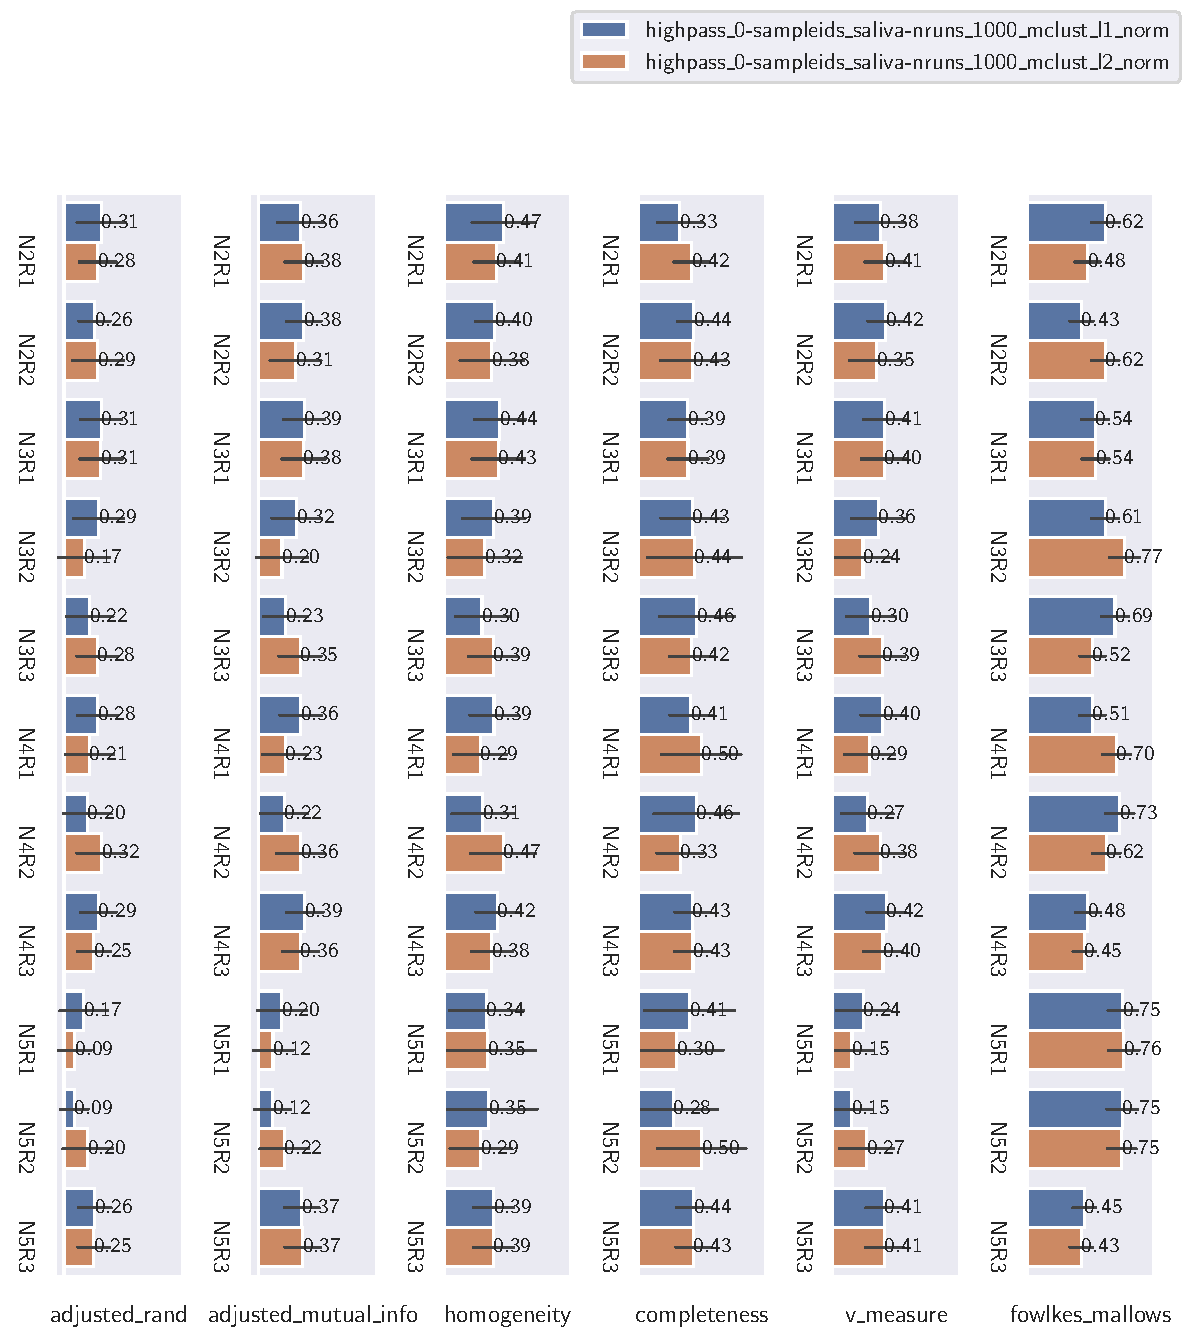
\includegraphics[width=\textwidth]{./figures/clust_comparison/highpass_0-sampleids_saliva-nruns_1000_mclust.pdf}
\caption{Mclust clustering performance metrics using 1000 trials sampled from EPGs from only saliva samples without high-pass filtering}
\label{fig:highpass_0-sampleids_saliva-nruns_1000_mclust}
\end{figure}

\begin{table}[H]
\centering
\maxsizebox{\textwidth}{0.65\textwidth}{
\begin{tabular}{llrrrr}
\toprule
     & {} & \multicolumn{2}{l}{homogeneity} & \multicolumn{2}{l}{completeness} \\
     & clusterer &           1 &      2 &            1 &      2 \\
\midrule
N2R1 & ci\_upp &       0.73\% &  0.38\% &        1.83\% &  0.38\% \\
     & success &       0.20\% &  0.00\% &        1.00\% &  0.00\% \\
     & ci\_low &       0.05\% &  0.00\% &        0.54\% &  0.00\% \\
N2R2 & ci\_upp &       0.38\% &  0.38\% &        0.38\% & 11.91\% \\
     & success &       0.00\% &  0.00\% &        0.00\% &  9.90\% \\
     & ci\_low &       0.00\% &  0.00\% &        0.00\% &  8.20\% \\
N3R1 & ci\_upp &       0.38\% &  0.38\% &        0.38\% &  0.73\% \\
     & success &       0.00\% &  0.00\% &        0.00\% &  0.20\% \\
     & ci\_low &       0.00\% &  0.00\% &        0.00\% &  0.05\% \\
N3R2 & ci\_upp &       0.38\% &  5.86\% &       10.72\% & 29.53\% \\
     & success &       0.00\% &  4.40\% &        8.80\% & 26.70\% \\
     & ci\_low &       0.00\% &  3.29\% &        7.20\% & 24.05\% \\
N3R3 & ci\_upp &       0.38\% &  0.38\% &       18.82\% &  2.95\% \\
     & success &       0.00\% &  0.00\% &       16.40\% &  1.90\% \\
     & ci\_low &       0.00\% &  0.00\% &       14.23\% &  1.22\% \\
N4R1 & ci\_upp &       0.38\% &  0.38\% &        1.96\% & 23.22\% \\
     & success &       0.00\% &  0.00\% &        1.10\% & 20.60\% \\
     & ci\_low &       0.00\% &  0.00\% &        0.62\% & 18.21\% \\
N4R2 & ci\_upp &       1.44\% &  1.02\% &       24.88\% &  1.96\% \\
     & success &       0.70\% &  0.40\% &       22.20\% &  1.10\% \\
     & ci\_low &       0.34\% &  0.16\% &       19.73\% &  0.62\% \\
N4R3 & ci\_upp &       0.38\% &  0.38\% &        0.56\% &  1.30\% \\
     & success &       0.00\% &  0.00\% &        0.10\% &  0.60\% \\
     & ci\_low &       0.00\% &  0.00\% &        0.02\% &  0.28\% \\
N5R1 & ci\_upp &       6.42\% & 24.36\% &       25.19\% & 23.32\% \\
     & success &       4.90\% & 21.70\% &       22.50\% & 20.70\% \\
     & ci\_low &       3.73\% & 19.26\% &       20.02\% & 18.30\% \\
N5R2 & ci\_upp &      25.19\% &  1.70\% &       20.40\% & 29.94\% \\
     & success &      22.50\% &  0.90\% &       17.90\% & 27.10\% \\
     & ci\_low &      20.02\% &  0.47\% &       15.65\% & 24.44\% \\
N5R3 & ci\_upp &       0.38\% &  0.38\% &        1.02\% &  0.56\% \\
     & success &       0.00\% &  0.00\% &        0.40\% &  0.10\% \\
     & ci\_low &       0.00\% &  0.00\% &        0.16\% &  0.02\% \\
\bottomrule
\end{tabular}


}
\caption{Mclust clustering percentages of trials where no error occurs using 1000 trials sampled from EPGs from only saliva samples without high-pass filtering}
\label{table:highpass_0-sampleids_saliva-nruns_1000_mclust}
\end{table}

\subsection{Saliva Samples Only, with High-Pass Filtering}

\begin{figure}[H]
\centering
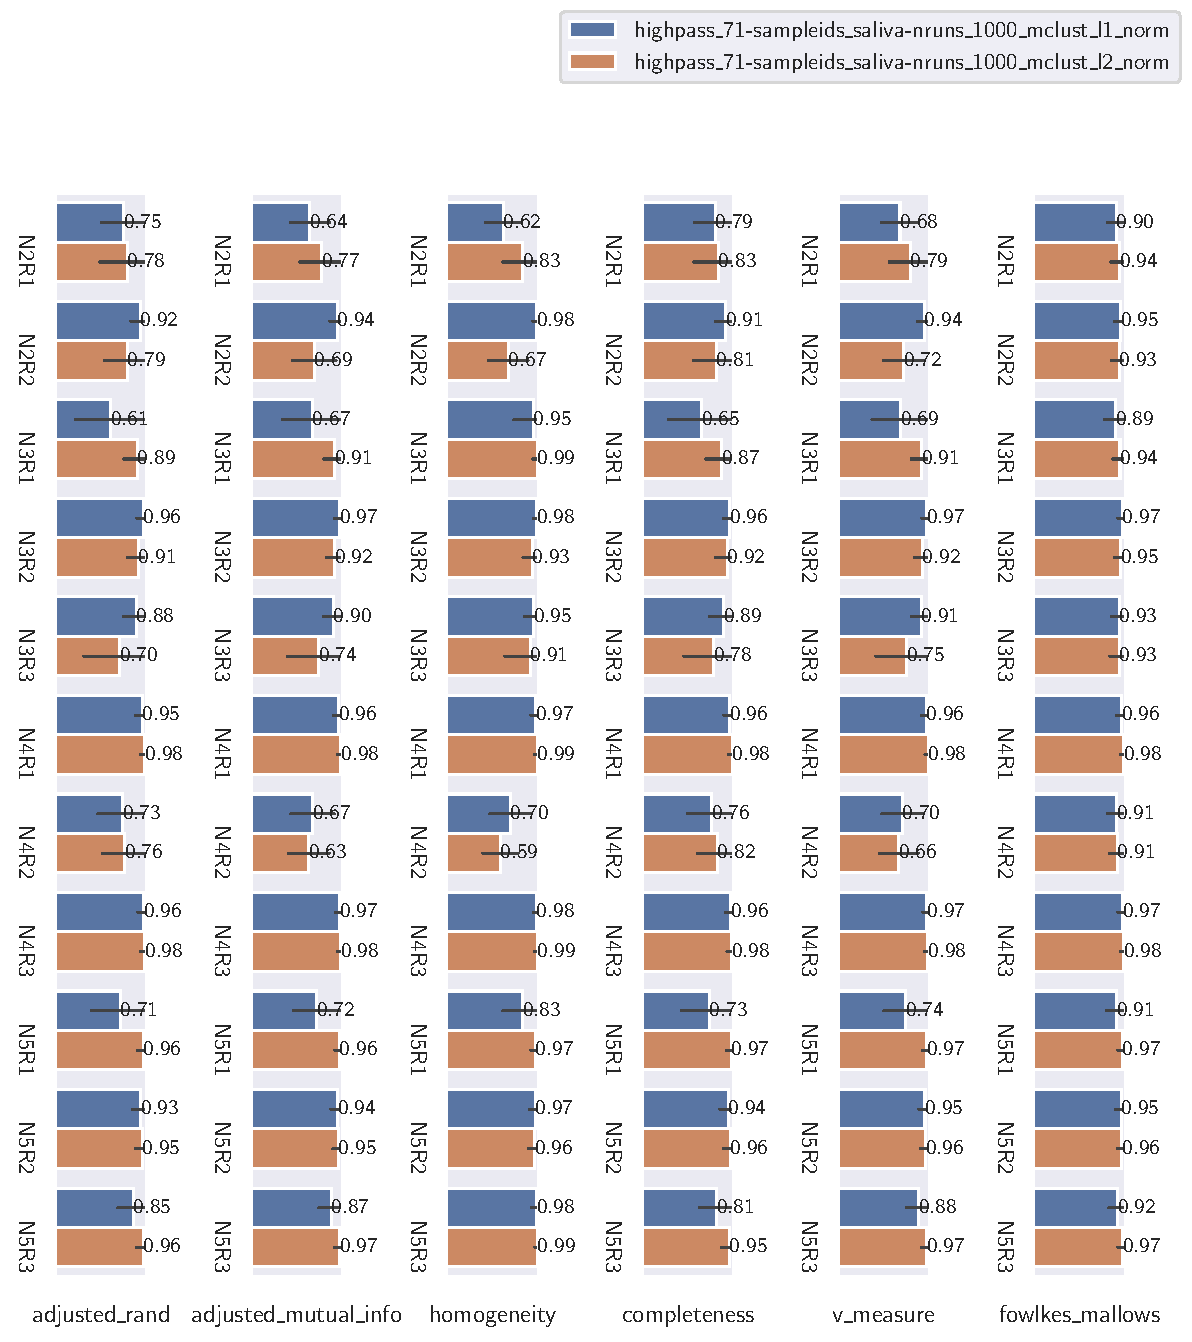
\includegraphics[width=\textwidth]{./figures/clust_comparison/highpass_71-sampleids_saliva-nruns_1000_mclust.pdf}
\caption{Mclust clustering performance metrics using 1000 trials sampled from EPGs from only saliva samples with high-pass filtering}
\label{fig:highpass_71-sampleids_saliva-nruns_1000_mclust}
\end{figure}

\begin{table}[H]
\centering
\maxsizebox{\textwidth}{0.65\textwidth}{
\begin{tabular}{llrrrr}
\toprule
     & {} & \multicolumn{2}{l}{homogeneity} & \multicolumn{2}{l}{completeness} \\
     & clusterer &           1 &      2 &            1 &      2 \\
\midrule
N2R1 & ci\_upp &       7.20\% & 43.88\% &       53.79\% & 72.57\% \\
     & success &       5.60\% & 40.80\% &       50.70\% & 69.80\% \\
     & ci\_low &       4.34\% & 37.79\% &       47.60\% & 66.88\% \\
N2R2 & ci\_upp &      82.27\% & 13.63\% &       59.34\% & 62.89\% \\
     & success &      79.90\% & 11.50\% &       56.30\% & 59.90\% \\
     & ci\_low &      77.30\% &  9.67\% &       53.21\% & 56.83\% \\
N3R1 & ci\_upp &      94.69\% & 94.15\% &       53.49\% & 64.17\% \\
     & success &      93.30\% & 92.70\% &       50.40\% & 61.20\% \\
     & ci\_low &      91.58\% & 90.92\% &       47.31\% & 58.14\% \\
N3R2 & ci\_upp &      73.82\% & 69.65\% &       65.25\% & 74.79\% \\
     & success &      71.10\% & 66.80\% &       62.30\% & 72.10\% \\
     & ci\_low &      68.21\% & 63.82\% &       59.25\% & 69.24\% \\
N3R3 & ci\_upp &      76.24\% & 92.07\% &       63.68\% & 71.69\% \\
     & success &      73.60\% & 90.40\% &       60.70\% & 68.90\% \\
     & ci\_low &      70.78\% & 88.42\% &       57.64\% & 65.96\% \\
N4R1 & ci\_upp &      62.99\% & 73.24\% &       59.15\% & 69.94\% \\
     & success &      60.00\% & 70.50\% &       56.10\% & 67.10\% \\
     & ci\_low &      56.93\% & 67.60\% &       53.01\% & 64.13\% \\
N4R2 & ci\_upp &      20.50\% &  3.19\% &       53.49\% & 58.36\% \\
     & success &      18.00\% &  2.10\% &       50.40\% & 55.30\% \\
     & ci\_low &      15.74\% &  1.38\% &       47.31\% & 52.20\% \\
N4R3 & ci\_upp &      64.37\% & 83.60\% &       59.94\% & 77.30\% \\
     & success &      61.40\% & 81.30\% &       56.90\% & 74.70\% \\
     & ci\_low &      58.34\% & 78.77\% &       53.81\% & 71.91\% \\
N5R1 & ci\_upp &      49.50\% & 64.37\% &       57.27\% & 66.52\% \\
     & success &      46.40\% & 61.40\% &       54.20\% & 63.60\% \\
     & ci\_low &      43.33\% & 58.34\% &       51.10\% & 60.57\% \\
N5R2 & ci\_upp &      70.33\% & 67.99\% &       61.42\% & 70.23\% \\
     & success &      67.50\% & 65.10\% &       58.40\% & 67.40\% \\
     & ci\_low &      64.53\% & 62.09\% &       55.32\% & 64.43\% \\
N5R3 & ci\_upp &      90.79\% & 90.05\% &       51.40\% & 73.44\% \\
     & success &      89.00\% & 88.20\% &       48.30\% & 70.70\% \\
     & ci\_low &      86.91\% & 86.05\% &       45.22\% & 67.80\% \\
\bottomrule
\end{tabular}


}
\caption{Mclust clustering percentages of trials where no error occurs using 1000 trials sampled from EPGs from only saliva samples with high-pass filtering}
\label{table:highpass_71-sampleids_saliva-nruns_1000_mclust}
\end{table}

\subsection{Blood Samples Only, without High-Pass Filtering}

\begin{figure}[H]
\centering
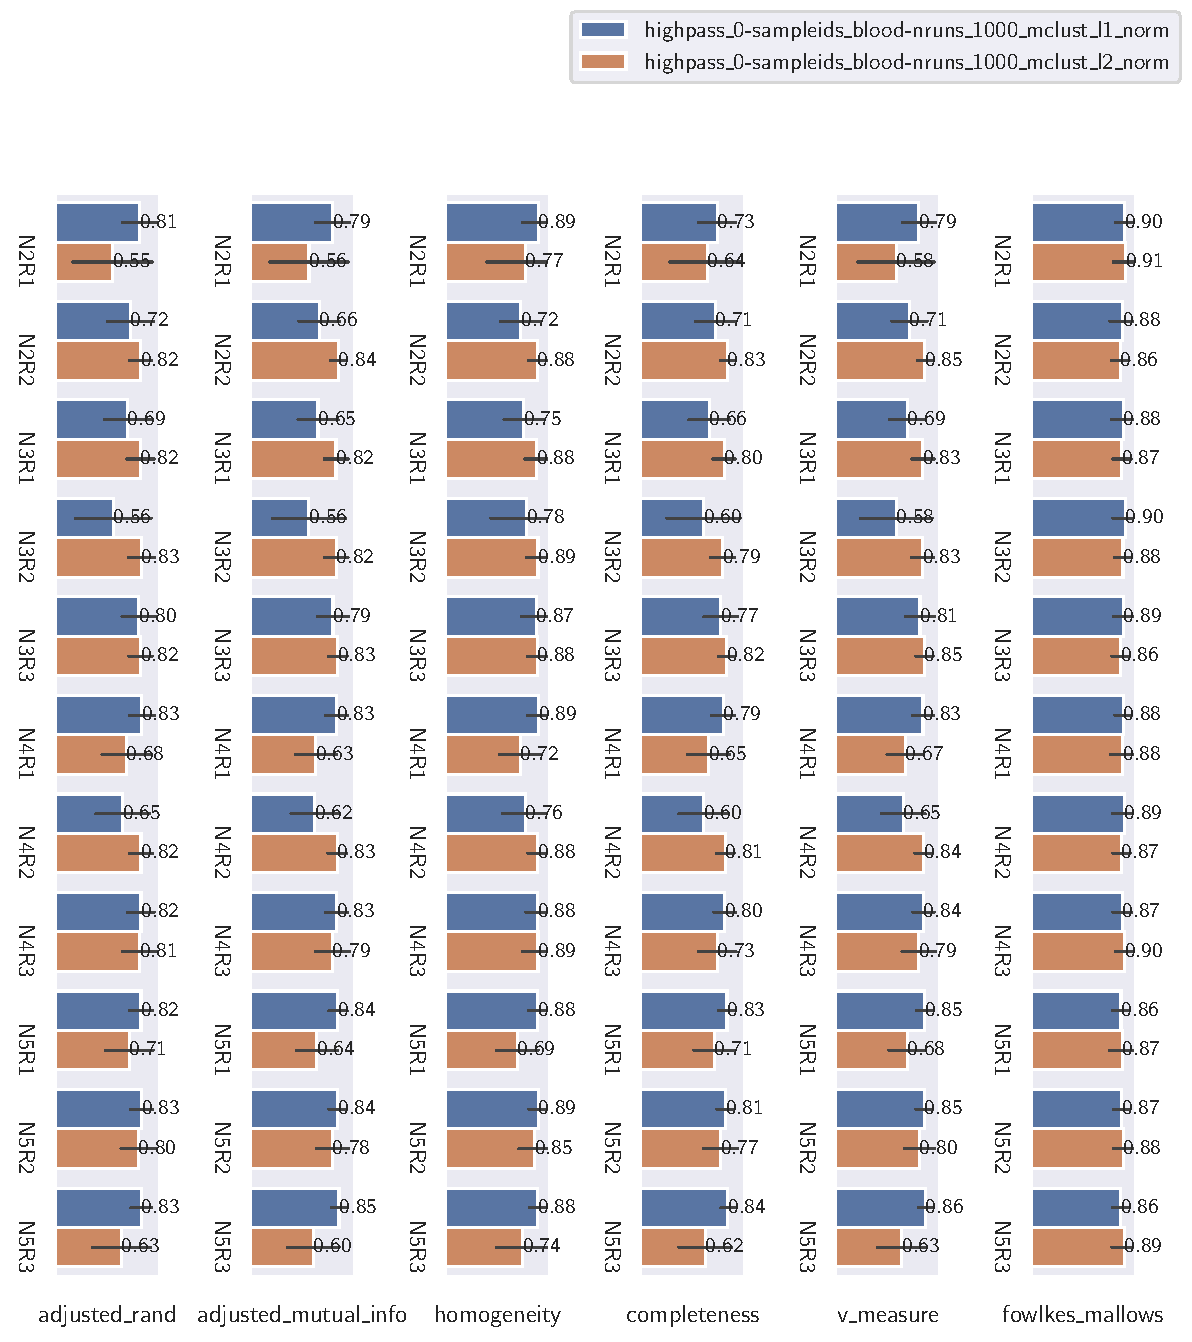
\includegraphics[width=\textwidth]{./figures/clust_comparison/highpass_0-sampleids_blood-nruns_1000_mclust.pdf}
\caption{Mclust clustering performance metrics using 1000 trials sampled from EPGs from only blood samples without high-pass filtering}
\label{fig:highpass_0-sampleids_blood-nruns_1000_mclust}
\end{figure}

\begin{table}[H]
\centering
\maxsizebox{\textwidth}{0.65\textwidth}{
\begin{tabular}{llrrrr}
\toprule
     & {} & \multicolumn{2}{l}{homogeneity} & \multicolumn{2}{l}{completeness} \\
     & clusterer &           1 &      2 &            1 &      2 \\
\midrule
N2R1 & ci\_upp &      40.95\% & 69.84\% &       21.44\% & 50.30\% \\
     & success &      37.90\% & 67.00\% &       18.90\% & 47.20\% \\
     & ci\_low &      34.94\% & 64.03\% &       16.59\% & 44.12\% \\
N2R2 & ci\_upp &      16.61\% &  1.02\% &       16.08\% &  0.73\% \\
     & success &      14.30\% &  0.40\% &       13.80\% &  0.20\% \\
     & ci\_low &      12.27\% &  0.16\% &       11.80\% &  0.05\% \\
N3R1 & ci\_upp &      23.53\% &  8.64\% &       13.41\% &  4.83\% \\
     & success &      20.90\% &  6.90\% &       11.30\% &  3.50\% \\
     & ci\_low &      18.49\% &  5.49\% &        9.48\% &  2.53\% \\
N3R2 & ci\_upp &      67.01\% & 10.61\% &       44.38\% &  6.64\% \\
     & success &      64.10\% &  8.70\% &       41.30\% &  5.10\% \\
     & ci\_low &      61.08\% &  7.11\% &       38.29\% &  3.90\% \\
N3R3 & ci\_upp &      29.84\% &  2.95\% &       20.08\% &  1.83\% \\
     & success &      27.00\% &  1.90\% &       17.60\% &  1.00\% \\
     & ci\_low &      24.34\% &  1.22\% &       15.36\% &  0.54\% \\
N4R1 & ci\_upp &      11.26\% & 20.19\% &        6.19\% & 12.45\% \\
     & success &       9.30\% & 17.70\% &        4.70\% & 10.40\% \\
     & ci\_low &       7.65\% & 15.46\% &        3.55\% &  8.66\% \\
N4R2 & ci\_upp &      35.67\% &  3.78\% &       19.56\% &  2.46\% \\
     & success &      32.70\% &  2.60\% &       17.10\% &  1.50\% \\
     & ci\_low &      29.86\% &  1.78\% &       14.89\% &  0.91\% \\
N4R3 & ci\_upp &       9.19\% & 41.35\% &        4.83\% & 22.49\% \\
     & success &       7.40\% & 38.30\% &        3.50\% & 19.90\% \\
     & ci\_low &       5.94\% & 35.34\% &        2.53\% & 17.54\% \\
N5R1 & ci\_upp &       3.31\% & 13.95\% &        1.83\% & 16.82\% \\
     & success &       2.20\% & 11.80\% &        1.00\% & 14.50\% \\
     & ci\_low &       1.46\% &  9.95\% &        0.54\% & 12.45\% \\
N5R2 & ci\_upp &       3.66\% & 29.12\% &        1.83\% & 20.92\% \\
     & success &       2.50\% & 26.30\% &        1.00\% & 18.40\% \\
     & ci\_low &       1.70\% & 23.67\% &        0.54\% & 16.12\% \\
N5R3 & ci\_upp &       1.30\% & 35.57\% &        0.73\% & 22.49\% \\
     & success &       0.60\% & 32.60\% &        0.20\% & 19.90\% \\
     & ci\_low &       0.28\% & 29.77\% &        0.05\% & 17.54\% \\
\bottomrule
\end{tabular}


}
\caption{Mclust clustering percentages of trials where no error occurs using 1000 trials sampled from EPGs from only blood samples without high-pass filtering}
\label{table:highpass_0-sampleids_blood-nruns_1000_mclust}
\end{table}

\subsection{Blood Samples Only, with High-Pass Filtering}

\begin{figure}[H]
\centering
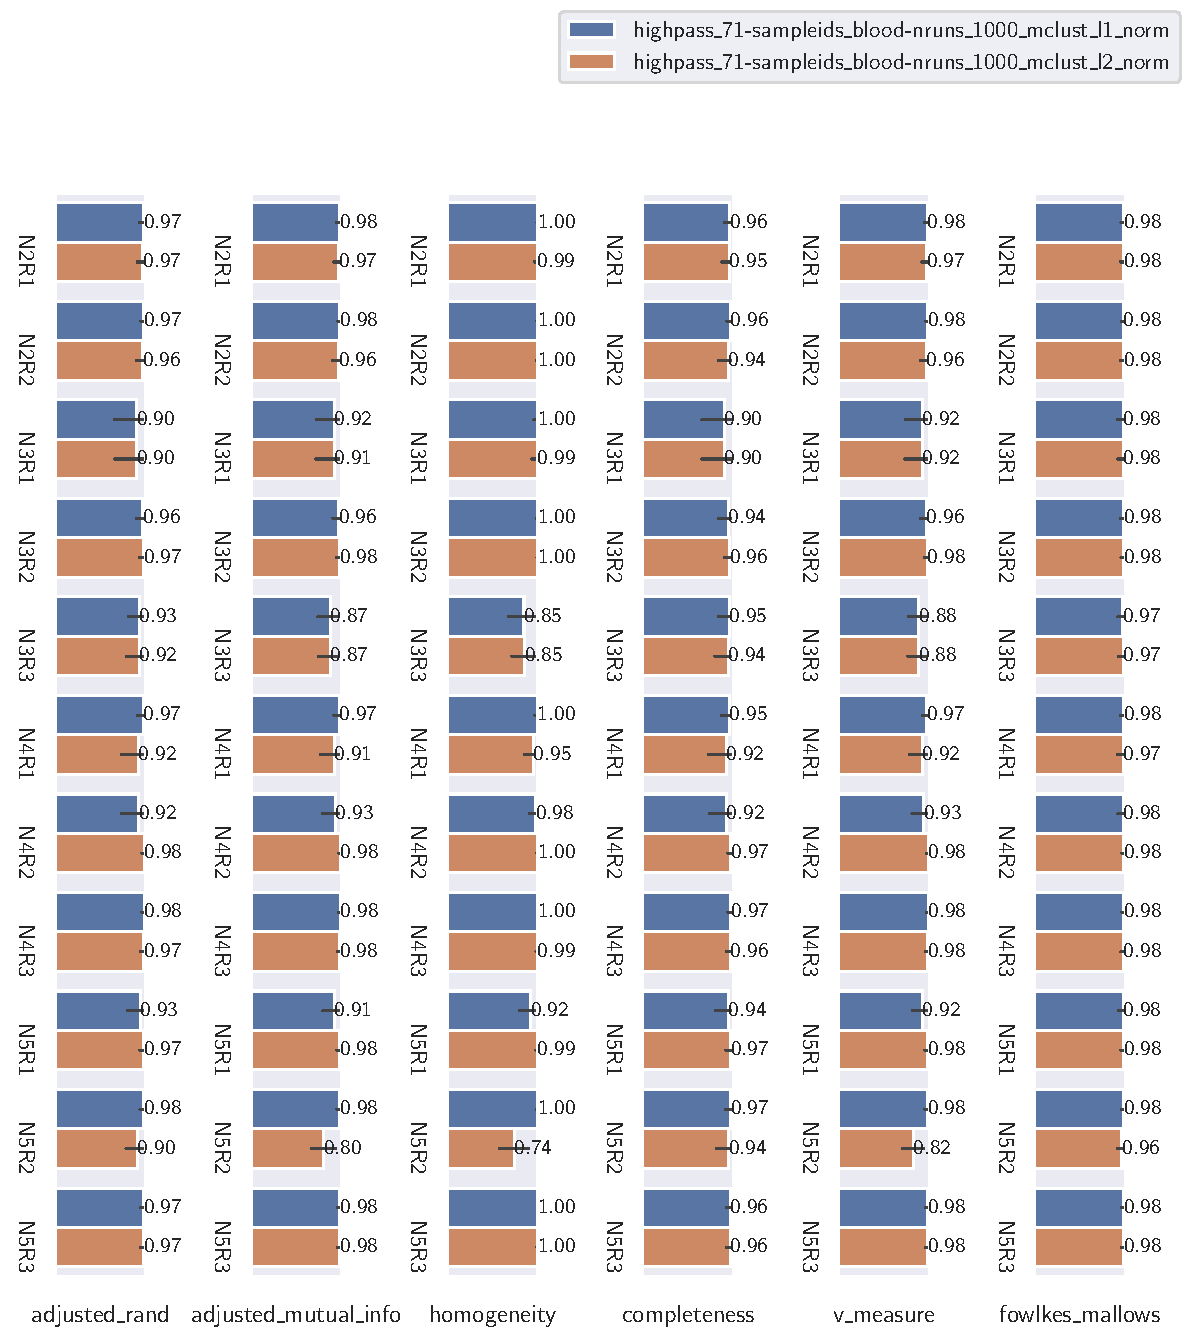
\includegraphics[width=\textwidth]{./figures/clust_comparison/highpass_71-sampleids_blood-nruns_1000_mclust.pdf}
\caption{Mclust clustering performance metrics using 1000 trials sampled from EPGs from only blood samples with high-pass filtering}
\label{fig:highpass_71-sampleids_blood-nruns_1000_mclust}
\end{figure}

\begin{table}[H]
\centering
\maxsizebox{\textwidth}{0.65\textwidth}{
\begin{tabular}{llrrrr}
\toprule
     & {} & \multicolumn{2}{l}{homogeneity} & \multicolumn{2}{l}{completeness} \\
     & clusterer &           1 &      2 &            1 &      2 \\
\midrule
N2R1 & ci\_upp &      98.62\% & 94.69\% &       70.33\% & 78.74\% \\
     & success &      97.90\% & 93.30\% &       67.50\% & 76.20\% \\
     & ci\_low &      96.81\% & 91.58\% &       64.53\% & 73.46\% \\
N2R2 & ci\_upp &      92.17\% & 99.24\% &       55.58\% & 78.45\% \\
     & success &      90.50\% & 98.70\% &       52.50\% & 75.90\% \\
     & ci\_low &      88.52\% & 97.79\% &       49.40\% & 73.15\% \\
N3R1 & ci\_upp &      99.90\% & 99.66\% &       86.61\% & 86.80\% \\
     & success &      99.70\% & 99.30\% &       84.50\% & 84.70\% \\
     & ci\_low &      99.12\% & 98.56\% &       82.13\% & 82.34\% \\
N3R2 & ci\_upp &      99.16\% & 98.62\% &       78.35\% & 70.62\% \\
     & success &      98.60\% & 97.90\% &       75.80\% & 67.80\% \\
     & ci\_low &      97.66\% & 96.81\% &       73.05\% & 64.84\% \\
N3R3 & ci\_upp &      54.49\% & 48.10\% &       86.61\% & 87.83\% \\
     & success &      51.40\% & 45.00\% &       84.50\% & 85.80\% \\
     & ci\_low &      48.30\% & 41.94\% &       82.13\% & 83.50\% \\
N4R1 & ci\_upp &      96.45\% & 77.68\% &       78.45\% & 86.42\% \\
     & success &      95.30\% & 75.10\% &       75.90\% & 84.30\% \\
     & ci\_low &      93.81\% & 72.33\% &       73.15\% & 81.91\% \\
N4R2 & ci\_upp &      89.13\% & 95.05\% &       86.42\% & 53.39\% \\
     & success &      87.20\% & 93.70\% &       84.30\% & 50.30\% \\
     & ci\_low &      84.99\% & 92.02\% &       81.91\% & 47.21\% \\
N4R3 & ci\_upp &      96.88\% & 87.73\% &       53.29\% & 55.48\% \\
     & success &      95.80\% & 85.70\% &       50.20\% & 52.40\% \\
     & ci\_low &      94.37\% & 83.39\% &       47.11\% & 49.30\% \\
N5R1 & ci\_upp &      71.89\% & 92.35\% &       87.64\% & 71.60\% \\
     & success &      69.10\% & 90.70\% &       85.60\% & 68.80\% \\
     & ci\_low &      66.17\% & 88.74\% &       83.29\% & 65.86\% \\
N5R2 & ci\_upp &      95.66\% & 25.71\% &       71.89\% & 86.80\% \\
     & success &      94.40\% & 23.00\% &       69.10\% & 84.70\% \\
     & ci\_low &      92.80\% & 20.50\% &       66.17\% & 82.34\% \\
N5R3 & ci\_upp &      97.30\% & 96.19\% &       59.05\% & 59.05\% \\
     & success &      96.30\% & 95.00\% &       56.00\% & 56.00\% \\
     & ci\_low &      94.94\% & 93.47\% &       52.91\% & 52.91\% \\
\bottomrule
\end{tabular}


}
\caption{Mclust clustering percentages of trials where no error occurs using 1000 trials sampled from EPGs from only blood samples with high-pass filtering}
\label{table:highpass_71-sampleids_blood-nruns_1000_mclust}
\end{table}

\subsection{All Samples, without High-Pass Filtering}

\begin{figure}[H]
\centering
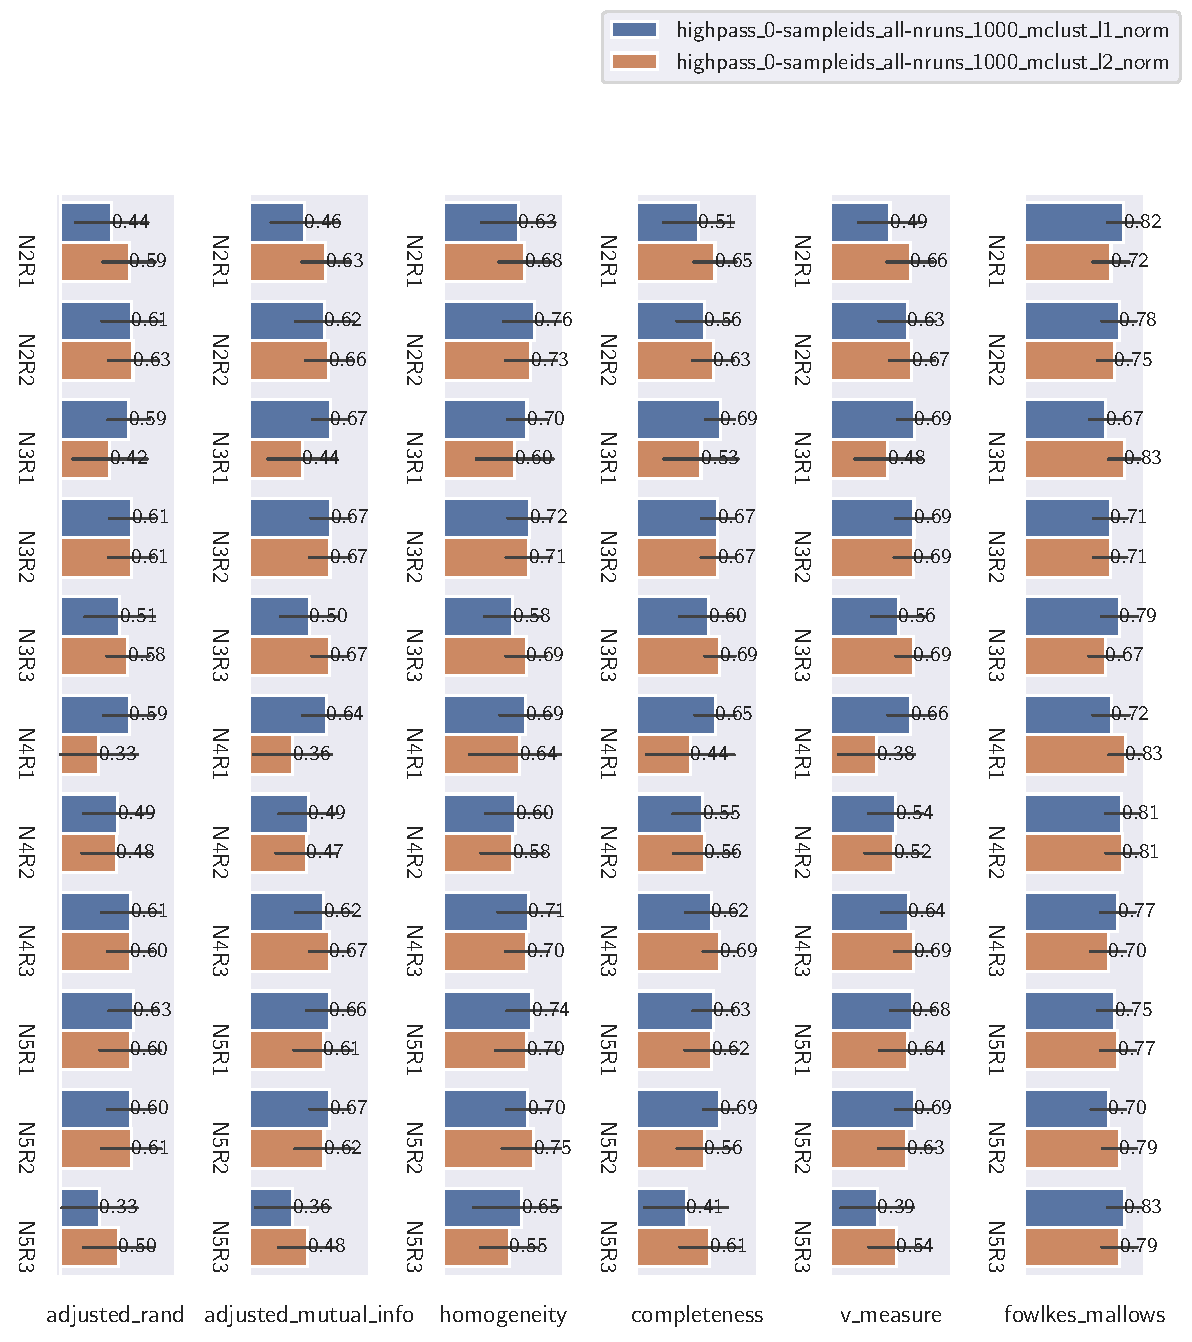
\includegraphics[width=\textwidth]{./figures/clust_comparison/highpass_0-sampleids_all-nruns_1000_mclust.pdf}
\caption{Mclust clustering performance metrics using 1000 trials sampled from all EPGs without high-pass filtering}
\label{fig:highpass_0-sampleids_all-nruns_1000_mclust}
\end{figure}

\begin{table}[H]
\centering
\maxsizebox{\textwidth}{0.65\textwidth}{
\begin{tabular}{llrrrr}
\toprule
     & {} & \multicolumn{2}{l}{homogeneity} & \multicolumn{2}{l}{completeness} \\
     & clusterer &           1 &      2 &            1 &      2 \\
\midrule
N2R1 & ci\_upp &      23.63\% &  2.46\% &       19.66\% &  1.57\% \\
     & success &      21.00\% &  1.50\% &       17.20\% &  0.80\% \\
     & ci\_low &      18.59\% &  0.91\% &       14.99\% &  0.41\% \\
N2R2 & ci\_upp &      27.57\% &  4.48\% &        9.30\% &  1.57\% \\
     & success &      24.80\% &  3.20\% &        7.50\% &  0.80\% \\
     & ci\_low &      22.22\% &  2.28\% &        6.03\% &  0.41\% \\
N3R1 & ci\_upp &       0.38\% & 22.70\% &        0.38\% & 23.94\% \\
     & success &       0.00\% & 20.10\% &        0.00\% & 21.30\% \\
     & ci\_low &       0.00\% & 17.73\% &        0.00\% & 18.87\% \\
N3R2 & ci\_upp &       0.88\% &  0.73\% &        0.73\% &  0.73\% \\
     & success &       0.30\% &  0.20\% &        0.20\% &  0.20\% \\
     & ci\_low &       0.10\% &  0.05\% &        0.05\% &  0.05\% \\
N3R3 & ci\_upp &       5.17\% &  0.38\% &       14.27\% &  0.38\% \\
     & success &       3.80\% &  0.00\% &       12.10\% &  0.00\% \\
     & ci\_low &       2.78\% &  0.00\% &       10.22\% &  0.00\% \\
N4R1 & ci\_upp &       2.58\% & 53.59\% &        1.70\% & 29.73\% \\
     & success &       1.60\% & 50.50\% &        0.90\% & 26.90\% \\
     & ci\_low &       0.99\% & 47.41\% &        0.47\% & 24.24\% \\
N4R2 & ci\_upp &       9.08\% &  8.75\% &       11.04\% & 14.59\% \\
     & success &       7.30\% &  7.00\% &        9.10\% & 12.40\% \\
     & ci\_low &       5.85\% &  5.58\% &        7.47\% & 10.50\% \\
N4R3 & ci\_upp &      14.59\% &  0.73\% &        8.64\% &  0.88\% \\
     & success &      12.40\% &  0.20\% &        6.90\% &  0.30\% \\
     & ci\_low &      10.50\% &  0.05\% &        5.49\% &  0.10\% \\
N5R1 & ci\_upp &       5.06\% & 14.59\% &        1.96\% & 10.28\% \\
     & success &       3.70\% & 12.40\% &        1.10\% &  8.40\% \\
     & ci\_low &       2.70\% & 10.50\% &        0.62\% &  6.84\% \\
N5R2 & ci\_upp &       0.56\% & 27.36\% &        0.73\% &  9.63\% \\
     & success &       0.10\% & 24.60\% &        0.20\% &  7.80\% \\
     & ci\_low &       0.02\% & 22.03\% &        0.05\% &  6.29\% \\
N5R3 & ci\_upp &      52.69\% &  4.25\% &       24.78\% & 16.08\% \\
     & success &      49.60\% &  3.00\% &       22.10\% & 13.80\% \\
     & ci\_low &      46.51\% &  2.11\% &       19.64\% & 11.80\% \\
\bottomrule
\end{tabular}


}
\caption{Mclust clustering percentages of trials where no error occurs using 1000 trials sampled from all EPGs without high-pass filtering}
\label{table:highpass_0-sampleids_all-nruns_1000_mclust}
\end{table}

\subsection{All Samples, with High-Pass Filtering}

\begin{figure}[H]
\centering
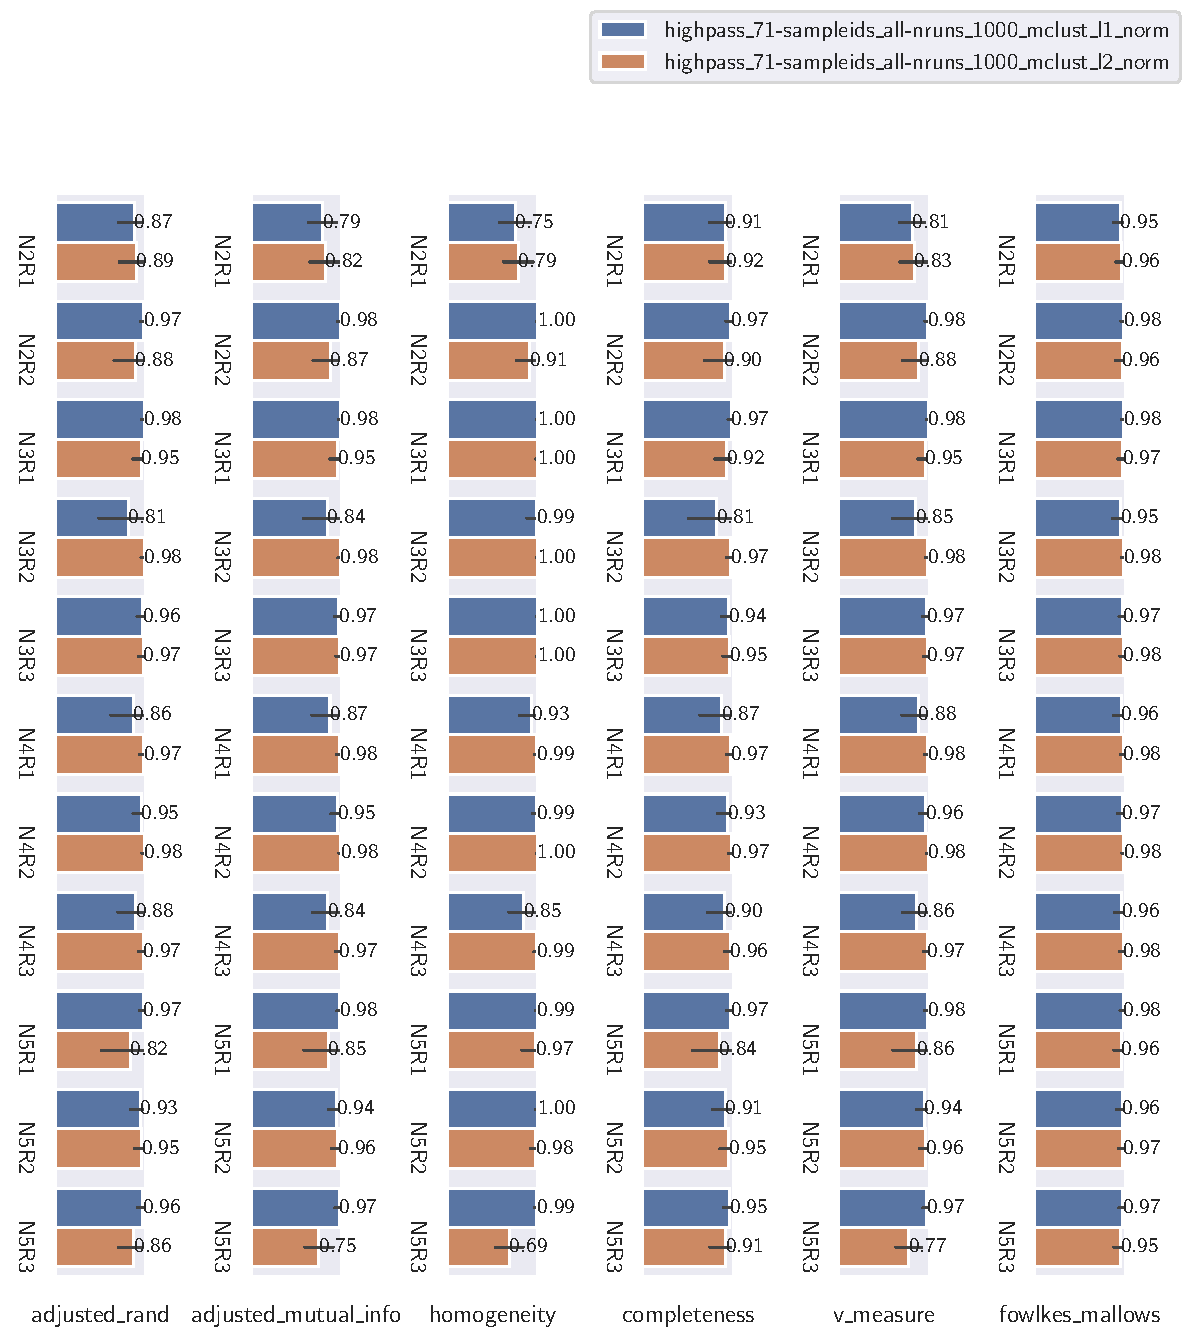
\includegraphics[width=\textwidth]{./figures/clust_comparison/highpass_71-sampleids_all-nruns_1000_mclust.pdf}
\caption{Mclust clustering performance metrics using 1000 trials sampled from all EPGs with high-pass filtering}
\label{fig:highpass_71-sampleids_all-nruns_1000_mclust}
\end{figure}

\begin{table}[H]
\centering
\maxsizebox{\textwidth}{0.65\textwidth}{
\begin{tabular}{llrrrr}
\toprule
     & {} & \multicolumn{2}{l}{homogeneity} & \multicolumn{2}{l}{completeness} \\
     & clusterer &           1 &      2 &            1 &      2 \\
\midrule
N2R1 & ci\_upp &      23.94\% & 27.16\% &       77.87\% & 83.97\% \\
     & success &      21.30\% & 24.40\% &       75.30\% & 81.70\% \\
     & ci\_low &      18.87\% & 21.84\% &       72.53\% & 79.18\% \\
N2R2 & ci\_upp &      94.06\% & 64.27\% &       65.06\% & 83.31\% \\
     & success &      92.60\% & 61.30\% &       62.10\% & 81.00\% \\
     & ci\_low &      90.81\% & 58.24\% &       59.05\% & 78.45\% \\
N3R1 & ci\_upp &      90.88\% & 99.01\% &       59.05\% & 76.24\% \\
     & success &      89.10\% & 98.40\% &       56.00\% & 73.60\% \\
     & ci\_low &      87.02\% & 97.42\% &       52.91\% & 70.78\% \\
N3R2 & ci\_upp &      98.94\% & 94.87\% &       75.85\% & 68.09\% \\
     & success &      98.30\% & 93.50\% &       73.20\% & 65.20\% \\
     & ci\_low &      97.29\% & 91.80\% &       70.37\% & 62.19\% \\
N3R3 & ci\_upp &      96.71\% & 97.05\% &       66.33\% & 71.21\% \\
     & success &      95.60\% & 96.00\% &       63.40\% & 68.40\% \\
     & ci\_low &      94.14\% & 94.60\% &       60.37\% & 65.45\% \\
N4R1 & ci\_upp &      74.60\% & 82.74\% &       78.54\% & 62.11\% \\
     & success &      71.90\% & 80.40\% &       76.00\% & 59.10\% \\
     & ci\_low &      69.03\% & 77.83\% &       73.26\% & 56.02\% \\
N4R2 & ci\_upp &      93.53\% & 89.31\% &       74.89\% & 60.63\% \\
     & success &      92.00\% & 87.40\% &       72.20\% & 57.60\% \\
     & ci\_low &      90.15\% & 85.20\% &       69.34\% & 54.51\% \\
N4R3 & ci\_upp &      45.49\% & 87.17\% &       80.65\% & 69.94\% \\
     & success &      42.40\% & 85.10\% &       78.20\% & 67.10\% \\
     & ci\_low &      39.37\% & 82.76\% &       75.54\% & 64.13\% \\
N5R1 & ci\_upp &      85.39\% & 97.89\% &       61.12\% & 79.69\% \\
     & success &      83.20\% & 97.00\% &       58.10\% & 77.20\% \\
     & ci\_low &      80.76\% & 95.75\% &       55.02\% & 74.50\% \\
N5R2 & ci\_upp &      98.62\% & 89.31\% &       71.89\% & 79.41\% \\
     & success &      97.90\% & 87.40\% &       69.10\% & 76.90\% \\
     & ci\_low &      96.81\% & 85.20\% &       66.17\% & 74.19\% \\
N5R3 & ci\_upp &      88.94\% & 11.04\% &       65.84\% & 79.69\% \\
     & success &      87.00\% &  9.10\% &       62.90\% & 77.20\% \\
     & ci\_low &      84.77\% &  7.47\% &       59.86\% & 74.50\% \\
\bottomrule
\end{tabular}


}
\caption{Mclust clustering percentages of trials where no error occurs using 1000 trials sampled from all EPGs with high-pass filtering}
\label{table:highpass_71-sampleids_all-nruns_1000_mclust}
\end{table}

%--------------------------------------------------------------------------------------------------------------------------------------------
\section{Experiments Results---Individual Clusterers}

\subsection{Saliva Samples Only, without High-Pass Filtering}

\begin{table}[H]
\centering
\maxsizebox{\textwidth}{0.65\textwidth}{
\begin{tabular}{lrr}
\toprule
{} &      mean &       std \\
clusterer                                          &           &           \\
\midrule
affinity\_l2\_norm                                   &  0.537845 &  0.193364 \\
hdbscan\_cosine\_epsilon\_0.0\_eom\_per\_locus\_norm      &  0.494584 &  0.274283 \\
hdbscan\_cosine\_epsilon\_0.0\_eom\_per\_locus\_quantize  &  0.486221 &  0.265297 \\
hdbscan\_cosine\_epsilon\_0.5\_leaf\_per\_locus\_norm     &  0.484973 &  0.267075 \\
hdbscan\_cosine\_epsilon\_0.5\_eom\_per\_locus\_norm      &  0.484847 &  0.271220 \\
affinity\_l1\_norm                                   &  0.473349 &  0.236314 \\
hdbscan\_euclidean\_epsilon\_0.5\_eom\_l2\_norm          &  0.464676 &  0.261550 \\
hdbscan\_euclidean\_epsilon\_0.0\_eom\_l2\_norm          &  0.464474 &  0.261570 \\
birch\_per\_locus\_norm                               &  0.461531 &  0.176776 \\
birch\_per\_locus\_quantize                           &  0.461388 &  0.176951 \\
hdbscan\_cosine\_epsilon\_0.0\_eom                     &  0.457188 &  0.258795 \\
birch\_l2\_norm                                      &  0.450668 &  0.201137 \\
hdbscan\_cosine\_epsilon\_0.0\_leaf\_per\_locus\_norm     &  0.447478 &  0.262407 \\
hdbscan\_euclidean\_epsilon\_0.5\_leaf\_l2\_norm         &  0.444169 &  0.259896 \\
affinity\_per\_locus\_quantize                        &  0.438395 &  0.174343 \\
meanshift\_per\_locus\_norm                           &  0.431335 &  0.263610 \\
affinity\_per\_locus\_norm                            &  0.429782 &  0.173224 \\
meanshift\_per\_locus\_quantize                       &  0.429451 &  0.259660 \\
hdbscan\_cosine\_epsilon\_0.0\_leaf\_per\_locus\_quantize &  0.429403 &  0.250309 \\
hdbscan\_euclidean\_epsilon\_0.0\_leaf\_l2\_norm         &  0.428211 &  0.254899 \\
optics\_l2\_norm                                     &  0.414122 &  0.255132 \\
hdbscan\_cosine\_epsilon\_0.0\_leaf                    &  0.409896 &  0.247945 \\
hdbscan\_euclidean\_epsilon\_1.0\_leaf\_l2\_norm         &  0.401358 &  0.250626 \\
hdbscan\_euclidean\_epsilon\_1.0\_eom\_l2\_norm          &  0.400522 &  0.251545 \\
hdbscan\_cosine\_epsilon\_0.5\_leaf                    &  0.394007 &  0.250049 \\
\bottomrule
\end{tabular}


}
\caption{Top 25 clusterers by arithmetic mean of clustering metric scores, using admixtures sampled from only saliva EPG data without highpass filter}
\label{table:top_25_not_ensemble_clusterers_by_metrics_highpass_0-sampleids_saliva-nruns_1000}
\end{table}

\begin{figure}[H]
\centering
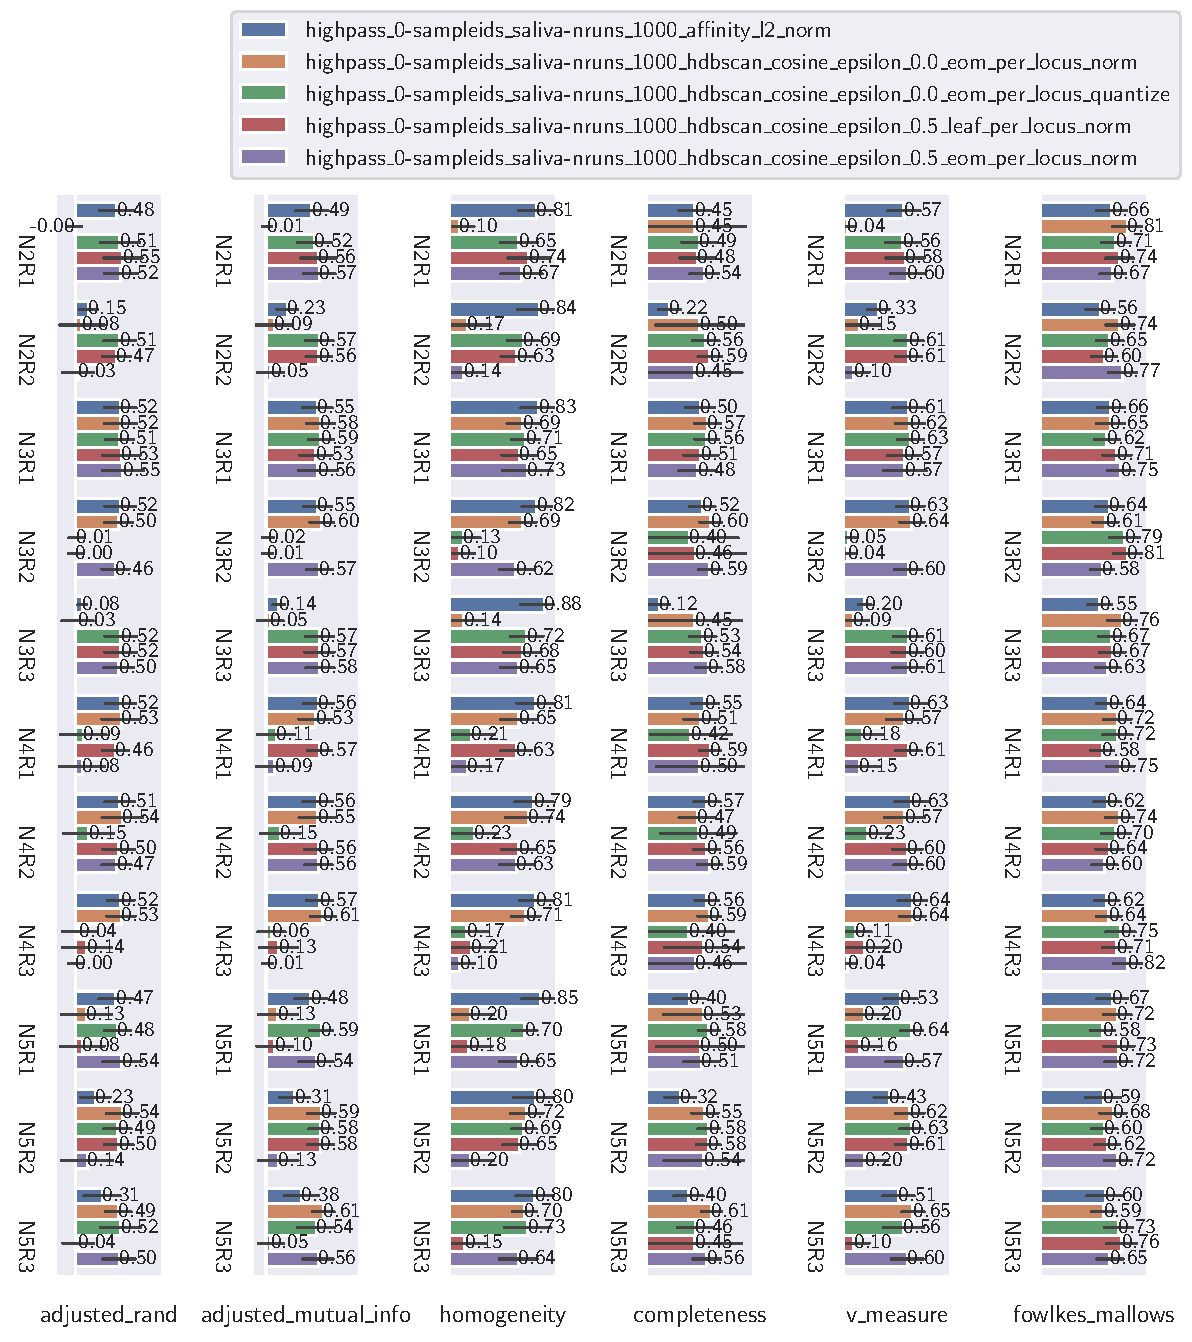
\includegraphics[width=\textwidth]{./figures/clust_comparison/highpass_0-sampleids_saliva-nruns_1000_top_5_clusterers_by_metrics.pdf}
\caption{Top 5 clusterers clustering performance metrics using 1000 trials sampled from EPGs from only saliva samples without high-pass filtering}
\label{fig:highpass_0-sampleids_saliva-nruns_1000_top_5_clusterers_by_metrics}
\end{figure}

\begin{table}[H]
\centering
\maxsizebox{\textwidth}{0.65\textwidth}{
\begin{tabular}{lrr}
\toprule
{} &  mean &   std \\
clusterer                                         &       &       \\
\midrule
meanshift\_per\_locus\_norm                          & 1.13\% & 2.13\% \\
meanshift\_per\_locus\_quantize                      & 1.03\% & 2.05\% \\
birch\_l2\_norm                                     & 0.21\% & 0.27\% \\
hdbscan\_cosine\_epsilon\_1.0\_eom\_per\_locus\_norm     & 0.18\% & 0.25\% \\
hdbscan\_cosine\_epsilon\_1.0\_leaf\_per\_locus\_norm    & 0.18\% & 0.25\% \\
mclust\_l2\_norm                                    & 0.18\% & 0.28\% \\
hdbscan\_cosine\_epsilon\_0.0\_eom\_per\_locus\_norm     & 0.17\% & 0.24\% \\
hdbscan\_cosine\_epsilon\_0.5\_eom\_per\_locus\_norm     & 0.17\% & 0.24\% \\
hdbscan\_cosine\_epsilon\_0.5\_leaf\_per\_locus\_norm    & 0.17\% & 0.24\% \\
optics\_l2\_norm                                    & 0.16\% & 0.22\% \\
hdbscan\_cosine\_epsilon\_0.5\_eom                    & 0.16\% & 0.24\% \\
hdbscan\_cosine\_epsilon\_0.5\_leaf                   & 0.16\% & 0.24\% \\
hdbscan\_cosine\_epsilon\_1.0\_eom                    & 0.16\% & 0.24\% \\
hdbscan\_cosine\_epsilon\_1.0\_leaf                   & 0.16\% & 0.24\% \\
hdbscan\_euclidean\_epsilon\_1.0\_eom\_l2\_norm         & 0.16\% & 0.24\% \\
hdbscan\_euclidean\_epsilon\_1.0\_leaf\_l2\_norm        & 0.16\% & 0.24\% \\
hdbscan\_cosine\_epsilon\_0.0\_eom\_per\_locus\_quantize & 0.15\% & 0.21\% \\
hdbscan\_cosine\_epsilon\_0.0\_leaf\_per\_locus\_norm    & 0.15\% & 0.21\% \\
hdbscan\_cosine\_epsilon\_0.0\_eom                    & 0.15\% & 0.22\% \\
hdbscan\_euclidean\_epsilon\_0.0\_eom\_l2\_norm         & 0.15\% & 0.22\% \\
hdbscan\_euclidean\_epsilon\_0.5\_eom\_l2\_norm         & 0.15\% & 0.22\% \\
optics\_per\_locus\_norm                             & 0.15\% & 0.22\% \\
optics\_per\_locus\_quantize                         & 0.15\% & 0.22\% \\
hdbscan\_cosine\_epsilon\_0.0\_leaf                   & 0.15\% & 0.20\% \\
hdbscan\_euclidean\_epsilon\_0.0\_leaf\_l2\_norm        & 0.15\% & 0.20\% \\
\bottomrule
\end{tabular}


}
\caption{Top 25 clusterers by arithmetic mean of percentages of perfect clustering, using admixtures sampled from only saliva EPG data without highpass filter}
\label{table:top_25_not_ensemble_clusterers_by_binomial_confidence_highpass_0-sampleids_saliva-nruns_1000}
\end{table}

\begin{table}[H]
\centering
\maxsizebox{\textwidth}{0.65\textwidth}{
\begin{tabular}{llrrrrrrrrrr}
\toprule
     & {} & \multicolumn{5}{l}{homogeneity} & \multicolumn{5}{l}{completeness} \\
     & clusterer &           1 &      2 &      3 &      4 &      5 &            1 &      2 &     3 &      4 &      5 \\
\midrule
N2R1 & ci\_upp &       0.38\% &  3.19\% &  0.38\% &  0.38\% &  0.38\% &       42.67\% & 14.16\% & 0.73\% & 39.43\% &  0.38\% \\
     & success &       0.00\% &  2.10\% &  0.00\% &  0.00\% &  0.00\% &       39.60\% & 12.00\% & 0.20\% & 36.40\% &  0.00\% \\
     & ci\_low &       0.00\% &  1.38\% &  0.00\% &  0.00\% &  0.00\% &       36.61\% & 10.13\% & 0.05\% & 33.48\% &  0.00\% \\
N2R2 & ci\_upp &       0.38\% &  0.38\% &  0.38\% &  0.38\% & 10.83\% &       56.18\% & 32.61\% & 1.30\% &  0.38\% &  0.88\% \\
     & success &       0.00\% &  0.00\% &  0.00\% &  0.00\% &  8.90\% &       53.10\% & 29.70\% & 0.60\% &  0.00\% &  0.30\% \\
     & ci\_low &       0.00\% &  0.00\% &  0.00\% &  0.00\% &  7.29\% &       50.00\% & 26.95\% & 0.28\% &  0.00\% &  0.10\% \\
N3R1 & ci\_upp &       0.38\% & 22.07\% &  0.38\% &  0.56\% &  0.38\% &       35.16\% & 10.28\% & 0.38\% & 45.99\% & 40.85\% \\
     & success &       0.00\% & 19.50\% &  0.00\% &  0.10\% &  0.00\% &       32.20\% &  8.40\% & 0.00\% & 42.90\% & 37.80\% \\
     & ci\_low &       0.00\% & 17.16\% &  0.00\% &  0.02\% &  0.00\% &       29.38\% &  6.84\% & 0.00\% & 39.87\% & 34.85\% \\
N3R2 & ci\_upp &       0.38\% &  0.38\% &  0.38\% &  1.02\% &  1.02\% &       54.88\% & 52.40\% & 0.38\% &  1.57\% &  1.57\% \\
     & success &       0.00\% &  0.00\% &  0.00\% &  0.40\% &  0.40\% &       51.80\% & 49.30\% & 0.00\% &  0.80\% &  0.80\% \\
     & ci\_low &       0.00\% &  0.00\% &  0.00\% &  0.16\% &  0.16\% &       48.70\% & 46.21\% & 0.00\% &  0.41\% &  0.41\% \\
N3R3 & ci\_upp &       6.98\% &  1.57\% &  1.02\% &  0.38\% &  0.38\% &        8.53\% & 12.66\% & 1.02\% &  0.38\% &  0.38\% \\
     & success &       5.40\% &  0.80\% &  0.40\% &  0.00\% &  0.00\% &        6.80\% & 10.60\% & 0.40\% &  0.00\% &  0.00\% \\
     & ci\_low &       4.16\% &  0.41\% &  0.16\% &  0.00\% &  0.00\% &        5.40\% &  8.84\% & 0.16\% &  0.00\% &  0.00\% \\
N4R1 & ci\_upp &       3.31\% &  0.38\% &  0.88\% &  0.38\% &  0.38\% &       19.24\% & 40.54\% & 0.88\% &  0.38\% &  0.38\% \\
     & success &       2.20\% &  0.00\% &  0.30\% &  0.00\% &  0.00\% &       16.80\% & 37.50\% & 0.30\% &  0.00\% &  0.00\% \\
     & ci\_low &       1.46\% &  0.00\% &  0.10\% &  0.00\% &  0.00\% &       14.61\% & 34.55\% & 0.10\% &  0.00\% &  0.00\% \\
N4R2 & ci\_upp &       1.02\% &  0.38\% &  0.38\% & 10.83\% &  0.56\% &       13.84\% & 43.17\% & 0.38\% &  0.88\% & 45.99\% \\
     & success &       0.40\% &  0.00\% &  0.00\% &  8.90\% &  0.10\% &       11.70\% & 40.10\% & 0.00\% &  0.30\% & 42.90\% \\
     & ci\_low &       0.16\% &  0.00\% &  0.00\% &  7.29\% &  0.02\% &        9.85\% & 37.11\% & 0.00\% &  0.10\% & 39.87\% \\
N4R3 & ci\_upp &       0.38\% &  5.40\% &  0.38\% &  0.38\% &  0.38\% &       43.88\% &  4.71\% & 0.38\% & 40.85\% & 36.18\% \\
     & success &       0.00\% &  4.00\% &  0.00\% &  0.00\% &  0.00\% &       40.80\% &  3.40\% & 0.00\% & 37.80\% & 33.20\% \\
     & ci\_low &       0.00\% &  2.95\% &  0.00\% &  0.00\% &  0.00\% &       37.79\% &  2.44\% & 0.00\% & 34.85\% & 30.35\% \\
N5R1 & ci\_upp &       2.09\% & 10.50\% &  9.30\% &  0.38\% &  0.38\% &        6.08\% &  7.20\% & 0.38\% & 36.18\% & 39.43\% \\
     & success &       1.20\% &  8.60\% &  7.50\% &  0.00\% &  0.00\% &        4.60\% &  5.60\% & 0.00\% & 33.20\% & 36.40\% \\
     & ci\_low &       0.69\% &  7.02\% &  6.03\% &  0.00\% &  0.00\% &        3.47\% &  4.34\% & 0.00\% & 30.35\% & 33.48\% \\
N5R2 & ci\_upp &      19.45\% &  0.38\% &  0.38\% &  0.38\% &  0.38\% &       12.45\% & 54.19\% & 0.56\% &  0.38\% &  0.38\% \\
     & success &      17.00\% &  0.00\% &  0.00\% &  0.00\% &  0.00\% &       10.40\% & 51.10\% & 0.10\% &  0.00\% &  0.00\% \\
     & ci\_low &      14.80\% &  0.00\% &  0.00\% &  0.00\% &  0.00\% &        8.66\% & 48.00\% & 0.02\% &  0.00\% &  0.00\% \\
N5R3 & ci\_upp &      44.08\% & 47.60\% & 12.77\% &  0.38\% &  0.38\% &       15.12\% & 14.37\% & 0.73\% &  0.38\% &  0.38\% \\
     & success &      41.00\% & 44.50\% & 10.70\% &  0.00\% &  0.00\% &       12.90\% & 12.20\% & 0.20\% &  0.00\% &  0.00\% \\
     & ci\_low &      37.99\% & 41.45\% &  8.93\% &  0.00\% &  0.00\% &       10.96\% & 10.31\% & 0.05\% &  0.00\% &  0.00\% \\
\bottomrule
\end{tabular}


}
\caption{Top 5 clusterers clustering percentages of trials where no error occurs using 1000 trials sampled from EPGs from only saliva samples without high-pass filtering}
\label{table:highpass_0-sampleids_saliva-nruns_1000_top_5_clusterers_by_binomial_confidence}
\end{table}

\subsection{Saliva Samples Only, with High-Pass Filtering}

\begin{table}[H]
\centering
\maxsizebox{\textwidth}{0.65\textwidth}{
\begin{tabular}{lrr}
\toprule
{} &      mean &       std \\
clusterer                                          &           &           \\
\midrule
mclust\_l2\_norm                                     &  0.896614 &  0.186136 \\
mclust\_l1\_norm                                     &  0.872849 &  0.196642 \\
birch\_per\_locus\_quantize                           &  0.869840 &  0.170125 \\
birch\_per\_locus\_norm                               &  0.869058 &  0.173117 \\
birch\_l2\_norm                                      &  0.835254 &  0.195881 \\
affinity\_per\_locus\_quantize                        &  0.834774 &  0.260209 \\
affinity\_per\_locus\_norm                            &  0.812169 &  0.271186 \\
affinity\_l1\_norm                                   &  0.805911 &  0.269273 \\
affinity\_l2\_norm                                   &  0.804455 &  0.281211 \\
hdbscan\_euclidean\_epsilon\_0.5\_eom\_l2\_norm          &  0.797744 &  0.354691 \\
hdbscan\_euclidean\_epsilon\_0.0\_eom\_l2\_norm          &  0.797697 &  0.354794 \\
hdbscan\_euclidean\_epsilon\_0.5\_leaf\_l2\_norm         &  0.794639 &  0.353828 \\
hdbscan\_cosine\_epsilon\_0.0\_eom                     &  0.793644 &  0.356433 \\
hdbscan\_euclidean\_epsilon\_0.0\_eom\_per\_locus\_qua... &  0.784172 &  0.366174 \\
hdbscan\_cosine\_epsilon\_0.0\_eom\_per\_locus\_norm      &  0.777161 &  0.374257 \\
hdbscan\_euclidean\_epsilon\_1.0\_eom\_per\_locus\_norm   &  0.775940 &  0.375626 \\
hdbscan\_euclidean\_epsilon\_0.5\_eom\_per\_locus\_norm   &  0.775929 &  0.375646 \\
hdbscan\_euclidean\_epsilon\_0.0\_eom\_per\_locus\_norm   &  0.775929 &  0.375646 \\
hdbscan\_euclidean\_epsilon\_0.0\_eom\_l1\_norm          &  0.759145 &  0.373824 \\
hdbscan\_euclidean\_epsilon\_0.0\_leaf\_l2\_norm         &  0.740871 &  0.356075 \\
hdbscan\_euclidean\_epsilon\_0.0\_leaf\_per\_locus\_qu... &  0.728092 &  0.361066 \\
hdbscan\_cosine\_epsilon\_0.5\_eom\_per\_locus\_norm      &  0.718517 &  0.358609 \\
hdbscan\_cosine\_epsilon\_0.5\_leaf\_per\_locus\_norm     &  0.718512 &  0.358615 \\
optics\_per\_locus\_quantize                          &  0.717653 &  0.379914 \\
hdbscan\_cosine\_epsilon\_0.0\_eom\_per\_locus\_quantize  &  0.715403 &  0.367262 \\
\bottomrule
\end{tabular}


}
\caption{Top 25 clusterers by arithmetic mean of clustering metric scores, using admixtures sampled from only saliva EPG data with highpass filter}
\label{table:top_25_not_ensemble_clusterers_by_metrics_highpass_71-sampleids_saliva-nruns_1000}
\end{table}

\begin{figure}[H]
\centering
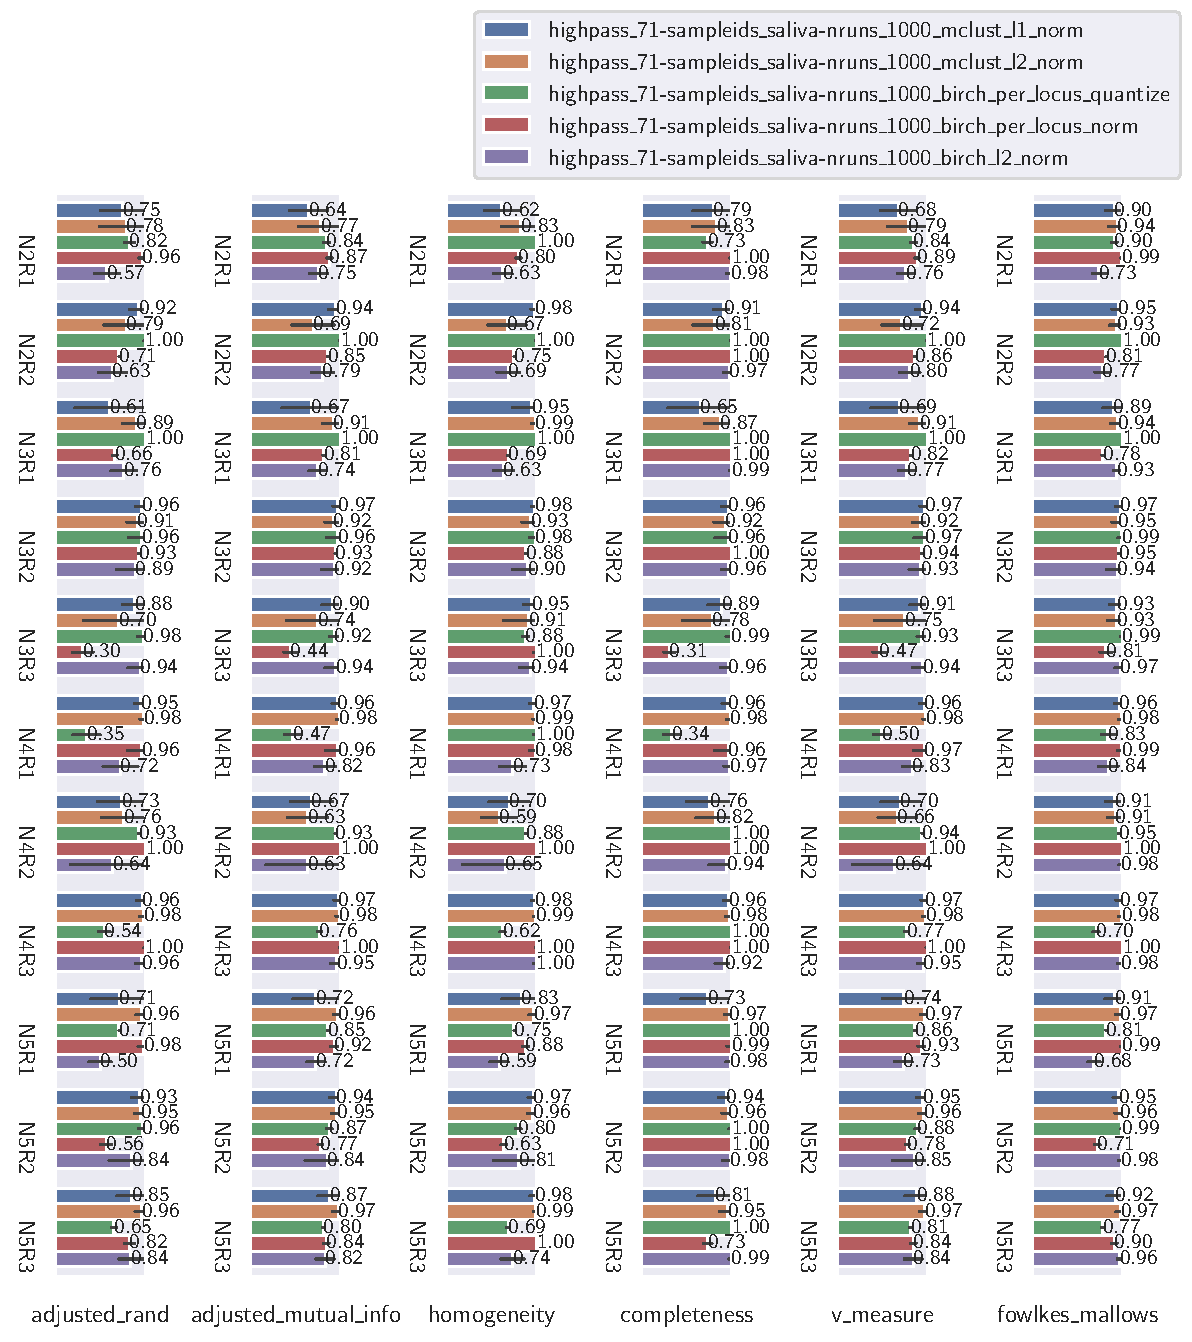
\includegraphics[width=\textwidth]{./figures/clust_comparison/highpass_71-sampleids_saliva-nruns_1000_top_5_clusterers_by_metrics.pdf}
\caption{Top 5 clusterers clustering performance metrics using 1000 trials sampled from EPGs from only saliva samples with high-pass filtering}
\label{fig:highpass_71-sampleids_saliva-nruns_1000_top_5_clusterers_by_metrics}
\end{figure}

\begin{table}[H]
\centering
\maxsizebox{\textwidth}{0.65\textwidth}{
\begin{tabular}{lrr}
\toprule
{} &   mean &    std \\
clusterer                                          &        &        \\
\midrule
hdbscan\_euclidean\_epsilon\_0.0\_eom\_per\_locus\_norm   & 59.08\% & 46.44\% \\
hdbscan\_euclidean\_epsilon\_1.0\_eom\_per\_locus\_norm   & 59.08\% & 46.44\% \\
hdbscan\_euclidean\_epsilon\_0.5\_eom\_per\_locus\_norm   & 59.08\% & 46.44\% \\
hdbscan\_cosine\_epsilon\_0.0\_eom\_per\_locus\_norm      & 58.84\% & 46.75\% \\
hdbscan\_euclidean\_epsilon\_0.0\_eom\_per\_locus\_qua... & 57.91\% & 45.62\% \\
hdbscan\_euclidean\_epsilon\_0.5\_eom\_l2\_norm          & 52.04\% & 41.79\% \\
hdbscan\_euclidean\_epsilon\_0.0\_eom\_l2\_norm          & 52.04\% & 41.79\% \\
hdbscan\_cosine\_epsilon\_0.0\_eom                     & 50.17\% & 40.41\% \\
affinity\_per\_locus\_quantize                        & 49.54\% & 38.19\% \\
hdbscan\_euclidean\_epsilon\_0.5\_leaf\_l2\_norm         & 49.15\% & 39.64\% \\
affinity\_l2\_norm                                   & 48.82\% & 37.70\% \\
mclust\_l2\_norm                                     & 47.68\% & 24.86\% \\
affinity\_per\_locus\_norm                            & 46.21\% & 35.75\% \\
mclust\_l1\_norm                                     & 41.23\% & 20.33\% \\
affinity\_l1\_norm                                   & 38.91\% & 30.07\% \\
optics\_per\_locus\_quantize                          & 35.55\% & 28.93\% \\
hdbscan\_cosine\_epsilon\_0.5\_leaf\_per\_locus\_norm     & 35.12\% & 32.36\% \\
hdbscan\_cosine\_epsilon\_0.5\_eom\_per\_locus\_norm      & 35.12\% & 32.36\% \\
hdbscan\_cosine\_epsilon\_0.0\_eom\_per\_locus\_quantize  & 33.74\% & 27.15\% \\
hdbscan\_euclidean\_epsilon\_0.0\_leaf\_per\_locus\_qu... & 30.83\% & 24.99\% \\
hdbscan\_euclidean\_epsilon\_0.0\_eom\_l1\_norm          & 30.71\% & 27.52\% \\
hdbscan\_euclidean\_epsilon\_0.0\_leaf\_l2\_norm         & 30.69\% & 25.85\% \\
birch\_l2\_norm                                      & 29.69\% & 33.32\% \\
optics\_per\_locus\_norm                              & 29.20\% & 24.32\% \\
birch\_per\_locus\_quantize                           & 26.59\% & 43.92\% \\
\bottomrule
\end{tabular}


}
\caption{Top 25 clusterers by arithmetic mean of percentages of perfect clustering, using admixtures sampled from only saliva EPG data with highpass filter}
\label{table:top_25_not_ensemble_clusterers_by_binomial_confidence_highpass_71-sampleids_saliva-nruns_1000}
\end{table}

\begin{table}[H]
\centering
\maxsizebox{\textwidth}{0.65\textwidth}{
\begin{tabular}{llrrrrrrrrrr}
\toprule
     & {} & \multicolumn{5}{l}{homogeneity} & \multicolumn{5}{l}{completeness} \\
     & clusterer &           1 &       2 &       3 &       4 &       5 &            1 &      2 &      3 &      4 &      5 \\
\midrule
N2R1 & ci\_upp &     100.00\% & 100.00\% &  98.70\% &  98.70\% &   0.38\% &       99.72\% & 99.09\% & 98.86\% & 99.53\% & 66.04\% \\
     & success &     100.00\% & 100.00\% &  98.00\% &  98.00\% &   0.00\% &       99.40\% & 98.50\% & 98.20\% & 99.10\% & 63.10\% \\
     & ci\_low &      99.62\% &  99.62\% &  96.93\% &  96.93\% &   0.00\% &       98.70\% & 97.54\% & 97.17\% & 98.30\% & 60.06\% \\
N2R2 & ci\_upp &       0.38\% & 100.00\% &   0.38\% &  98.86\% & 100.00\% &       52.10\% & 99.38\% & 38.41\% & 99.95\% & 97.30\% \\
     & success &       0.00\% & 100.00\% &   0.00\% &  98.20\% & 100.00\% &       49.00\% & 98.90\% & 35.40\% & 99.80\% & 96.30\% \\
     & ci\_low &       0.00\% &  99.62\% &   0.00\% &  97.17\% &  99.62\% &       45.91\% & 98.04\% & 32.50\% & 99.27\% & 94.94\% \\
N3R1 & ci\_upp &     100.00\% &  99.01\% &   0.38\% & 100.00\% &  99.98\% &       99.09\% & 99.53\% & 47.60\% & 99.53\% & 97.47\% \\
     & success &     100.00\% &  98.40\% &   0.00\% & 100.00\% &  99.90\% &       98.50\% & 99.10\% & 44.50\% & 99.10\% & 96.50\% \\
     & ci\_low &      99.62\% &  97.42\% &   0.00\% &  99.62\% &  99.44\% &       97.54\% & 98.30\% & 41.45\% & 98.30\% & 95.17\% \\
N3R2 & ci\_upp &      99.01\% &   0.38\% & 100.00\% & 100.00\% &   0.38\% &       99.53\% & 52.89\% & 99.38\% & 99.95\% & 53.99\% \\
     & success &      98.40\% &   0.00\% & 100.00\% & 100.00\% &   0.00\% &       99.10\% & 49.80\% & 98.90\% & 99.80\% & 50.90\% \\
     & ci\_low &      97.42\% &   0.00\% &  99.62\% &  99.62\% &   0.00\% &       98.30\% & 46.71\% & 98.04\% & 99.27\% & 47.80\% \\
N3R3 & ci\_upp &       0.38\% &   0.38\% &  64.56\% &  58.06\% & 100.00\% &       38.41\% & 38.41\% & 80.17\% & 82.27\% & 98.30\% \\
     & success &       0.00\% &   0.00\% &  61.60\% &  55.00\% & 100.00\% &       35.40\% & 35.40\% & 77.70\% & 79.90\% & 97.50\% \\
     & ci\_low &       0.00\% &   0.00\% &  58.55\% &  51.90\% &  99.62\% &       32.50\% & 32.50\% & 75.02\% & 77.30\% & 96.34\% \\
N4R1 & ci\_upp &     100.00\% &   0.38\% &   0.38\% &   0.38\% & 100.00\% &       98.78\% & 47.60\% & 52.89\% & 36.18\% & 99.53\% \\
     & success &     100.00\% &   0.00\% &   0.00\% &   0.00\% & 100.00\% &       98.10\% & 44.50\% & 49.80\% & 33.20\% & 99.10\% \\
     & ci\_low &      99.62\% &   0.00\% &   0.00\% &   0.00\% &  99.62\% &       97.05\% & 41.45\% & 46.71\% & 30.35\% & 98.30\% \\
N4R2 & ci\_upp &      98.70\% & 100.00\% & 100.00\% &   0.38\% &  62.01\% &       98.86\% & 98.78\% & 98.78\% & 50.90\% & 79.98\% \\
     & success &      98.00\% & 100.00\% & 100.00\% &   0.00\% &  59.00\% &       98.20\% & 98.10\% & 98.10\% & 47.80\% & 77.50\% \\
     & ci\_low &      96.93\% &  99.62\% &  99.62\% &   0.00\% &  55.92\% &       97.17\% & 97.05\% & 97.05\% & 44.72\% & 74.81\% \\
N4R3 & ci\_upp &     100.00\% &  98.70\% & 100.00\% & 100.00\% &  98.78\% &       99.38\% & 98.86\% & 99.72\% & 99.84\% & 98.38\% \\
     & success &     100.00\% &  98.00\% & 100.00\% & 100.00\% &  98.10\% &       98.90\% & 98.20\% & 99.40\% & 99.60\% & 97.60\% \\
     & ci\_low &      99.62\% &  96.93\% &  99.62\% &  99.62\% &  97.05\% &       98.04\% & 97.17\% & 98.70\% & 98.98\% & 96.45\% \\
N5R1 & ci\_upp &      64.56\% & 100.00\% & 100.00\% &   0.38\% &  98.70\% &       80.17\% & 99.72\% & 99.09\% & 43.88\% & 96.19\% \\
     & success &      61.60\% & 100.00\% & 100.00\% &   0.00\% &  98.00\% &       77.70\% & 99.40\% & 98.50\% & 40.80\% & 95.00\% \\
     & ci\_low &      58.55\% &  99.62\% &  99.62\% &   0.00\% &  96.93\% &       75.02\% & 98.70\% & 97.54\% & 37.79\% & 93.47\% \\
N5R2 & ci\_upp &       0.38\% &   0.38\% &  99.01\% &   0.38\% &   0.38\% &       47.60\% & 52.10\% & 99.53\% & 50.70\% & 44.98\% \\
     & success &       0.00\% &   0.00\% &  98.40\% &   0.00\% &   0.00\% &       44.50\% & 49.00\% & 99.10\% & 47.60\% & 41.90\% \\
     & ci\_low &       0.00\% &   0.00\% &  97.42\% &   0.00\% &   0.00\% &       41.45\% & 45.91\% & 98.30\% & 44.52\% & 38.88\% \\
N5R3 & ci\_upp &       0.38\% &  64.56\% &   0.38\% & 100.00\% &   0.56\% &       52.89\% & 80.17\% & 52.10\% & 99.38\% & 64.66\% \\
     & success &       0.00\% &  61.60\% &   0.00\% & 100.00\% &   0.10\% &       49.80\% & 77.70\% & 49.00\% & 98.90\% & 61.70\% \\
     & ci\_low &       0.00\% &  58.55\% &   0.00\% &  99.62\% &   0.02\% &       46.71\% & 75.02\% & 45.91\% & 98.04\% & 58.65\% \\
\bottomrule
\end{tabular}


}
\caption{Top 5 clusterers clustering percentages of trials where no error occurs using 1000 trials sampled from EPGs from only saliva samples with high-pass filtering}
\label{table:highpass_71-sampleids_saliva-nruns_1000_top_5_clusterers_by_binomial_confidence}
\end{table}

\subsection{Blood Samples Only, without High-Pass Filtering}

\begin{table}[H]
\centering
\maxsizebox{\textwidth}{0.65\textwidth}{
\begin{tabular}{lrr}
\toprule
{} &      mean &       std \\
clusterer                                          &           &           \\
\midrule
mclust\_l1\_norm                                     &  0.793301 &  0.184282 \\
mclust\_l2\_norm                                     &  0.787556 &  0.192270 \\
affinity\_per\_locus\_quantize                        &  0.746803 &  0.229369 \\
birch\_per\_locus\_norm                               &  0.745169 &  0.188504 \\
birch\_per\_locus\_quantize                           &  0.745103 &  0.188918 \\
hdbscan\_euclidean\_epsilon\_0.0\_eom\_per\_locus\_qua... &  0.731431 &  0.270606 \\
hdbscan\_euclidean\_epsilon\_0.0\_eom\_per\_locus\_norm   &  0.726765 &  0.274433 \\
hdbscan\_euclidean\_epsilon\_1.0\_eom\_per\_locus\_norm   &  0.726765 &  0.274433 \\
hdbscan\_euclidean\_epsilon\_0.5\_eom\_per\_locus\_norm   &  0.726765 &  0.274433 \\
affinity\_per\_locus\_norm                            &  0.707305 &  0.254611 \\
meanshift\_per\_locus\_norm                           &  0.668951 &  0.320025 \\
meanshift\_per\_locus\_quantize                       &  0.665926 &  0.316630 \\
affinity\_l2\_norm                                   &  0.665036 &  0.265615 \\
affinity\_l1\_norm                                   &  0.647765 &  0.287850 \\
hdbscan\_euclidean\_epsilon\_0.5\_eom\_l2\_norm          &  0.641548 &  0.334339 \\
hdbscan\_euclidean\_epsilon\_0.0\_eom\_l2\_norm          &  0.641004 &  0.335262 \\
hdbscan\_euclidean\_epsilon\_0.5\_leaf\_l2\_norm         &  0.639636 &  0.333490 \\
hdbscan\_cosine\_epsilon\_0.0\_eom\_per\_locus\_norm      &  0.634984 &  0.338594 \\
hdbscan\_euclidean\_epsilon\_0.0\_eom\_l1\_norm          &  0.634290 &  0.346668 \\
hdbscan\_cosine\_epsilon\_0.0\_eom                     &  0.634045 &  0.336107 \\
hdbscan\_euclidean\_epsilon\_0.0\_leaf\_per\_locus\_qu... &  0.629668 &  0.290115 \\
hdbscan\_cosine\_epsilon\_0.0\_eom\_per\_locus\_quantize  &  0.618541 &  0.323269 \\
hdbscan\_cosine\_epsilon\_0.5\_leaf\_per\_locus\_norm     &  0.608243 &  0.325469 \\
optics\_per\_locus\_norm                              &  0.607149 &  0.301228 \\
hdbscan\_cosine\_epsilon\_0.5\_eom\_per\_locus\_norm      &  0.606929 &  0.327109 \\
\bottomrule
\end{tabular}


}
\caption{Top 25 clusterers by arithmetic mean of clustering metric scores, using admixtures sampled from only blood EPG data without highpass filter}
\label{table:top_25_not_ensemble_clusterers_by_metrics_highpass_0-sampleids_blood-nruns_1000}
\end{table}

\begin{figure}[H]
\centering
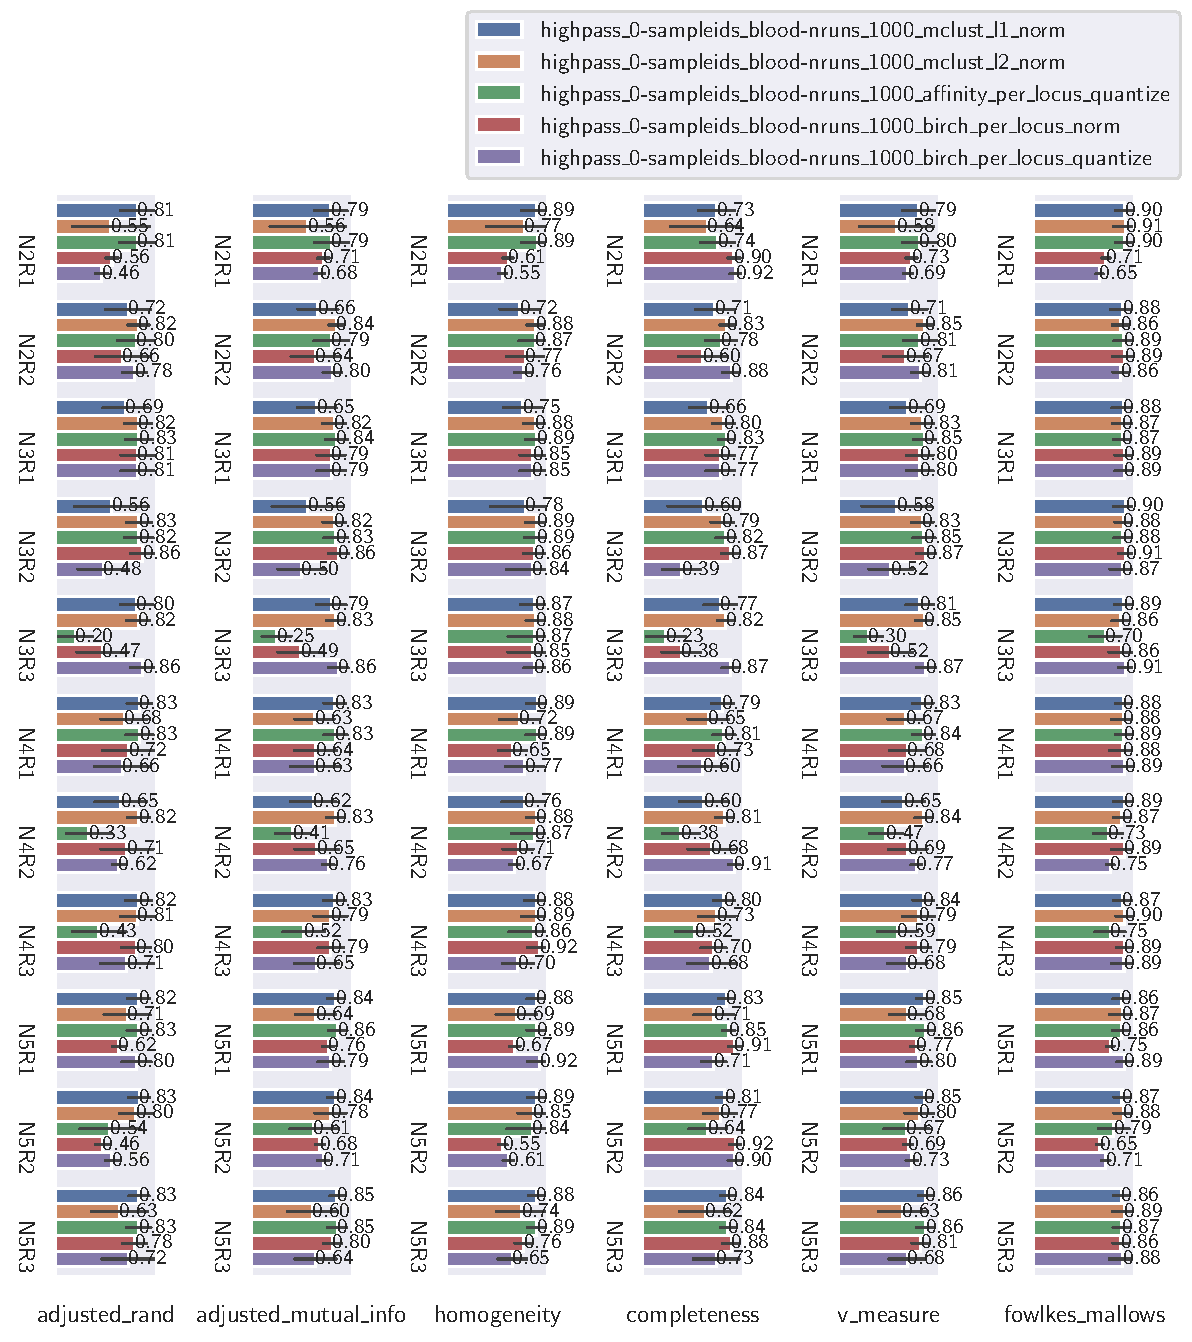
\includegraphics[width=\textwidth]{./figures/clust_comparison/highpass_0-sampleids_blood-nruns_1000_top_5_clusterers_by_metrics.pdf}
\caption{Top 5 clusterers clustering performance metrics using 1000 trials sampled from EPGs from only blood samples without high-pass filtering}
\label{fig:highpass_0-sampleids_blood-nruns_1000_top_5_clusterers_by_metrics}
\end{figure}

\begin{table}[H]
\centering
\maxsizebox{\textwidth}{0.65\textwidth}{
\begin{tabular}{lrr}
\toprule
{} &  mean &    std \\
clusterer                                          &       &        \\
\midrule
mclust\_l2\_norm                                     & 9.10\% & 10.15\% \\
mclust\_l1\_norm                                     & 8.92\% &  9.30\% \\
hdbscan\_euclidean\_epsilon\_0.0\_eom\_per\_locus\_qua... & 4.98\% &  7.95\% \\
hdbscan\_euclidean\_epsilon\_0.5\_eom\_per\_locus\_norm   & 4.90\% &  7.89\% \\
hdbscan\_euclidean\_epsilon\_0.0\_eom\_per\_locus\_norm   & 4.90\% &  7.89\% \\
hdbscan\_euclidean\_epsilon\_1.0\_eom\_per\_locus\_norm   & 4.90\% &  7.89\% \\
affinity\_per\_locus\_quantize                        & 3.75\% &  4.93\% \\
affinity\_per\_locus\_norm                            & 3.61\% &  5.16\% \\
birch\_per\_locus\_norm                               & 3.39\% &  5.53\% \\
birch\_per\_locus\_quantize                           & 3.35\% &  5.47\% \\
birch\_l2\_norm                                      & 3.07\% &  3.95\% \\
hdbscan\_euclidean\_epsilon\_0.0\_leaf\_per\_locus\_qu... & 2.49\% &  4.09\% \\
meanshift\_per\_locus\_norm                           & 2.10\% &  1.82\% \\
hdbscan\_euclidean\_epsilon\_0.0\_leaf\_per\_locus\_norm  & 1.99\% &  3.50\% \\
hdbscan\_euclidean\_epsilon\_0.5\_leaf\_per\_locus\_norm  & 1.99\% &  3.50\% \\
hdbscan\_euclidean\_epsilon\_1.0\_leaf\_per\_locus\_norm  & 1.99\% &  3.50\% \\
hdbscan\_euclidean\_epsilon\_0.0\_eom\_l2\_norm          & 1.75\% &  2.73\% \\
hdbscan\_euclidean\_epsilon\_0.5\_eom\_l2\_norm          & 1.75\% &  2.73\% \\
hdbscan\_cosine\_epsilon\_0.0\_eom                     & 1.75\% &  2.73\% \\
hdbscan\_euclidean\_epsilon\_0.5\_leaf\_l2\_norm         & 1.72\% &  2.70\% \\
affinity\_l2\_norm                                   & 1.72\% &  2.81\% \\
hdbscan\_euclidean\_epsilon\_0.0\_eom\_l1\_norm          & 1.68\% &  2.32\% \\
optics\_per\_locus\_quantize                          & 1.67\% &  2.79\% \\
hdbscan\_cosine\_epsilon\_0.0\_eom\_per\_locus\_norm      & 1.63\% &  2.56\% \\
hdbscan\_cosine\_epsilon\_0.5\_eom\_per\_locus\_norm      & 1.54\% &  2.57\% \\
\bottomrule
\end{tabular}


}
\caption{Top 25 clusterers by arithmetic mean of percentages of perfect clustering, using admixtures sampled from only blood EPG data without highpass filter}
\label{table:top_25_not_ensemble_clusterers_by_binomial_confidence_highpass_0-sampleids_blood-nruns_1000}
\end{table}

\begin{table}[H]
\centering
\maxsizebox{\textwidth}{0.65\textwidth}{
\begin{tabular}{llrrrrrrrrrr}
\toprule
     & {} & \multicolumn{5}{l}{homogeneity} & \multicolumn{5}{l}{completeness} \\
     & clusterer &           1 &      2 &      3 &      4 &      5 &            1 &      2 &      3 &      4 &      5 \\
\midrule
N2R1 & ci\_upp &      69.84\% & 40.95\% &  0.38\% &  4.37\% & 48.00\% &       50.30\% & 21.44\% & 23.22\% &  1.83\% & 29.01\% \\
     & success &      67.00\% & 37.90\% &  0.00\% &  3.10\% & 44.90\% &       47.20\% & 18.90\% & 20.60\% &  1.00\% & 26.20\% \\
     & ci\_low &      64.03\% & 34.94\% &  0.00\% &  2.19\% & 41.84\% &       44.12\% & 16.59\% & 18.21\% &  0.54\% & 23.57\% \\
N2R2 & ci\_upp &       1.02\% & 16.61\% &  2.21\% & 33.53\% & 15.01\% &        0.73\% & 16.08\% & 26.95\% & 23.94\% &  7.65\% \\
     & success &       0.40\% & 14.30\% &  1.30\% & 30.60\% & 12.80\% &        0.20\% & 13.80\% & 24.20\% & 21.30\% &  6.00\% \\
     & ci\_low &       0.16\% & 12.27\% &  0.76\% & 27.82\% & 10.87\% &        0.05\% & 11.80\% & 21.65\% & 18.87\% &  4.69\% \\
N3R1 & ci\_upp &       8.64\% & 23.53\% & 12.12\% &  1.44\% & 12.23\% &        4.83\% & 13.41\% &  7.54\% &  0.56\% &  7.54\% \\
     & success &       6.90\% & 20.90\% & 10.10\% &  0.70\% & 10.20\% &        3.50\% & 11.30\% &  5.90\% &  0.10\% &  5.90\% \\
     & ci\_low &       5.49\% & 18.49\% &  8.38\% &  0.34\% &  8.47\% &        2.53\% &  9.48\% &  4.60\% &  0.02\% &  4.60\% \\
N3R2 & ci\_upp &      10.61\% & 67.01\% & 48.30\% & 22.49\% & 33.53\% &        6.64\% & 44.38\% & 29.42\% & 18.61\% & 23.94\% \\
     & success &       8.70\% & 64.10\% & 45.20\% & 19.90\% & 30.60\% &        5.10\% & 41.30\% & 26.60\% & 16.20\% & 21.30\% \\
     & ci\_low &       7.11\% & 61.08\% & 42.14\% & 17.54\% & 27.82\% &        3.90\% & 38.29\% & 23.95\% & 14.05\% & 18.87\% \\
N3R3 & ci\_upp &       2.95\% & 29.84\% &  5.29\% &  0.56\% &  0.56\% &        1.83\% & 20.08\% &  2.34\% & 19.24\% & 19.24\% \\
     & success &       1.90\% & 27.00\% &  3.90\% &  0.10\% &  0.10\% &        1.00\% & 17.60\% &  1.40\% & 16.80\% & 16.80\% \\
     & ci\_low &       1.22\% & 24.34\% &  2.87\% &  0.02\% &  0.02\% &        0.54\% & 15.36\% &  0.84\% & 14.61\% & 14.61\% \\
N4R1 & ci\_upp &      20.19\% & 11.26\% & 14.91\% & 12.23\% &  0.38\% &       12.45\% &  6.19\% &  7.98\% &  7.54\% & 18.82\% \\
     & success &      17.70\% &  9.30\% & 12.70\% & 10.20\% &  0.00\% &       10.40\% &  4.70\% &  6.30\% &  5.90\% & 16.40\% \\
     & ci\_low &      15.46\% &  7.65\% & 10.78\% &  8.47\% &  0.00\% &        8.66\% &  3.55\% &  4.95\% &  4.60\% & 14.23\% \\
N4R2 & ci\_upp &       3.78\% & 35.67\% &  4.25\% &  0.38\% &  4.37\% &        2.46\% & 19.56\% &  1.96\% & 18.82\% &  1.83\% \\
     & success &       2.60\% & 32.70\% &  3.00\% &  0.00\% &  3.10\% &        1.50\% & 17.10\% &  1.10\% & 16.40\% &  1.00\% \\
     & ci\_low &       1.78\% & 29.86\% &  2.11\% &  0.00\% &  2.19\% &        0.91\% & 14.89\% &  0.62\% & 14.23\% &  0.54\% \\
N4R3 & ci\_upp &      41.35\% &  9.19\% & 33.01\% & 48.00\% &  5.74\% &       22.49\% &  4.83\% & 31.17\% & 29.01\% &  2.58\% \\
     & success &      38.30\% &  7.40\% & 30.10\% & 44.90\% &  4.30\% &       19.90\% &  3.50\% & 28.30\% & 26.20\% &  1.60\% \\
     & ci\_low &      35.34\% &  5.94\% & 27.34\% & 41.84\% &  3.21\% &       17.54\% &  2.53\% & 25.60\% & 23.57\% &  0.99\% \\
N5R1 & ci\_upp &      13.95\% &  3.31\% &  1.70\% &  0.38\% &  0.38\% &       16.82\% &  1.83\% &  0.38\% & 18.19\% & 18.19\% \\
     & success &      11.80\% &  2.20\% &  0.90\% &  0.00\% &  0.00\% &       14.50\% &  1.00\% &  0.00\% & 15.80\% & 15.80\% \\
     & ci\_low &       9.95\% &  1.46\% &  0.47\% &  0.00\% &  0.00\% &       12.45\% &  0.54\% &  0.00\% & 13.67\% & 13.67\% \\
N5R2 & ci\_upp &      29.12\% &  3.66\% &  0.38\% &  5.74\% & 22.49\% &       20.92\% &  1.83\% & 22.28\% &  2.58\% & 18.61\% \\
     & success &      26.30\% &  2.50\% &  0.00\% &  4.30\% & 19.90\% &       18.40\% &  1.00\% & 19.70\% &  1.60\% & 16.20\% \\
     & ci\_low &      23.67\% &  1.70\% &  0.00\% &  3.21\% & 17.54\% &       16.12\% &  0.54\% & 17.35\% &  0.99\% & 14.05\% \\
N5R3 & ci\_upp &      35.57\% &  1.30\% & 22.70\% & 15.01\% &  1.44\% &       22.49\% &  0.73\% & 18.19\% &  7.65\% &  0.56\% \\
     & success &      32.60\% &  0.60\% & 20.10\% & 12.80\% &  0.70\% &       19.90\% &  0.20\% & 15.80\% &  6.00\% &  0.10\% \\
     & ci\_low &      29.77\% &  0.28\% & 17.73\% & 10.87\% &  0.34\% &       17.54\% &  0.05\% & 13.67\% &  4.69\% &  0.02\% \\
\bottomrule
\end{tabular}


}
\caption{Top 5 clusterers clustering percentages of trials where no error occurs using 1000 trials sampled from EPGs from only blood samples without high-pass filtering}
\label{table:highpass_0-sampleids_blood-nruns_1000_top_5_clusterers_by_binomial_confidence}
\end{table}

\subsection{Blood Samples Only, with High-Pass Filtering}

\begin{table}[H]
\centering
\maxsizebox{\textwidth}{0.65\textwidth}{
\begin{tabular}{lrr}
\toprule
{} &      mean &       std \\
clusterer                                          &           &           \\
\midrule
mclust\_l1\_norm                                     &  0.960895 &  0.098183 \\
mclust\_l2\_norm                                     &  0.953501 &  0.107068 \\
birch\_per\_locus\_quantize                           &  0.849550 &  0.173975 \\
affinity\_per\_locus\_quantize                        &  0.844791 &  0.250112 \\
birch\_per\_locus\_norm                               &  0.842968 &  0.184070 \\
affinity\_per\_locus\_norm                            &  0.792776 &  0.294350 \\
affinity\_l1\_norm                                   &  0.791961 &  0.290986 \\
affinity\_l2\_norm                                   &  0.787894 &  0.297917 \\
birch\_l2\_norm                                      &  0.779446 &  0.227425 \\
hdbscan\_euclidean\_epsilon\_0.0\_eom\_per\_locus\_qua... &  0.777033 &  0.348583 \\
meanshift\_per\_locus\_norm                           &  0.768090 &  0.356926 \\
hdbscan\_euclidean\_epsilon\_0.5\_eom\_l2\_norm          &  0.767799 &  0.354855 \\
hdbscan\_euclidean\_epsilon\_0.0\_eom\_l2\_norm          &  0.767208 &  0.356015 \\
hdbscan\_euclidean\_epsilon\_0.5\_leaf\_l2\_norm         &  0.765516 &  0.354534 \\
meanshift\_l2\_norm                                  &  0.765354 &  0.356738 \\
hdbscan\_cosine\_epsilon\_0.0\_eom                     &  0.764884 &  0.356171 \\
hdbscan\_euclidean\_epsilon\_0.0\_eom\_l1\_norm          &  0.763600 &  0.359556 \\
hdbscan\_cosine\_epsilon\_0.0\_eom\_per\_locus\_norm      &  0.759901 &  0.362087 \\
hdbscan\_euclidean\_epsilon\_0.0\_eom\_per\_locus\_norm   &  0.757295 &  0.366148 \\
hdbscan\_euclidean\_epsilon\_1.0\_eom\_per\_locus\_norm   &  0.757295 &  0.366148 \\
hdbscan\_euclidean\_epsilon\_0.5\_eom\_per\_locus\_norm   &  0.757295 &  0.366148 \\
meanshift\_l1\_norm                                  &  0.754057 &  0.354813 \\
meanshift\_per\_locus\_quantize                       &  0.748134 &  0.354944 \\
hdbscan\_cosine\_epsilon\_0.0\_eom\_per\_locus\_quantize  &  0.745206 &  0.349276 \\
hdbscan\_cosine\_epsilon\_0.5\_leaf\_per\_locus\_norm     &  0.722215 &  0.352943 \\
\bottomrule
\end{tabular}


}
\caption{Top 25 clusterers by arithmetic mean of clustering metric scores, using admixtures sampled from only blood EPG data with highpass filter}
\label{table:top_25_not_ensemble_clusterers_by_metrics_highpass_71-sampleids_blood-nruns_1000}
\end{table}

\begin{figure}[H]
\centering
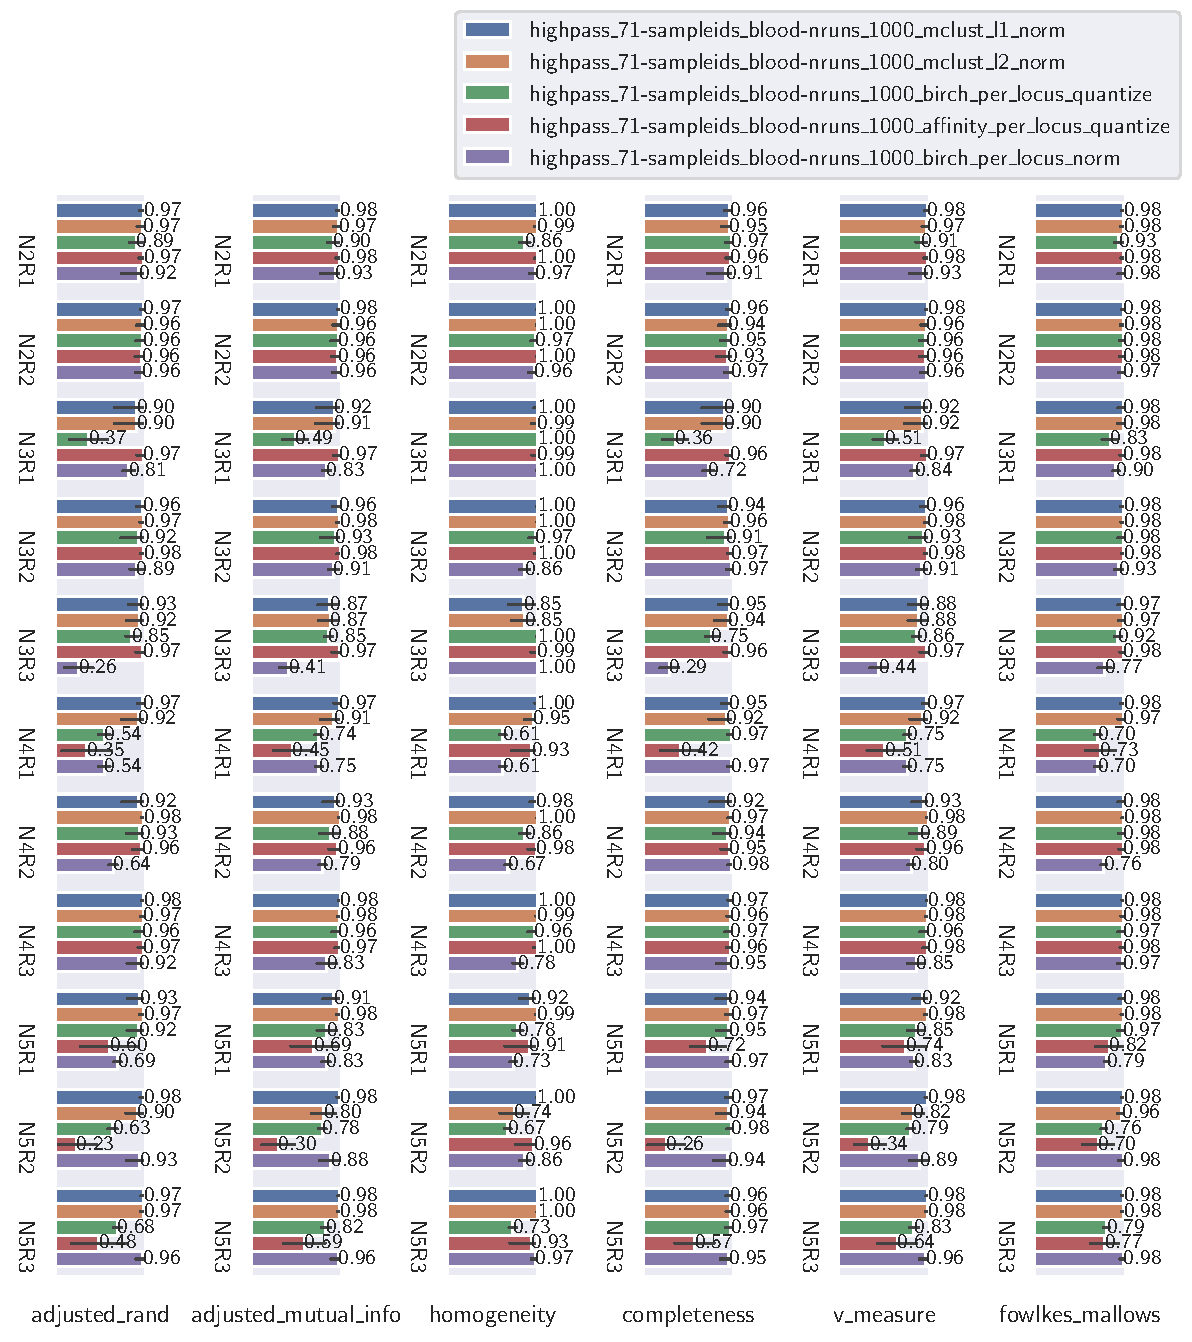
\includegraphics[width=\textwidth]{./figures/clust_comparison/highpass_71-sampleids_blood-nruns_1000_top_5_clusterers_by_metrics.pdf}
\caption{Top 5 clusterers clustering performance metrics using 1000 trials sampled from EPGs from only blood samples with high-pass filtering}
\label{fig:highpass_71-sampleids_blood-nruns_1000_top_5_clusterers_by_metrics}
\end{figure}

\begin{table}[H]
\centering
\maxsizebox{\textwidth}{0.65\textwidth}{
\begin{tabular}{lrr}
\toprule
{} &   mean &    std \\
clusterer                                          &        &        \\
\midrule
mclust\_l1\_norm                                     & 64.13\% & 12.62\% \\
mclust\_l2\_norm                                     & 59.02\% & 18.32\% \\
affinity\_per\_locus\_quantize                        & 39.18\% & 29.74\% \\
affinity\_per\_locus\_norm                            & 39.05\% & 30.77\% \\
affinity\_l1\_norm                                   & 38.79\% & 30.49\% \\
affinity\_l2\_norm                                   & 38.67\% & 30.44\% \\
hdbscan\_euclidean\_epsilon\_0.0\_eom\_per\_locus\_norm   & 36.66\% & 29.52\% \\
hdbscan\_euclidean\_epsilon\_0.5\_eom\_per\_locus\_norm   & 36.66\% & 29.52\% \\
hdbscan\_euclidean\_epsilon\_1.0\_eom\_per\_locus\_norm   & 36.66\% & 29.52\% \\
hdbscan\_cosine\_epsilon\_0.0\_eom\_per\_locus\_norm      & 36.57\% & 29.50\% \\
hdbscan\_euclidean\_epsilon\_0.0\_eom\_per\_locus\_qua... & 36.15\% & 29.37\% \\
hdbscan\_euclidean\_epsilon\_0.0\_eom\_l2\_norm          & 36.15\% & 29.42\% \\
hdbscan\_euclidean\_epsilon\_0.5\_eom\_l2\_norm          & 36.15\% & 29.42\% \\
hdbscan\_cosine\_epsilon\_0.0\_eom                     & 36.15\% & 29.42\% \\
hdbscan\_euclidean\_epsilon\_0.0\_eom\_l1\_norm          & 36.06\% & 29.25\% \\
hdbscan\_euclidean\_epsilon\_0.5\_leaf\_l2\_norm         & 35.25\% & 28.76\% \\
hdbscan\_cosine\_epsilon\_0.0\_eom\_per\_locus\_quantize  & 30.66\% & 25.33\% \\
meanshift\_per\_locus\_norm                           & 30.12\% & 21.63\% \\
meanshift\_l2\_norm                                  & 28.52\% & 21.48\% \\
hdbscan\_cosine\_epsilon\_0.5\_eom\_per\_locus\_norm      & 26.82\% & 24.40\% \\
hdbscan\_cosine\_epsilon\_0.5\_leaf\_per\_locus\_norm     & 26.82\% & 24.40\% \\
birch\_l2\_norm                                      & 23.59\% & 28.61\% \\
meanshift\_l1\_norm                                  & 22.28\% & 18.21\% \\
meanshift\_per\_locus\_quantize                       & 22.00\% & 19.25\% \\
birch\_per\_locus\_norm                               & 21.45\% & 35.42\% \\
\bottomrule
\end{tabular}


}
\caption{Top 25 clusterers by arithmetic mean of percentages of perfect clustering, using admixtures sampled from only blood EPG data with highpass filter}
\label{table:top_25_not_ensemble_clusterers_by_binomial_confidence_highpass_71-sampleids_blood-nruns_1000}
\end{table}

\begin{table}[H]
\centering
\maxsizebox{\textwidth}{0.65\textwidth}{
\begin{tabular}{llrrrrrrrrrr}
\toprule
     & {} & \multicolumn{5}{l}{homogeneity} & \multicolumn{5}{l}{completeness} \\
     & clusterer &           1 &      2 &      3 &      4 &      5 &            1 &      2 &      3 &      4 &      5 \\
\midrule
N2R1 & ci\_upp &      98.62\% & 94.69\% & 95.93\% & 97.13\% & 94.96\% &       70.33\% & 78.74\% & 68.38\% &  2.34\% & 75.56\% \\
     & success &      97.90\% & 93.30\% & 94.70\% & 96.10\% & 93.60\% &       67.50\% & 76.20\% & 65.50\% &  1.40\% & 72.90\% \\
     & ci\_low &      96.81\% & 91.58\% & 93.13\% & 94.71\% & 91.91\% &       64.53\% & 73.46\% & 62.50\% &  0.84\% & 70.06\% \\
N2R2 & ci\_upp &      92.17\% & 99.24\% & 99.66\% & 92.80\% & 83.41\% &       55.58\% & 78.45\% & 74.50\% & 52.69\% &  7.31\% \\
     & success &      90.50\% & 98.70\% & 99.30\% & 91.20\% & 81.10\% &       52.50\% & 75.90\% & 71.80\% & 49.60\% &  5.70\% \\
     & ci\_low &      88.52\% & 97.79\% & 98.56\% & 89.28\% & 78.56\% &       49.40\% & 73.15\% & 68.93\% & 46.51\% &  4.43\% \\
N3R1 & ci\_upp &      99.90\% & 99.66\% & 97.39\% & 95.22\% & 91.53\% &       86.61\% & 86.80\% & 57.37\% & 75.37\% &  4.02\% \\
     & success &      99.70\% & 99.30\% & 96.40\% & 93.90\% & 89.80\% &       84.50\% & 84.70\% & 54.30\% & 72.70\% &  2.80\% \\
     & ci\_low &      99.12\% & 98.56\% & 95.06\% & 92.24\% & 87.77\% &       82.13\% & 82.34\% & 51.20\% & 69.86\% &  1.94\% \\
N3R2 & ci\_upp &      99.16\% & 98.62\% & 97.39\% & 98.86\% & 98.94\% &       78.35\% & 70.62\% & 51.60\% & 69.36\% & 69.36\% \\
     & success &      98.60\% & 97.90\% & 96.40\% & 98.20\% & 98.30\% &       75.80\% & 67.80\% & 48.50\% & 66.50\% & 66.50\% \\
     & ci\_low &      97.66\% & 96.81\% & 95.06\% & 97.17\% & 97.29\% &       73.05\% & 64.84\% & 45.41\% & 63.52\% & 63.52\% \\
N3R3 & ci\_upp &      54.49\% & 48.10\% & 98.54\% & 96.45\% & 95.05\% &       86.61\% & 87.83\% & 68.77\% & 68.77\% &  3.90\% \\
     & success &      51.40\% & 45.00\% & 97.80\% & 95.30\% & 93.70\% &       84.50\% & 85.80\% & 65.90\% & 65.90\% &  2.70\% \\
     & ci\_low &      48.30\% & 41.94\% & 96.69\% & 93.81\% & 92.02\% &       82.13\% & 83.50\% & 62.91\% & 62.91\% &  1.86\% \\
N4R1 & ci\_upp &      96.45\% & 77.68\% & 91.07\% & 99.84\% & 92.44\% &       78.45\% & 86.42\% &  7.54\% & 74.40\% & 53.39\% \\
     & success &      95.30\% & 75.10\% & 89.30\% & 99.60\% & 90.80\% &       75.90\% & 84.30\% &  5.90\% & 71.70\% & 50.30\% \\
     & ci\_low &      93.81\% & 72.33\% & 87.23\% & 98.98\% & 88.85\% &       73.15\% & 81.91\% &  4.60\% & 68.83\% & 47.21\% \\
N4R2 & ci\_upp &      89.13\% & 95.05\% & 95.13\% & 91.98\% & 99.79\% &       86.42\% & 53.39\% & 74.98\% &  5.74\% & 70.91\% \\
     & success &      87.20\% & 93.70\% & 93.80\% & 90.30\% & 99.50\% &       84.30\% & 50.30\% & 72.30\% &  4.30\% & 68.10\% \\
     & ci\_low &      84.99\% & 92.02\% & 92.13\% & 88.31\% & 98.83\% &       81.91\% & 47.21\% & 69.44\% &  3.21\% & 65.15\% \\
N4R3 & ci\_upp &      96.88\% & 87.73\% & 92.44\% & 97.72\% & 95.57\% &       53.29\% & 55.48\% & 52.00\% & 52.00\% & 68.58\% \\
     & success &      95.80\% & 85.70\% & 90.80\% & 96.80\% & 94.30\% &       50.20\% & 52.40\% & 48.90\% & 48.90\% & 65.70\% \\
     & ci\_low &      94.37\% & 83.39\% & 88.85\% & 95.52\% & 92.69\% &       47.11\% & 49.30\% & 45.81\% & 45.81\% & 62.70\% \\
N5R1 & ci\_upp &      71.89\% & 92.35\% & 83.31\% & 82.74\% & 88.20\% &       87.64\% & 71.60\% & 14.59\% &  9.41\% &  5.51\% \\
     & success &      69.10\% & 90.70\% & 81.00\% & 80.40\% & 86.20\% &       85.60\% & 68.80\% & 12.40\% &  7.60\% &  4.10\% \\
     & ci\_low &      66.17\% & 88.74\% & 78.45\% & 77.83\% & 83.92\% &       83.29\% & 65.86\% & 10.50\% &  6.11\% &  3.04\% \\
N5R2 & ci\_upp &      95.66\% & 25.71\% & 96.36\% & 97.56\% & 97.56\% &       71.89\% & 86.80\% &  5.51\% & 57.86\% & 52.20\% \\
     & success &      94.40\% & 23.00\% & 95.20\% & 96.60\% & 96.60\% &       69.10\% & 84.70\% &  4.10\% & 54.80\% & 49.10\% \\
     & ci\_low &      92.80\% & 20.50\% & 93.69\% & 95.29\% & 95.29\% &       66.17\% & 82.34\% &  3.04\% & 51.70\% & 46.01\% \\
N5R3 & ci\_upp &      97.30\% & 96.19\% & 86.89\% & 87.73\% & 98.22\% &       59.05\% & 59.05\% &  9.19\% &  6.64\% & 59.05\% \\
     & success &      96.30\% & 95.00\% & 84.80\% & 85.70\% & 97.40\% &       56.00\% & 56.00\% &  7.40\% &  5.10\% & 56.00\% \\
     & ci\_low &      94.94\% & 93.47\% & 82.44\% & 83.39\% & 96.22\% &       52.91\% & 52.91\% &  5.94\% &  3.90\% & 52.91\% \\
\bottomrule
\end{tabular}


}
\caption{Top 5 clusterers clustering percentages of trials where no error occurs using 1000 trials sampled from EPGs from only blood samples with high-pass filtering}
\label{table:highpass_71-sampleids_blood-nruns_1000_top_5_clusterers_by_binomial_confidence}
\end{table}

\subsection{All Samples, without High-Pass Filtering}

\begin{table}[H]
\centering
\maxsizebox{\textwidth}{0.65\textwidth}{
\begin{tabular}{lrr}
\toprule
{} &      mean &       std \\
clusterer                                          &           &           \\
\midrule
birch\_per\_locus\_quantize                           &  0.641797 &  0.211116 \\
birch\_per\_locus\_norm                               &  0.641290 &  0.211306 \\
mclust\_l1\_norm                                     &  0.632317 &  0.234902 \\
mclust\_l2\_norm                                     &  0.628675 &  0.240790 \\
affinity\_per\_locus\_quantize                        &  0.626572 &  0.227781 \\
affinity\_l2\_norm                                   &  0.616125 &  0.234093 \\
hdbscan\_euclidean\_epsilon\_0.0\_eom\_per\_locus\_qua... &  0.606724 &  0.259711 \\
hdbscan\_euclidean\_epsilon\_0.5\_eom\_per\_locus\_norm   &  0.606178 &  0.262164 \\
hdbscan\_euclidean\_epsilon\_0.0\_eom\_per\_locus\_norm   &  0.606178 &  0.262164 \\
hdbscan\_euclidean\_epsilon\_1.0\_eom\_per\_locus\_norm   &  0.606178 &  0.262164 \\
affinity\_per\_locus\_norm                            &  0.601773 &  0.234468 \\
meanshift\_per\_locus\_norm                           &  0.588258 &  0.305518 \\
meanshift\_per\_locus\_quantize                       &  0.583719 &  0.298994 \\
hdbscan\_cosine\_epsilon\_0.0\_eom\_per\_locus\_norm      &  0.579221 &  0.314593 \\
hdbscan\_euclidean\_epsilon\_0.5\_eom\_l2\_norm          &  0.576326 &  0.308595 \\
hdbscan\_euclidean\_epsilon\_0.0\_eom\_l2\_norm          &  0.575876 &  0.309118 \\
hdbscan\_cosine\_epsilon\_0.0\_eom                     &  0.569691 &  0.308828 \\
hdbscan\_cosine\_epsilon\_0.0\_eom\_per\_locus\_quantize  &  0.567093 &  0.303365 \\
hdbscan\_euclidean\_epsilon\_0.5\_leaf\_l2\_norm         &  0.563626 &  0.308553 \\
hdbscan\_cosine\_epsilon\_0.5\_eom\_per\_locus\_norm      &  0.562861 &  0.307425 \\
hdbscan\_cosine\_epsilon\_0.5\_leaf\_per\_locus\_norm     &  0.562268 &  0.305130 \\
affinity\_l1\_norm                                   &  0.561750 &  0.265127 \\
hdbscan\_euclidean\_epsilon\_0.0\_eom\_l1\_norm          &  0.536147 &  0.311479 \\
hdbscan\_euclidean\_epsilon\_0.0\_leaf\_per\_locus\_qu... &  0.524716 &  0.262260 \\
optics\_l2\_norm                                     &  0.524296 &  0.305004 \\
\bottomrule
\end{tabular}


}
\caption{Top 25 clusterers by arithmetic mean of clustering metric scores, using admixtures sampled from all EPG data without highpass filter}
\label{table:top_25_not_ensemble_clusterers_by_metrics_highpass_0-sampleids_all-nruns_1000}
\end{table}

\begin{figure}[H]
\centering
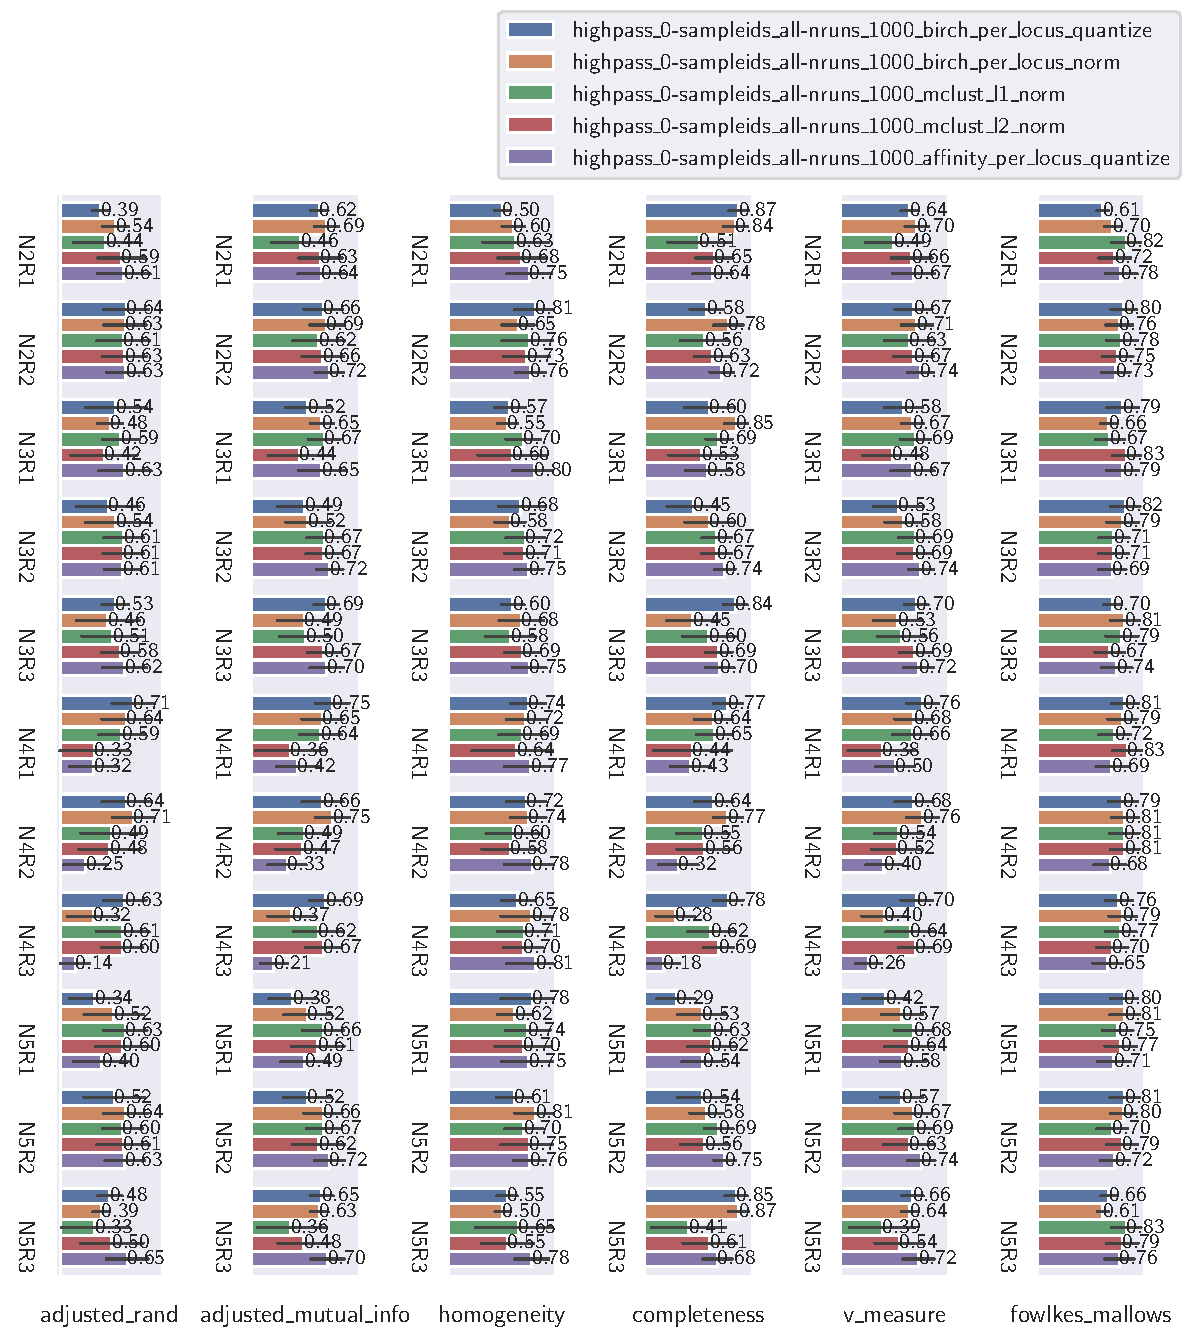
\includegraphics[width=\textwidth]{./figures/clust_comparison/highpass_0-sampleids_all-nruns_1000_top_5_clusterers_by_metrics.pdf}
\caption{Top 5 clusterers clustering performance metrics using 1000 trials sampled from all EPGs without high-pass filtering}
\label{fig:highpass_0-sampleids_all-nruns_1000_top_5_clusterers_by_metrics}
\end{figure}

\begin{table}[H]
\centering
\maxsizebox{\textwidth}{0.65\textwidth}{
\begin{tabular}{lrr}
\toprule
{} &  mean &   std \\
clusterer                                          &       &       \\
\midrule
mclust\_l2\_norm                                     & 3.09\% & 4.12\% \\
mclust\_l1\_norm                                     & 2.97\% & 3.75\% \\
meanshift\_per\_locus\_norm                           & 2.66\% & 2.49\% \\
hdbscan\_euclidean\_epsilon\_1.0\_eom\_per\_locus\_norm   & 2.39\% & 4.63\% \\
hdbscan\_euclidean\_epsilon\_0.0\_eom\_per\_locus\_norm   & 2.39\% & 4.63\% \\
hdbscan\_euclidean\_epsilon\_0.5\_eom\_per\_locus\_norm   & 2.39\% & 4.63\% \\
hdbscan\_euclidean\_epsilon\_0.0\_eom\_per\_locus\_qua... & 2.23\% & 4.47\% \\
meanshift\_per\_locus\_quantize                       & 1.91\% & 1.98\% \\
birch\_per\_locus\_quantize                           & 1.78\% & 2.88\% \\
birch\_per\_locus\_norm                               & 1.73\% & 2.79\% \\
birch\_l2\_norm                                      & 1.25\% & 1.63\% \\
affinity\_per\_locus\_norm                            & 1.22\% & 2.13\% \\
affinity\_per\_locus\_quantize                        & 1.18\% & 1.97\% \\
optics\_per\_locus\_quantize                          & 1.18\% & 2.40\% \\
optics\_per\_locus\_norm                              & 1.14\% & 2.16\% \\
hdbscan\_euclidean\_epsilon\_0.0\_leaf\_per\_locus\_qu... & 0.99\% & 2.03\% \\
hdbscan\_euclidean\_epsilon\_1.0\_leaf\_per\_locus\_norm  & 0.95\% & 1.79\% \\
hdbscan\_euclidean\_epsilon\_0.0\_leaf\_per\_locus\_norm  & 0.95\% & 1.79\% \\
hdbscan\_euclidean\_epsilon\_0.5\_leaf\_per\_locus\_norm  & 0.95\% & 1.79\% \\
hdbscan\_euclidean\_epsilon\_0.0\_eom\_l2\_norm          & 0.81\% & 1.41\% \\
hdbscan\_euclidean\_epsilon\_0.5\_eom\_l2\_norm          & 0.81\% & 1.41\% \\
hdbscan\_cosine\_epsilon\_0.0\_eom                     & 0.80\% & 1.38\% \\
hdbscan\_euclidean\_epsilon\_0.5\_leaf\_l2\_norm         & 0.74\% & 1.27\% \\
hdbscan\_cosine\_epsilon\_0.0\_eom\_per\_locus\_quantize  & 0.74\% & 1.31\% \\
hdbscan\_euclidean\_epsilon\_1.0\_eom\_l2\_norm          & 0.74\% & 1.42\% \\
\bottomrule
\end{tabular}


}
\caption{Top 25 clusterers by arithmetic mean of percentages of perfect clustering, using admixtures sampled from all EPG data without highpass filter}
\label{table:top_25_not_ensemble_clusterers_by_binomial_confidence_highpass_0-sampleids_all-nruns_1000}
\end{table}

\begin{table}[H]
\centering
\maxsizebox{\textwidth}{0.65\textwidth}{
\begin{tabular}{llrrrrrrrrrr}
\toprule
     & {} & \multicolumn{5}{l}{homogeneity} & \multicolumn{5}{l}{completeness} \\
     & clusterer &           1 &      2 &      3 &      4 &      5 &            1 &      2 &      3 &      4 &      5 \\
\midrule
N2R1 & ci\_upp &       2.46\% & 23.63\% & 21.23\% &  3.66\% &  0.88\% &        1.57\% & 19.66\% &  8.86\% &  4.71\% &  1.44\% \\
     & success &       1.50\% & 21.00\% & 18.70\% &  2.50\% &  0.30\% &        0.80\% & 17.20\% &  7.10\% &  3.40\% &  0.70\% \\
     & ci\_low &       0.91\% & 18.59\% & 16.40\% &  1.70\% &  0.10\% &        0.41\% & 14.99\% &  5.67\% &  2.44\% &  0.34\% \\
N2R2 & ci\_upp &       4.48\% & 27.57\% & 27.16\% &  0.38\% &  6.64\% &        1.57\% &  9.30\% &  7.76\% &  0.38\% &  4.83\% \\
     & success &       3.20\% & 24.80\% & 24.40\% &  0.00\% &  5.10\% &        0.80\% &  7.50\% &  6.10\% &  0.00\% &  3.50\% \\
     & ci\_low &       2.28\% & 22.22\% & 21.84\% &  0.00\% &  3.90\% &        0.41\% &  6.03\% &  4.78\% &  0.00\% &  2.53\% \\
N3R1 & ci\_upp &      22.70\% &  0.38\% &  0.38\% &  1.02\% &  3.66\% &       23.94\% &  0.38\% & 75.18\% &  1.44\% &  4.71\% \\
     & success &      20.10\% &  0.00\% &  0.00\% &  0.40\% &  2.50\% &       21.30\% &  0.00\% & 72.50\% &  0.70\% &  3.40\% \\
     & ci\_low &      17.73\% &  0.00\% &  0.00\% &  0.16\% &  1.70\% &       18.87\% &  0.00\% & 69.65\% &  0.34\% &  2.44\% \\
N3R2 & ci\_upp &       0.73\% &  0.88\% &  0.38\% &  6.64\% &  0.38\% &        0.73\% &  0.73\% & 76.24\% &  4.83\% &  0.38\% \\
     & success &       0.20\% &  0.30\% &  0.00\% &  5.10\% &  0.00\% &        0.20\% &  0.20\% & 73.60\% &  3.50\% &  0.00\% \\
     & ci\_low &       0.05\% &  0.10\% &  0.00\% &  3.90\% &  0.00\% &        0.05\% &  0.05\% & 70.78\% &  2.53\% &  0.00\% \\
N3R3 & ci\_upp &       0.38\% &  5.17\% & 17.45\% & 11.04\% &  0.38\% &        0.38\% & 14.27\% &  9.19\% & 12.77\% & 12.02\% \\
     & success &       0.00\% &  3.80\% & 15.10\% &  9.10\% &  0.00\% &        0.00\% & 12.10\% &  7.40\% & 10.70\% & 10.00\% \\
     & ci\_low &       0.00\% &  2.78\% & 13.01\% &  7.47\% &  0.00\% &        0.00\% & 10.22\% &  5.94\% &  8.93\% &  8.29\% \\
N4R1 & ci\_upp &      53.59\% &  2.58\% & 68.09\% &  0.38\% & 11.04\% &       29.73\% &  1.70\% &  9.52\% & 12.98\% & 12.77\% \\
     & success &      50.50\% &  1.60\% & 65.20\% &  0.00\% &  9.10\% &       26.90\% &  0.90\% &  7.70\% & 10.90\% & 10.70\% \\
     & ci\_low &      47.41\% &  0.99\% & 62.19\% &  0.00\% &  7.47\% &       24.24\% &  0.47\% &  6.20\% &  9.12\% &  8.93\% \\
N4R2 & ci\_upp &       8.75\% &  9.08\% & 33.73\% &  0.38\% &  0.38\% &       14.59\% & 11.04\% &  7.65\% & 12.45\% & 12.45\% \\
     & success &       7.00\% &  7.30\% & 30.80\% &  0.00\% &  0.00\% &       12.40\% &  9.10\% &  6.00\% & 10.40\% & 10.40\% \\
     & ci\_low &       5.58\% &  5.85\% & 28.02\% &  0.00\% &  0.00\% &       10.50\% &  7.47\% &  4.69\% &  8.66\% &  8.66\% \\
N4R3 & ci\_upp &       0.73\% & 14.59\% &  7.31\% & 30.56\% & 30.56\% &        0.88\% &  8.64\% & 13.73\% & 20.19\% & 20.19\% \\
     & success &       0.20\% & 12.40\% &  5.70\% & 27.70\% & 27.70\% &        0.30\% &  6.90\% & 11.60\% & 17.70\% & 17.70\% \\
     & ci\_low &       0.05\% & 10.50\% &  4.43\% & 25.02\% & 25.02\% &        0.10\% &  5.49\% &  9.76\% & 15.46\% & 15.46\% \\
N5R1 & ci\_upp &      14.59\% &  5.06\% & 43.27\% &  0.88\% & 19.56\% &       10.28\% &  1.96\% & 12.12\% &  1.44\% & 13.09\% \\
     & success &      12.40\% &  3.70\% & 40.20\% &  0.30\% & 17.10\% &        8.40\% &  1.10\% & 10.10\% &  0.70\% & 11.00\% \\
     & ci\_low &      10.50\% &  2.70\% & 37.20\% &  0.10\% & 14.89\% &        6.84\% &  0.62\% &  8.38\% &  0.34\% &  9.21\% \\
N5R2 & ci\_upp &      27.36\% &  0.56\% &  0.38\% &  0.38\% &  1.02\% &        9.63\% &  0.73\% & 72.95\% & 12.02\% &  1.44\% \\
     & success &      24.60\% &  0.10\% &  0.00\% &  0.00\% &  0.40\% &        7.80\% &  0.20\% & 70.20\% & 10.00\% &  0.70\% \\
     & ci\_low &      22.03\% &  0.02\% &  0.00\% &  0.00\% &  0.16\% &        6.29\% &  0.05\% & 67.29\% &  8.29\% &  0.34\% \\
N5R3 & ci\_upp &       4.25\% & 52.69\% &  4.48\% & 19.56\% &  0.38\% &       16.08\% & 24.78\% & 22.80\% & 13.09\% & 12.98\% \\
     & success &       3.00\% & 49.60\% &  3.20\% & 17.10\% &  0.00\% &       13.80\% & 22.10\% & 20.20\% & 11.00\% & 10.90\% \\
     & ci\_low &       2.11\% & 46.51\% &  2.28\% & 14.89\% &  0.00\% &       11.80\% & 19.64\% & 17.83\% &  9.21\% &  9.12\% \\
\bottomrule
\end{tabular}


}
\caption{Top 5 clusterers clustering percentages of trials where no error occurs using 1000 trials sampled from all EPGs without high-pass filtering}
\label{table:highpass_0-sampleids_all-nruns_1000_top_5_clusterers_by_binomial_confidence}
\end{table}

\subsection{All Samples, with High-Pass Filtering}

\begin{table}[H]
\centering
\maxsizebox{\textwidth}{0.65\textwidth}{
\begin{tabular}{lrr}
\toprule
{} &      mean &       std \\
clusterer                                          &           &           \\
\midrule
mclust\_l2\_norm                                     &  0.937051 &  0.136490 \\
mclust\_l1\_norm                                     &  0.936063 &  0.136644 \\
birch\_per\_locus\_quantize                           &  0.854580 &  0.173664 \\
birch\_per\_locus\_norm                               &  0.849947 &  0.181758 \\
affinity\_per\_locus\_quantize                        &  0.844803 &  0.251359 \\
affinity\_per\_locus\_norm                            &  0.799051 &  0.288982 \\
affinity\_l1\_norm                                   &  0.794859 &  0.285157 \\
birch\_l2\_norm                                      &  0.794308 &  0.221001 \\
affinity\_l2\_norm                                   &  0.792998 &  0.293253 \\
hdbscan\_euclidean\_epsilon\_0.0\_eom\_per\_locus\_qua... &  0.783795 &  0.349510 \\
hdbscan\_euclidean\_epsilon\_0.5\_eom\_l2\_norm          &  0.775748 &  0.356960 \\
hdbscan\_euclidean\_epsilon\_0.0\_eom\_l2\_norm          &  0.775295 &  0.357852 \\
hdbscan\_euclidean\_epsilon\_0.5\_leaf\_l2\_norm         &  0.773604 &  0.356486 \\
hdbscan\_cosine\_epsilon\_0.0\_eom                     &  0.772793 &  0.358049 \\
hdbscan\_euclidean\_epsilon\_0.0\_eom\_per\_locus\_norm   &  0.768608 &  0.364612 \\
hdbscan\_euclidean\_epsilon\_1.0\_eom\_per\_locus\_norm   &  0.768608 &  0.364612 \\
hdbscan\_euclidean\_epsilon\_0.5\_eom\_per\_locus\_norm   &  0.768608 &  0.364612 \\
hdbscan\_cosine\_epsilon\_0.0\_eom\_per\_locus\_norm      &  0.766125 &  0.364961 \\
hdbscan\_euclidean\_epsilon\_0.0\_eom\_l1\_norm          &  0.758128 &  0.367898 \\
meanshift\_per\_locus\_norm                           &  0.745347 &  0.356026 \\
meanshift\_l2\_norm                                  &  0.742328 &  0.355377 \\
hdbscan\_cosine\_epsilon\_0.0\_eom\_per\_locus\_quantize  &  0.738500 &  0.352178 \\
hdbscan\_cosine\_epsilon\_0.5\_eom\_per\_locus\_norm      &  0.719829 &  0.354080 \\
hdbscan\_cosine\_epsilon\_0.5\_leaf\_per\_locus\_norm     &  0.719810 &  0.354078 \\
meanshift\_per\_locus\_quantize                       &  0.719572 &  0.353386 \\
\bottomrule
\end{tabular}


}
\caption{Top 25 clusterers by arithmetic mean of clustering metric scores, using admixtures sampled from all EPG data with highpass filter}
\label{table:top_25_not_ensemble_clusterers_by_metrics_highpass_71-sampleids_all-nruns_1000}
\end{table}

\begin{figure}[H]
\centering
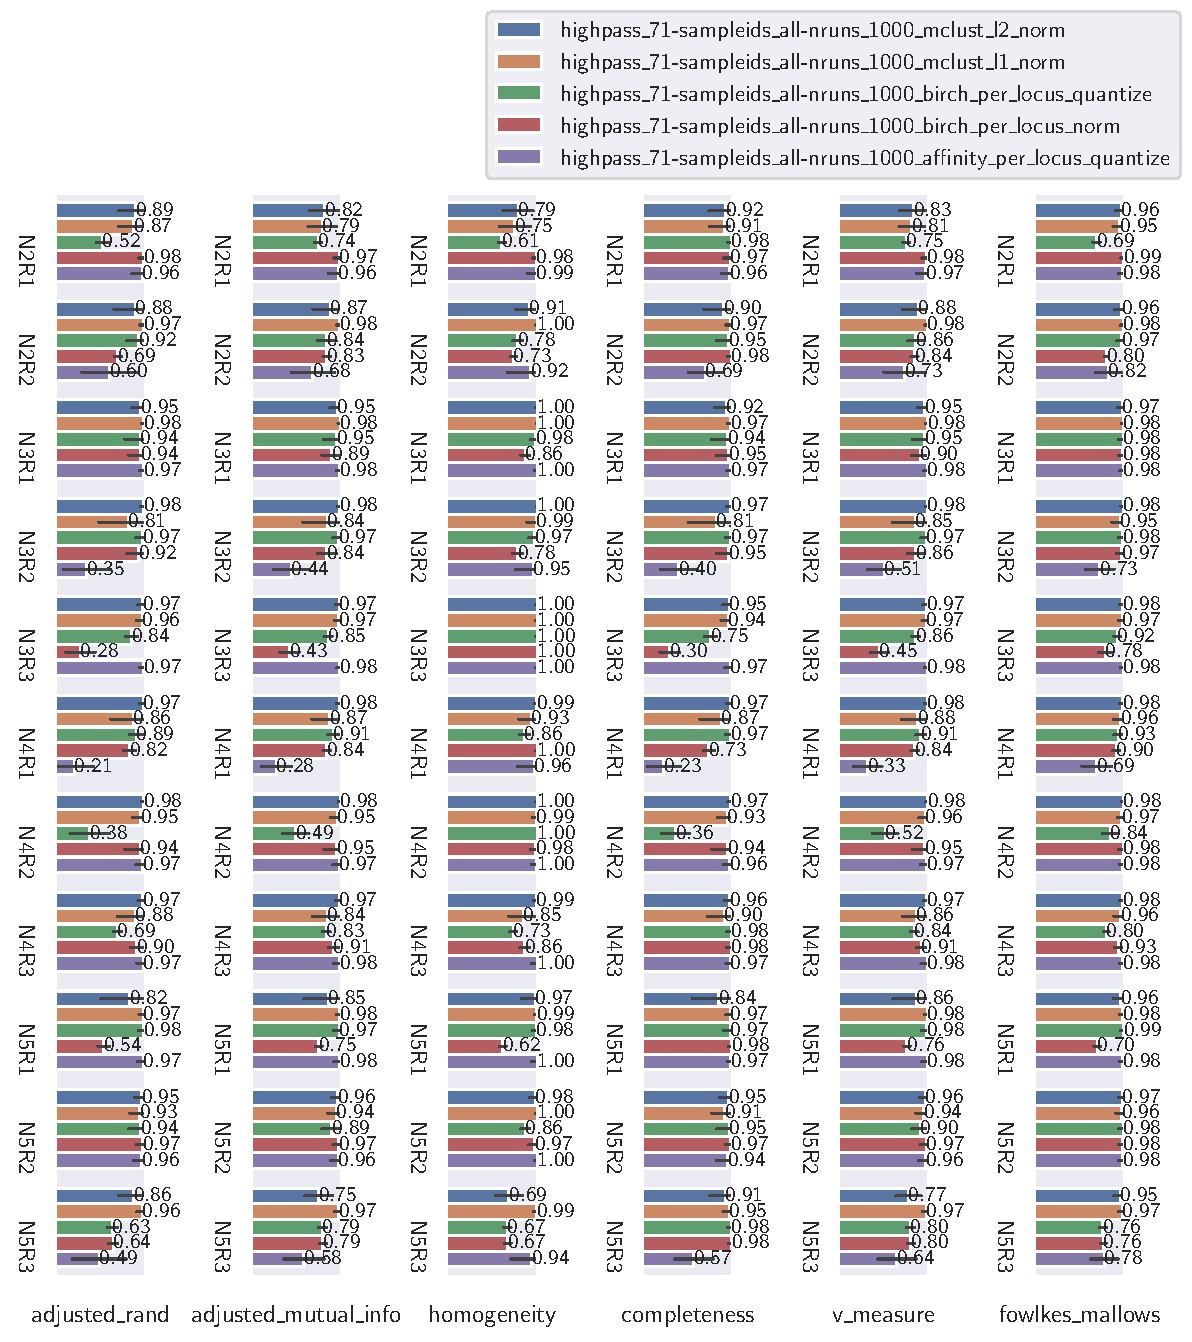
\includegraphics[width=\textwidth]{./figures/clust_comparison/highpass_71-sampleids_all-nruns_1000_top_5_clusterers_by_metrics.pdf}
\caption{Top 5 clusterers clustering performance metrics using 1000 trials sampled from all EPGs with high-pass filtering}
\label{fig:highpass_71-sampleids_all-nruns_1000_top_5_clusterers_by_metrics}
\end{figure}

\begin{table}[H]
\centering
\maxsizebox{\textwidth}{0.65\textwidth}{
\begin{tabular}{lrr}
\toprule
{} &   mean &    std \\
clusterer                                          &        &        \\
\midrule
mclust\_l1\_norm                                     & 55.81\% & 16.52\% \\
mclust\_l2\_norm                                     & 55.11\% & 21.59\% \\
affinity\_per\_locus\_quantize                        & 43.65\% & 33.43\% \\
hdbscan\_cosine\_epsilon\_0.0\_eom\_per\_locus\_norm      & 43.43\% & 34.65\% \\
hdbscan\_euclidean\_epsilon\_0.0\_eom\_per\_locus\_norm   & 43.29\% & 34.62\% \\
hdbscan\_euclidean\_epsilon\_0.5\_eom\_per\_locus\_norm   & 43.29\% & 34.62\% \\
hdbscan\_euclidean\_epsilon\_1.0\_eom\_per\_locus\_norm   & 43.29\% & 34.62\% \\
affinity\_l2\_norm                                   & 42.88\% & 33.43\% \\
affinity\_per\_locus\_norm                            & 42.69\% & 33.26\% \\
hdbscan\_euclidean\_epsilon\_0.0\_eom\_per\_locus\_qua... & 42.66\% & 34.18\% \\
hdbscan\_euclidean\_epsilon\_0.0\_eom\_l2\_norm          & 42.08\% & 33.79\% \\
hdbscan\_euclidean\_epsilon\_0.5\_eom\_l2\_norm          & 42.08\% & 33.79\% \\
hdbscan\_cosine\_epsilon\_0.0\_eom                     & 41.60\% & 33.41\% \\
hdbscan\_euclidean\_epsilon\_0.5\_leaf\_l2\_norm         & 40.84\% & 32.82\% \\
affinity\_l1\_norm                                   & 38.79\% & 30.17\% \\
hdbscan\_euclidean\_epsilon\_0.0\_eom\_l1\_norm          & 32.90\% & 27.37\% \\
hdbscan\_cosine\_epsilon\_0.0\_eom\_per\_locus\_quantize  & 31.86\% & 25.94\% \\
hdbscan\_cosine\_epsilon\_0.5\_eom\_per\_locus\_norm      & 29.40\% & 27.16\% \\
hdbscan\_cosine\_epsilon\_0.5\_leaf\_per\_locus\_norm     & 29.40\% & 27.16\% \\
birch\_l2\_norm                                      & 25.36\% & 29.54\% \\
birch\_per\_locus\_norm                               & 23.08\% & 38.11\% \\
birch\_per\_locus\_quantize                           & 23.01\% & 38.01\% \\
optics\_per\_locus\_quantize                          & 18.10\% & 16.29\% \\
meanshift\_per\_locus\_norm                           & 17.31\% & 16.69\% \\
hdbscan\_cosine\_epsilon\_0.5\_eom                     & 17.25\% & 25.24\% \\
\bottomrule
\end{tabular}


}
\caption{Top 25 clusterers by arithmetic mean of percentages of perfect clustering, using admixtures sampled from all EPG data with highpass filter}
\label{table:top_25_not_ensemble_clusterers_by_binomial_confidence_highpass_71-sampleids_all-nruns_1000}
\end{table}

\begin{table}[H]
\centering
\maxsizebox{\textwidth}{0.65\textwidth}{
\begin{tabular}{llrrrrrrrrrr}
\toprule
     & {} & \multicolumn{5}{l}{homogeneity} & \multicolumn{5}{l}{completeness} \\
     & clusterer &           1 &      2 &      3 &      4 &      5 &            1 &      2 &      3 &      4 &      5 \\
\midrule
N2R1 & ci\_upp &      23.94\% & 27.16\% & 97.39\% & 98.62\% &  4.02\% &       77.87\% & 83.97\% & 82.93\% & 86.33\% & 32.09\% \\
     & success &      21.30\% & 24.40\% & 96.40\% & 97.90\% &  2.80\% &       75.30\% & 81.70\% & 80.60\% & 84.20\% & 29.20\% \\
     & ci\_low &      18.87\% & 21.84\% & 95.06\% & 96.81\% &  1.94\% &       72.53\% & 79.18\% & 78.03\% & 81.81\% & 26.47\% \\
N2R2 & ci\_upp &      94.06\% & 64.27\% & 89.31\% & 98.78\% &  0.38\% &       65.06\% & 83.31\% &  9.85\% & 79.02\% & 31.07\% \\
     & success &      92.60\% & 61.30\% & 87.40\% & 98.10\% &  0.00\% &       62.10\% & 81.00\% &  8.00\% & 76.50\% & 28.20\% \\
     & ci\_low &      90.81\% & 58.24\% & 85.20\% & 97.05\% &  0.00\% &       59.05\% & 78.45\% &  6.47\% & 73.77\% & 25.50\% \\
N3R1 & ci\_upp &      90.88\% & 99.01\% & 94.96\% & 98.46\% & 50.60\% &       59.05\% & 76.24\% & 65.64\% & 72.57\% & 70.43\% \\
     & success &      89.10\% & 98.40\% & 93.60\% & 97.70\% & 47.50\% &       56.00\% & 73.60\% & 62.70\% & 69.80\% & 67.60\% \\
     & ci\_low &      87.02\% & 97.42\% & 91.91\% & 96.57\% & 44.42\% &       52.91\% & 70.78\% & 59.66\% & 66.88\% & 64.64\% \\
N3R2 & ci\_upp &      98.94\% & 94.87\% & 94.78\% &  0.38\% & 98.94\% &       75.85\% & 68.09\% &  6.08\% & 32.20\% & 65.55\% \\
     & success &      98.30\% & 93.50\% & 93.40\% &  0.00\% & 98.30\% &       73.20\% & 65.20\% &  4.60\% & 29.30\% & 62.60\% \\
     & ci\_low &      97.29\% & 91.80\% & 91.69\% &  0.00\% & 97.29\% &       70.37\% & 62.19\% &  3.47\% & 26.56\% & 59.56\% \\
N3R3 & ci\_upp &      96.71\% & 97.05\% & 96.27\% &  5.06\% &  0.38\% &       66.33\% & 71.21\% & 72.76\% & 29.01\% & 35.97\% \\
     & success &      95.60\% & 96.00\% & 95.10\% &  3.70\% &  0.00\% &       63.40\% & 68.40\% & 70.00\% & 26.20\% & 33.00\% \\
     & ci\_low &      94.14\% & 94.60\% & 93.58\% &  2.70\% &  0.00\% &       60.37\% & 65.45\% & 67.09\% & 23.57\% & 30.16\% \\
N4R1 & ci\_upp &      74.60\% & 82.74\% & 96.96\% & 98.14\% & 98.62\% &       78.54\% & 62.11\% &  4.25\% & 69.65\% & 72.37\% \\
     & success &      71.90\% & 80.40\% & 95.90\% & 97.30\% & 97.90\% &       76.00\% & 59.10\% &  3.00\% & 66.80\% & 69.60\% \\
     & ci\_low &      69.03\% & 77.83\% & 94.49\% & 96.10\% & 96.81\% &       73.26\% & 56.02\% &  2.11\% & 63.82\% & 66.68\% \\
N4R2 & ci\_upp &      93.53\% & 89.31\% & 98.78\% &  0.38\% &  0.38\% &       74.89\% & 60.63\% & 73.44\% & 26.12\% & 33.22\% \\
     & success &      92.00\% & 87.40\% & 98.10\% &  0.00\% &  0.00\% &       72.20\% & 57.60\% & 70.70\% & 23.40\% & 30.30\% \\
     & ci\_low &      90.15\% & 85.20\% & 97.05\% &  0.00\% &  0.00\% &       69.34\% & 54.51\% & 67.80\% & 20.88\% & 27.53\% \\
N4R3 & ci\_upp &      45.49\% & 87.17\% & 98.70\% &  0.38\% & 97.56\% &       80.65\% & 69.94\% & 66.62\% & 32.40\% & 76.72\% \\
     & success &      42.40\% & 85.10\% & 98.00\% &  0.00\% & 96.60\% &       78.20\% & 67.10\% & 63.70\% & 29.50\% & 74.10\% \\
     & ci\_low &      39.37\% & 82.76\% & 96.93\% &  0.00\% & 95.29\% &       75.54\% & 64.13\% & 60.67\% & 26.76\% & 71.30\% \\
N5R1 & ci\_upp &      85.39\% & 97.89\% & 97.81\% & 97.89\% & 99.16\% &       61.12\% & 79.69\% & 59.15\% & 65.55\% & 78.93\% \\
     & success &      83.20\% & 97.00\% & 96.90\% & 97.00\% & 98.60\% &       58.10\% & 77.20\% & 56.10\% & 62.60\% & 76.40\% \\
     & ci\_low &      80.76\% & 95.75\% & 95.63\% & 95.75\% & 97.66\% &       55.02\% & 74.50\% & 53.01\% & 59.56\% & 73.67\% \\
N5R2 & ci\_upp &      98.62\% & 89.31\% & 99.59\% & 51.90\% & 98.38\% &       71.89\% & 79.41\% & 79.41\% & 71.11\% & 69.65\% \\
     & success &      97.90\% & 87.40\% & 99.20\% & 48.80\% & 97.60\% &       69.10\% & 76.90\% & 76.90\% & 68.30\% & 66.80\% \\
     & ci\_low &      96.81\% & 85.20\% & 98.43\% & 45.71\% & 96.45\% &       66.17\% & 74.19\% & 74.19\% & 65.35\% & 63.82\% \\
N5R3 & ci\_upp &      88.94\% & 11.04\% & 91.98\% & 96.88\% & 99.01\% &       65.84\% & 79.69\% &  8.64\% & 76.43\% & 86.14\% \\
     & success &      87.00\% &  9.10\% & 90.30\% & 95.80\% & 98.40\% &       62.90\% & 77.20\% &  6.90\% & 73.80\% & 84.00\% \\
     & ci\_low &      84.77\% &  7.47\% & 88.31\% & 94.37\% & 97.42\% &       59.86\% & 74.50\% &  5.49\% & 70.99\% & 81.60\% \\
\bottomrule
\end{tabular}


}
\caption{Top 5 clusterers clustering percentages of trials where no error occurs using 1000 trials sampled from all EPGs with high-pass filtering}
\label{table:highpass_71-sampleids_all-nruns_1000_top_5_clusterers_by_binomial_confidence}
\end{table}

%--------------------------------------------------------------------------------------------------------------------------------------------
\section{Experiments Results---Clusterer Ensembles}

\begin{table}
\centering
\begin{tabular}{l}
\toprule
                                    Clusterer Name \\
\midrule
                           affinity\_per\_locus\_norm \\
                       affinity\_per\_locus\_quantize \\
                                     birch\_l2\_norm \\
                              birch\_per\_locus\_norm \\
                          birch\_per\_locus\_quantize \\
     hdbscan\_cosine\_epsilon\_0.0\_eom\_per\_locus\_norm \\
  hdbscan\_euclidean\_epsilon\_0.0\_eom\_per\_locus\_norm \\
hdbscan\_euclidean\_epsilon\_0.0\_eom\_per\_locus\_qua... \\
                                    mclust\_l1\_norm \\
                                    mclust\_l2\_norm \\
                          meanshift\_per\_locus\_norm \\
                      meanshift\_per\_locus\_quantize \\
\bottomrule
\end{tabular}
\caption{Clusterers selected to form cluster ensembles}
\label{table:Clusterers selected to form cluster ensembles}
\end{table}

\subsection{Saliva Samples Only, without High-Pass Filtering}

\begin{figure}[H]
\centering
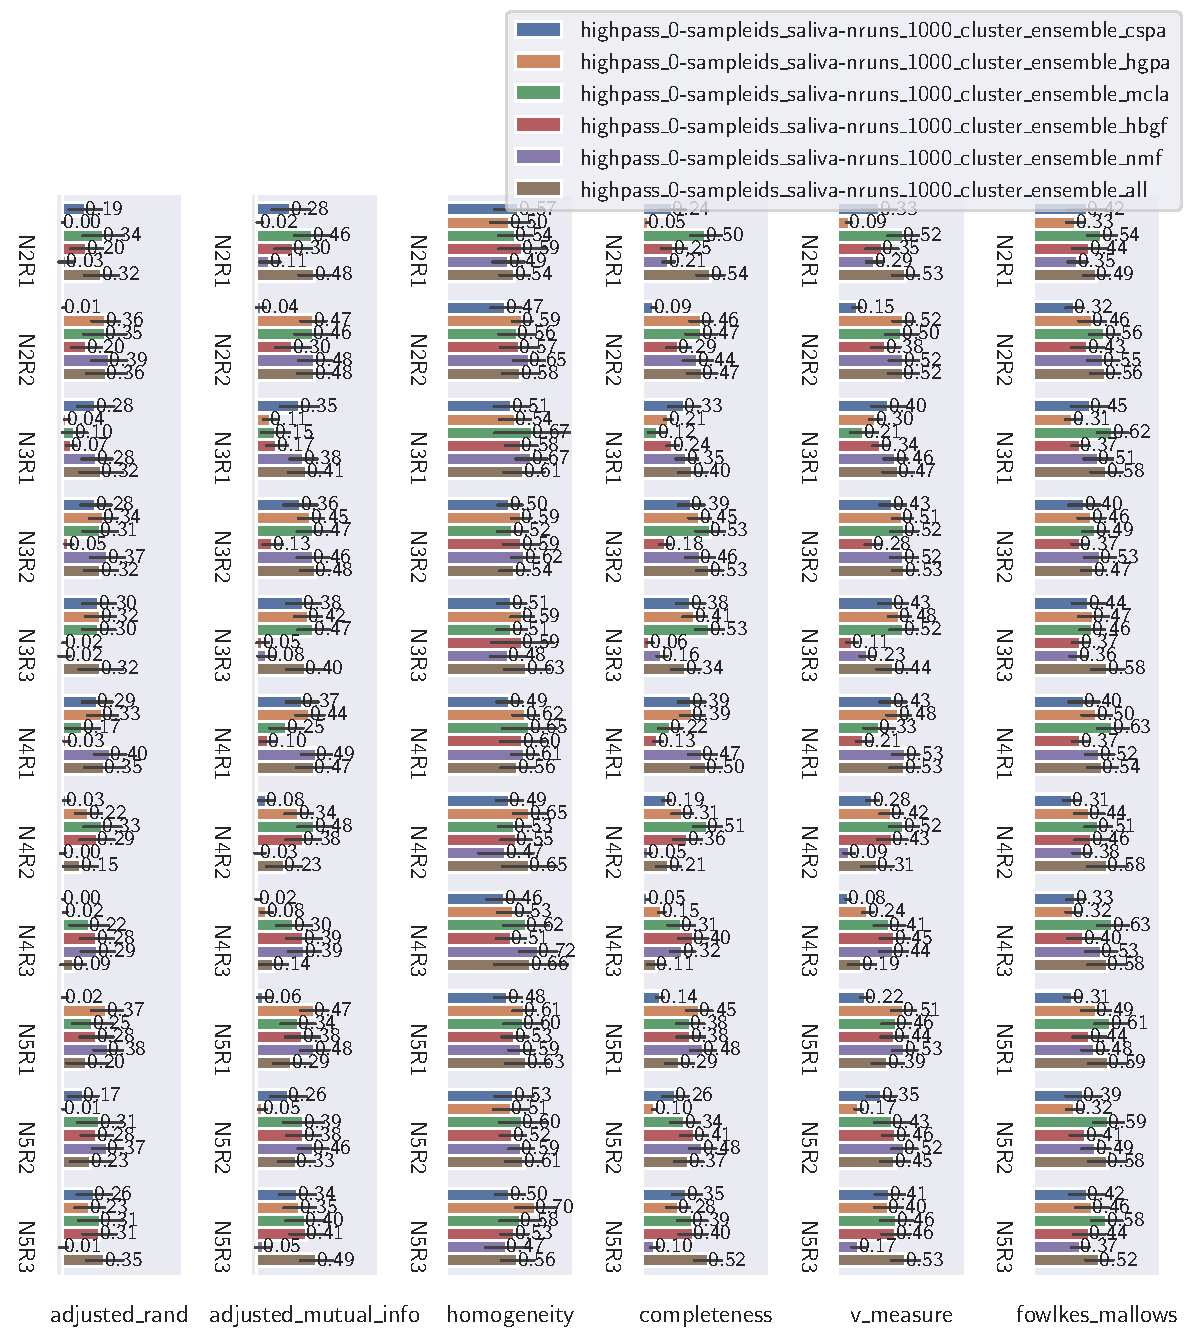
\includegraphics[width=\textwidth]{./figures/clust_comparison/highpass_0-sampleids_saliva-nruns_1000_cluster_ensembles.pdf}
\caption{Cluster ensembles clustering performance metrics using 1000 trials sampled from EPGs from only saliva samples without high-pass filtering}
\label{fig:highpass_0-sampleids_saliva-nruns_1000_cluster_ensembles}
\end{figure}

\begin{table}[H]
\centering
\maxsizebox{\textwidth}{0.65\textwidth}{
\begin{tabular}{llrrrrrrrrrrrr}
\toprule
     & {} & \multicolumn{6}{l}{homogeneity} & \multicolumn{6}{l}{completeness} \\
     & clusterer &           1 &     2 &      3 &      4 &      5 &      6 &            1 &     2 &     3 &     4 &     5 &     6 \\
\midrule
N2R1 & ci\_upp &       2.34\% & 2.46\% &  0.38\% &  2.34\% &  0.38\% &  0.38\% &        0.38\% & 0.38\% & 0.38\% & 0.38\% & 0.38\% & 0.38\% \\
     & success &       1.40\% & 1.50\% &  0.00\% &  1.40\% &  0.00\% &  0.00\% &        0.00\% & 0.00\% & 0.00\% & 0.00\% & 0.00\% & 0.00\% \\
     & ci\_low &       0.84\% & 0.91\% &  0.00\% &  0.84\% &  0.00\% &  0.00\% &        0.00\% & 0.00\% & 0.00\% & 0.00\% & 0.00\% & 0.00\% \\
N2R2 & ci\_upp &       0.38\% & 0.38\% &  0.38\% &  0.56\% &  0.38\% &  0.38\% &        0.38\% & 0.38\% & 0.38\% & 0.38\% & 0.38\% & 0.38\% \\
     & success &       0.00\% & 0.00\% &  0.00\% &  0.10\% &  0.00\% &  0.00\% &        0.00\% & 0.00\% & 0.00\% & 0.00\% & 0.00\% & 0.00\% \\
     & ci\_low &       0.00\% & 0.00\% &  0.00\% &  0.02\% &  0.00\% &  0.00\% &        0.00\% & 0.00\% & 0.00\% & 0.00\% & 0.00\% & 0.00\% \\
N3R1 & ci\_upp &       0.38\% & 0.38\% & 39.63\% &  0.38\% &  1.02\% &  0.73\% &        0.38\% & 0.38\% & 0.38\% & 0.38\% & 0.38\% & 0.38\% \\
     & success &       0.00\% & 0.00\% & 36.60\% &  0.00\% &  0.40\% &  0.20\% &        0.00\% & 0.00\% & 0.00\% & 0.00\% & 0.00\% & 0.00\% \\
     & ci\_low &       0.00\% & 0.00\% & 33.67\% &  0.00\% &  0.16\% &  0.05\% &        0.00\% & 0.00\% & 0.00\% & 0.00\% & 0.00\% & 0.00\% \\
N3R2 & ci\_upp &       0.38\% & 0.38\% &  0.38\% &  0.56\% &  0.38\% &  0.38\% &        0.38\% & 0.38\% & 0.38\% & 0.38\% & 0.38\% & 0.38\% \\
     & success &       0.00\% & 0.00\% &  0.00\% &  0.10\% &  0.00\% &  0.00\% &        0.00\% & 0.00\% & 0.00\% & 0.00\% & 0.00\% & 0.00\% \\
     & ci\_low &       0.00\% & 0.00\% &  0.00\% &  0.02\% &  0.00\% &  0.00\% &        0.00\% & 0.00\% & 0.00\% & 0.00\% & 0.00\% & 0.00\% \\
N3R3 & ci\_upp &       0.38\% & 0.38\% &  0.38\% & 20.29\% &  0.38\% &  2.34\% &        0.38\% & 0.38\% & 0.38\% & 0.38\% & 0.38\% & 0.38\% \\
     & success &       0.00\% & 0.00\% &  0.00\% & 17.80\% &  0.00\% &  1.40\% &        0.00\% & 0.00\% & 0.00\% & 0.00\% & 0.00\% & 0.00\% \\
     & ci\_low &       0.00\% & 0.00\% &  0.00\% & 15.55\% &  0.00\% &  0.84\% &        0.00\% & 0.00\% & 0.00\% & 0.00\% & 0.00\% & 0.00\% \\
N4R1 & ci\_upp &       0.38\% & 0.38\% & 14.69\% &  3.66\% &  0.38\% &  0.38\% &        0.38\% & 0.38\% & 0.38\% & 0.38\% & 0.38\% & 0.38\% \\
     & success &       0.00\% & 0.00\% & 12.50\% &  2.50\% &  0.00\% &  0.00\% &        0.00\% & 0.00\% & 0.00\% & 0.00\% & 0.00\% & 0.00\% \\
     & ci\_low &       0.00\% & 0.00\% & 10.59\% &  1.70\% &  0.00\% &  0.00\% &        0.00\% & 0.00\% & 0.00\% & 0.00\% & 0.00\% & 0.00\% \\
N4R2 & ci\_upp &       0.38\% & 0.38\% &  0.38\% &  0.38\% & 11.48\% & 13.95\% &        0.38\% & 0.38\% & 0.38\% & 0.38\% & 0.38\% & 0.38\% \\
     & success &       0.00\% & 0.00\% &  0.00\% &  0.00\% &  9.50\% & 11.80\% &        0.00\% & 0.00\% & 0.00\% & 0.00\% & 0.00\% & 0.00\% \\
     & ci\_low &       0.00\% & 0.00\% &  0.00\% &  0.00\% &  7.83\% &  9.95\% &        0.00\% & 0.00\% & 0.00\% & 0.00\% & 0.00\% & 0.00\% \\
N4R3 & ci\_upp &       0.73\% & 0.38\% &  4.13\% &  0.38\% &  4.25\% & 37.81\% &        0.38\% & 0.38\% & 0.38\% & 0.38\% & 0.38\% & 0.38\% \\
     & success &       0.20\% & 0.00\% &  2.90\% &  0.00\% &  3.00\% & 34.80\% &        0.00\% & 0.00\% & 0.00\% & 0.00\% & 0.00\% & 0.00\% \\
     & ci\_low &       0.05\% & 0.00\% &  2.03\% &  0.00\% &  2.11\% & 31.91\% &        0.00\% & 0.00\% & 0.00\% & 0.00\% & 0.00\% & 0.00\% \\
N5R1 & ci\_upp &       0.38\% & 0.38\% &  1.02\% &  0.38\% &  0.38\% &  3.90\% &        0.38\% & 0.38\% & 0.38\% & 0.38\% & 0.38\% & 0.38\% \\
     & success &       0.00\% & 0.00\% &  0.40\% &  0.00\% &  0.00\% &  2.70\% &        0.00\% & 0.00\% & 0.00\% & 0.00\% & 0.00\% & 0.00\% \\
     & ci\_low &       0.00\% & 0.00\% &  0.16\% &  0.00\% &  0.00\% &  1.86\% &        0.00\% & 0.00\% & 0.00\% & 0.00\% & 0.00\% & 0.00\% \\
N5R2 & ci\_upp &       0.38\% & 0.73\% &  1.83\% &  0.38\% &  0.38\% &  1.02\% &        0.38\% & 0.38\% & 0.38\% & 0.38\% & 0.38\% & 0.38\% \\
     & success &       0.00\% & 0.20\% &  1.00\% &  0.00\% &  0.00\% &  0.40\% &        0.00\% & 0.00\% & 0.00\% & 0.00\% & 0.00\% & 0.00\% \\
     & ci\_low &       0.00\% & 0.05\% &  0.54\% &  0.00\% &  0.00\% &  0.16\% &        0.00\% & 0.00\% & 0.00\% & 0.00\% & 0.00\% & 0.00\% \\
N5R3 & ci\_upp &       0.38\% & 9.52\% &  0.56\% &  0.38\% &  0.56\% &  0.38\% &        0.38\% & 0.38\% & 0.38\% & 0.38\% & 0.38\% & 0.38\% \\
     & success &       0.00\% & 7.70\% &  0.10\% &  0.00\% &  0.10\% &  0.00\% &        0.00\% & 0.00\% & 0.00\% & 0.00\% & 0.00\% & 0.00\% \\
     & ci\_low &       0.00\% & 6.20\% &  0.02\% &  0.00\% &  0.02\% &  0.00\% &        0.00\% & 0.00\% & 0.00\% & 0.00\% & 0.00\% & 0.00\% \\
\bottomrule
\end{tabular}


}
\caption{Cluster ensembles clustering percentages of trials where no error occurs using 1000 trials sampled from EPGs from only saliva samples without high-pass filtering}
\label{table:highpass_0-sampleids_saliva-nruns_1000_cluster_ensembles}
\end{table}

\subsection{Saliva Samples Only, with High-Pass Filtering}

\begin{figure}[H]
\centering
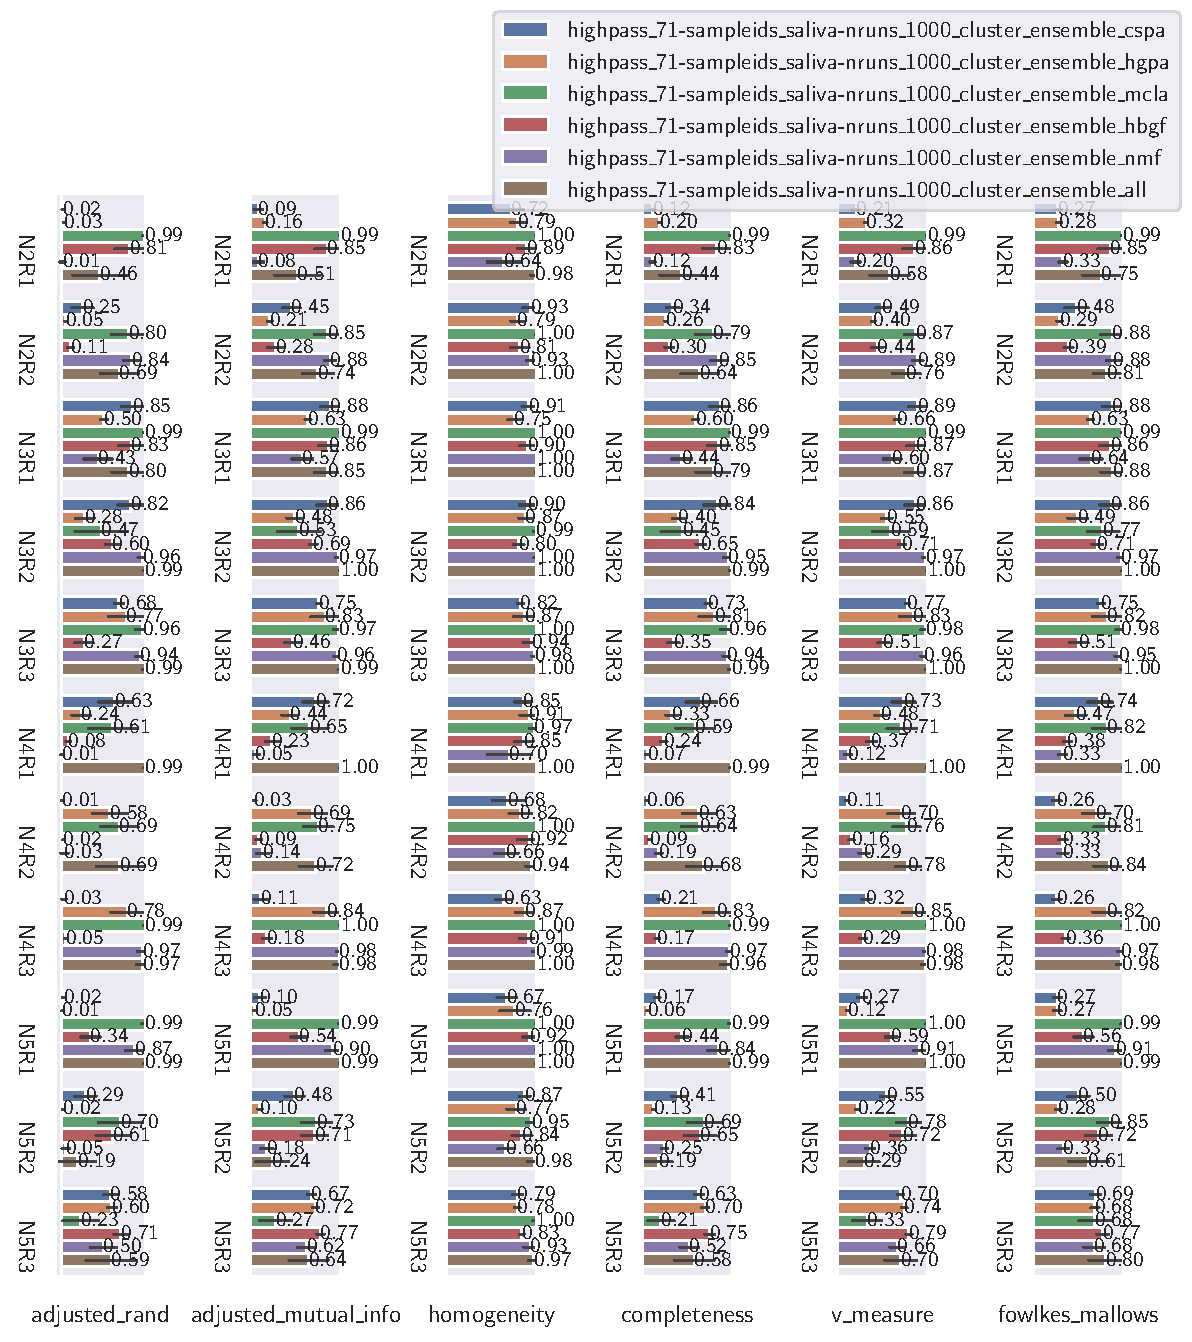
\includegraphics[width=\textwidth]{./figures/clust_comparison/highpass_71-sampleids_saliva-nruns_1000_cluster_ensembles.pdf}
\caption{Cluster ensembles clustering performance metrics using 1000 trials sampled from EPGs from only saliva samples with high-pass filtering}
\label{fig:highpass_71-sampleids_saliva-nruns_1000_cluster_ensembles}
\end{figure}

\begin{table}[H]
\centering
\maxsizebox{\textwidth}{0.65\textwidth}{
\begin{tabular}{llrrrrrrrrrrrr}
\toprule
     & {} & \multicolumn{6}{l}{homogeneity} & \multicolumn{6}{l}{completeness} \\
     & clusterer &           1 &      2 &       3 &      4 &       5 &       6 &            1 &      2 &      3 &      4 &      5 &      6 \\
\midrule
N2R1 & ci\_upp &       7.09\% &  0.38\% &  98.30\% & 48.80\% &   3.31\% &  91.16\% &        0.38\% &  0.38\% & 90.24\% & 48.80\% &  0.38\% &  5.63\% \\
     & success &       5.50\% &  0.00\% &  97.50\% & 45.70\% &   2.20\% &  89.40\% &        0.00\% &  0.00\% & 88.40\% & 45.70\% &  0.00\% &  4.20\% \\
     & ci\_low &       4.25\% &  0.00\% &  96.34\% & 42.63\% &   1.46\% &  87.34\% &        0.00\% &  0.00\% & 86.27\% & 42.63\% &  0.00\% &  3.12\% \\
N2R2 & ci\_upp &      60.83\% &  0.38\% &  98.78\% &  5.29\% &  39.94\% &  99.98\% &        0.38\% &  0.38\% & 41.66\% &  0.38\% & 16.82\% & 18.30\% \\
     & success &      57.80\% &  0.00\% &  98.10\% &  3.90\% &  36.90\% &  99.90\% &        0.00\% &  0.00\% & 38.60\% &  0.00\% & 14.50\% & 15.90\% \\
     & ci\_low &      54.71\% &  0.00\% &  97.05\% &  2.87\% &  33.96\% &  99.44\% &        0.00\% &  0.00\% & 35.63\% &  0.00\% & 12.45\% & 13.76\% \\
N3R1 & ci\_upp &      46.39\% &  0.56\% &  99.66\% & 35.77\% & 100.00\% &  98.70\% &       46.39\% &  0.38\% & 84.07\% & 35.77\% &  0.73\% & 41.66\% \\
     & success &      43.30\% &  0.10\% &  99.30\% & 32.80\% & 100.00\% &  98.00\% &       43.30\% &  0.00\% & 81.80\% & 32.80\% &  0.20\% & 38.60\% \\
     & ci\_low &      40.26\% &  0.02\% &  98.56\% & 29.96\% &  99.62\% &  96.93\% &       40.26\% &  0.00\% & 79.29\% & 29.96\% &  0.05\% & 35.63\% \\
N3R2 & ci\_upp &      48.80\% &  5.51\% &  94.96\% &  3.78\% &  99.01\% & 100.00\% &       48.80\% &  0.38\% &  5.63\% &  0.73\% & 52.10\% & 92.80\% \\
     & success &      45.70\% &  4.10\% &  93.60\% &  2.60\% &  98.40\% & 100.00\% &       45.70\% &  0.00\% &  4.20\% &  0.20\% & 49.00\% & 91.20\% \\
     & ci\_low &      42.63\% &  3.04\% &  91.91\% &  1.78\% &  97.42\% &  99.62\% &       42.63\% &  0.00\% &  3.12\% &  0.05\% & 45.91\% & 89.28\% \\
N3R3 & ci\_upp &       0.38\% & 48.80\% & 100.00\% & 67.01\% &  74.50\% &  99.01\% &        0.73\% & 48.80\% & 83.50\% &  0.38\% & 39.43\% & 96.62\% \\
     & success &       0.00\% & 45.70\% & 100.00\% & 64.10\% &  71.80\% &  98.40\% &        0.20\% & 45.70\% & 81.20\% &  0.00\% & 36.40\% & 95.50\% \\
     & ci\_low &       0.00\% & 42.63\% &  99.62\% & 61.08\% &  68.93\% &  97.42\% &        0.05\% & 42.63\% & 78.66\% &  0.00\% & 33.48\% & 94.03\% \\
N4R1 & ci\_upp &      24.26\% & 50.30\% &  76.05\% & 18.09\% &  38.62\% &  99.98\% &       21.13\% &  0.38\% &  4.37\% &  0.38\% &  0.38\% & 85.58\% \\
     & success &      21.60\% & 47.20\% &  73.40\% & 15.70\% &  35.60\% &  99.90\% &       18.60\% &  0.00\% &  3.10\% &  0.00\% &  0.00\% & 83.40\% \\
     & ci\_low &      19.16\% & 44.12\% &  70.58\% & 13.58\% &  32.69\% &  99.44\% &       16.31\% &  0.00\% &  2.19\% &  0.00\% &  0.00\% & 80.97\% \\
N4R2 & ci\_upp &      18.61\% & 30.97\% &  99.84\% & 73.63\% &   0.38\% &  46.39\% &        0.38\% & 21.13\% & 18.19\% &  0.38\% &  0.38\% &  4.37\% \\
     & success &      16.20\% & 28.10\% &  99.60\% & 70.90\% &   0.00\% &  43.30\% &        0.00\% & 18.60\% & 15.80\% &  0.00\% &  0.00\% &  3.10\% \\
     & ci\_low &      14.05\% & 25.40\% &  98.98\% & 68.01\% &   0.00\% &  40.26\% &        0.00\% & 16.31\% & 13.67\% &  0.00\% &  0.00\% &  2.19\% \\
N4R3 & ci\_upp &       0.38\% & 46.39\% &  99.90\% & 44.68\% &  95.66\% & 100.00\% &        0.38\% & 46.39\% & 92.35\% &  0.38\% & 47.50\% & 83.88\% \\
     & success &       0.00\% & 43.30\% &  99.70\% & 41.60\% &  94.40\% & 100.00\% &        0.00\% & 43.30\% & 90.70\% &  0.00\% & 44.40\% & 81.60\% \\
     & ci\_low &       0.00\% & 40.26\% &  99.12\% & 38.58\% &  92.80\% &  99.62\% &        0.00\% & 40.26\% & 88.74\% &  0.00\% & 41.35\% & 79.08\% \\
N5R1 & ci\_upp &       0.73\% & 31.38\% &  99.01\% & 36.69\% &  99.98\% &  98.46\% &        0.38\% &  0.38\% & 96.62\% &  0.38\% & 26.33\% & 90.79\% \\
     & success &       0.20\% & 28.50\% &  98.40\% & 33.70\% &  99.90\% &  97.70\% &        0.00\% &  0.00\% & 95.50\% &  0.00\% & 23.60\% & 89.00\% \\
     & ci\_low &       0.05\% & 25.79\% &  97.42\% & 30.84\% &  99.44\% &  96.57\% &        0.00\% &  0.00\% & 94.03\% &  0.00\% & 21.07\% & 86.91\% \\
N5R2 & ci\_upp &       2.58\% &  4.83\% &  47.19\% & 26.33\% &   0.38\% &  94.06\% &        0.38\% &  0.38\% &  4.37\% & 21.13\% &  0.38\% &  1.17\% \\
     & success &       1.60\% &  3.50\% &  44.10\% & 23.60\% &   0.00\% &  92.60\% &        0.00\% &  0.00\% &  3.10\% & 18.60\% &  0.00\% &  0.50\% \\
     & ci\_low &       0.99\% &  2.53\% &  41.05\% & 21.07\% &   0.00\% &  90.81\% &        0.00\% &  0.00\% &  2.19\% & 16.31\% &  0.00\% &  0.21\% \\
N5R3 & ci\_upp &       0.38\% &  0.38\% &  99.31\% &  0.38\% &  48.50\% &  73.15\% &        0.73\% &  0.73\% &  1.30\% &  0.73\% &  0.88\% &  4.13\% \\
     & success &       0.00\% &  0.00\% &  98.80\% &  0.00\% &  45.40\% &  70.40\% &        0.20\% &  0.20\% &  0.60\% &  0.20\% &  0.30\% &  2.90\% \\
     & ci\_low &       0.00\% &  0.00\% &  97.91\% &  0.00\% &  42.34\% &  67.50\% &        0.05\% &  0.05\% &  0.28\% &  0.05\% &  0.10\% &  2.03\% \\
\bottomrule
\end{tabular}


}
\caption{Cluster ensembles clustering percentages of trials where no error occurs using 1000 trials sampled from EPGs from only saliva samples with high-pass filtering}
\label{table:highpass_71-sampleids_saliva-nruns_1000_cluster_ensembles}
\end{table}

\subsection{Blood Samples Only, without High-Pass Filtering}

\begin{figure}[H]
\centering
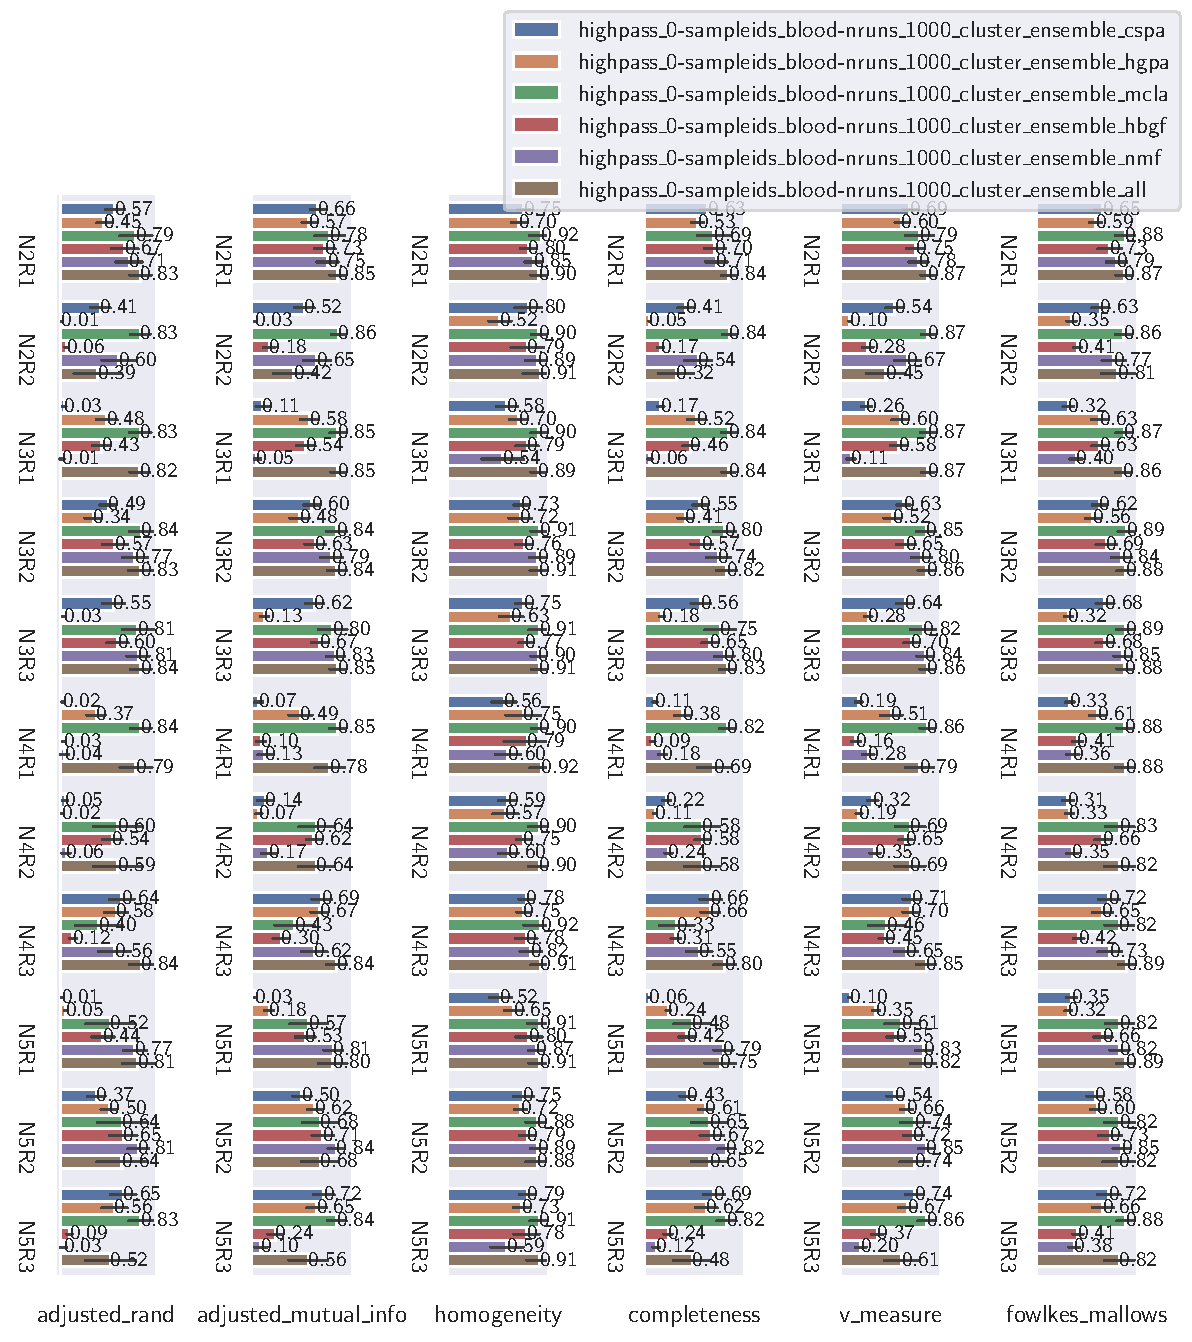
\includegraphics[width=\textwidth]{./figures/clust_comparison/highpass_0-sampleids_blood-nruns_1000_cluster_ensembles.pdf}
\caption{Cluster ensembles clustering performance metrics using 1000 trials sampled from EPGs from only blood samples without high-pass filtering}
\label{fig:highpass_0-sampleids_blood-nruns_1000_cluster_ensembles}
\end{figure}

\begin{table}[H]
\centering
\maxsizebox{\textwidth}{0.65\textwidth}{
\begin{tabular}{llrrrrrrrrrrrr}
\toprule
     & {} & \multicolumn{6}{l}{homogeneity} & \multicolumn{6}{l}{completeness} \\
     & clusterer &           1 &      2 &      3 &      4 &      5 &      6 &            1 &     2 &      3 &     4 &     5 &      6 \\
\midrule
N2R1 & ci\_upp &       0.38\% &  0.38\% & 51.20\% &  0.38\% &  4.60\% &  4.60\% &        0.38\% & 0.38\% &  7.31\% & 0.38\% & 1.02\% &  1.83\% \\
     & success &       0.00\% &  0.00\% & 48.10\% &  0.00\% &  3.30\% &  3.30\% &        0.00\% & 0.00\% &  5.70\% & 0.00\% & 0.40\% &  1.00\% \\
     & ci\_low &       0.00\% &  0.00\% & 45.02\% &  0.00\% &  2.36\% &  2.36\% &        0.00\% & 0.00\% &  4.43\% & 0.00\% & 0.16\% &  0.54\% \\
N2R2 & ci\_upp &      19.98\% &  0.73\% &  1.57\% & 21.44\% & 41.35\% & 78.74\% &        0.38\% & 0.38\% &  0.56\% & 0.38\% & 0.73\% &  1.44\% \\
     & success &      17.50\% &  0.20\% &  0.80\% & 18.90\% & 38.30\% & 76.20\% &        0.00\% & 0.00\% &  0.10\% & 0.00\% & 0.20\% &  0.70\% \\
     & ci\_low &      15.27\% &  0.05\% &  0.41\% & 16.59\% & 35.34\% & 73.46\% &        0.00\% & 0.00\% &  0.02\% & 0.00\% & 0.05\% &  0.34\% \\
N3R1 & ci\_upp &       0.38\% &  4.25\% &  4.60\% &  3.31\% & 12.88\% &  1.70\% &        0.38\% & 2.34\% &  1.83\% & 0.38\% & 0.38\% &  0.56\% \\
     & success &       0.00\% &  3.00\% &  3.30\% &  2.20\% & 10.80\% &  0.90\% &        0.00\% & 1.40\% &  1.00\% & 0.00\% & 0.00\% &  0.10\% \\
     & ci\_low &       0.00\% &  2.11\% &  2.36\% &  1.46\% &  9.02\% &  0.47\% &        0.00\% & 0.84\% &  0.54\% & 0.00\% & 0.00\% &  0.02\% \\
N3R2 & ci\_upp &       0.38\% &  0.38\% & 17.14\% &  2.46\% & 13.52\% & 14.27\% &        0.38\% & 0.38\% &  5.29\% & 2.09\% & 2.95\% &  5.40\% \\
     & success &       0.00\% &  0.00\% & 14.80\% &  1.50\% & 11.40\% & 12.10\% &        0.00\% & 0.00\% &  3.90\% & 1.20\% & 1.90\% &  4.00\% \\
     & ci\_low &       0.00\% &  0.00\% & 12.73\% &  0.91\% &  9.58\% & 10.22\% &        0.00\% & 0.00\% &  2.87\% & 0.69\% & 1.22\% &  2.95\% \\
N3R3 & ci\_upp &       2.71\% &  0.56\% & 38.21\% &  0.38\% &  4.25\% &  5.40\% &        2.09\% & 0.38\% & 13.20\% & 0.38\% & 1.83\% &  1.83\% \\
     & success &       1.70\% &  0.10\% & 35.20\% &  0.00\% &  3.00\% &  4.00\% &        1.20\% & 0.00\% & 11.10\% & 0.00\% & 1.00\% &  1.00\% \\
     & ci\_low &       1.06\% &  0.02\% & 32.30\% &  0.00\% &  2.11\% &  2.95\% &        0.69\% & 0.00\% &  9.30\% & 0.00\% & 0.54\% &  0.54\% \\
N4R1 & ci\_upp &       0.38\% & 26.95\% &  5.51\% & 49.40\% &  0.38\% & 51.20\% &        0.38\% & 0.38\% &  1.96\% & 0.38\% & 0.38\% &  7.31\% \\
     & success &       0.00\% & 24.20\% &  4.10\% & 46.30\% &  0.00\% & 48.10\% &        0.00\% & 0.00\% &  1.10\% & 0.00\% & 0.00\% &  5.70\% \\
     & ci\_low &       0.00\% & 21.65\% &  3.04\% & 43.23\% &  0.00\% & 45.02\% &        0.00\% & 0.00\% &  0.62\% & 0.00\% & 0.00\% &  4.43\% \\
N4R2 & ci\_upp &       0.38\% &  0.38\% & 41.15\% &  0.38\% &  0.38\% & 40.85\% &        0.38\% & 0.38\% &  2.58\% & 0.38\% & 0.38\% &  2.58\% \\
     & success &       0.00\% &  0.00\% & 38.10\% &  0.00\% &  0.00\% & 37.80\% &        0.00\% & 0.00\% &  1.60\% & 0.00\% & 0.00\% &  1.60\% \\
     & ci\_low &       0.00\% &  0.00\% & 35.14\% &  0.00\% &  0.00\% & 34.85\% &        0.00\% & 0.00\% &  0.99\% & 0.00\% & 0.00\% &  0.99\% \\
N4R3 & ci\_upp &       2.21\% &  1.17\% & 79.98\% &  2.58\% &  8.20\% & 17.14\% &        2.21\% & 1.17\% &  1.44\% & 0.38\% & 1.44\% &  5.29\% \\
     & success &       1.30\% &  0.50\% & 77.50\% &  1.60\% &  6.50\% & 14.80\% &        1.30\% & 0.50\% &  0.70\% & 0.00\% & 0.70\% &  3.90\% \\
     & ci\_low &       0.76\% &  0.21\% & 74.81\% &  0.99\% &  5.13\% & 12.73\% &        0.76\% & 0.21\% &  0.34\% & 0.00\% & 0.34\% &  2.87\% \\
N5R1 & ci\_upp &       0.38\% &  0.38\% & 60.33\% & 19.56\% &  2.21\% & 38.21\% &        0.38\% & 0.38\% &  2.58\% & 0.38\% & 1.44\% & 13.20\% \\
     & success &       0.00\% &  0.00\% & 57.30\% & 17.10\% &  1.30\% & 35.20\% &        0.00\% & 0.00\% &  1.60\% & 0.00\% & 0.70\% & 11.10\% \\
     & ci\_low &       0.00\% &  0.00\% & 54.21\% & 14.89\% &  0.76\% & 32.30\% &        0.00\% & 0.00\% &  0.99\% & 0.00\% & 0.34\% &  9.30\% \\
N5R2 & ci\_upp &       0.38\% &  0.38\% & 28.19\% &  1.96\% &  1.17\% & 27.98\% &        0.38\% & 0.38\% &  3.55\% & 1.96\% & 0.56\% &  3.55\% \\
     & success &       0.00\% &  0.00\% & 25.40\% &  1.10\% &  0.50\% & 25.20\% &        0.00\% & 0.00\% &  2.40\% & 1.10\% & 0.10\% &  2.40\% \\
     & ci\_low &       0.00\% &  0.00\% & 22.80\% &  0.62\% &  0.21\% & 22.61\% &        0.00\% & 0.00\% &  1.62\% & 0.62\% & 0.02\% &  1.62\% \\
N5R3 & ci\_upp &       0.73\% &  2.95\% & 14.27\% &  8.86\% &  1.83\% & 60.04\% &        0.73\% & 2.95\% &  5.40\% & 0.38\% & 0.38\% &  2.58\% \\
     & success &       0.20\% &  1.90\% & 12.10\% &  7.10\% &  1.00\% & 57.00\% &        0.20\% & 1.90\% &  4.00\% & 0.00\% & 0.00\% &  1.60\% \\
     & ci\_low &       0.05\% &  1.22\% & 10.22\% &  5.67\% &  0.54\% & 53.91\% &        0.05\% & 1.22\% &  2.95\% & 0.00\% & 0.00\% &  0.99\% \\
\bottomrule
\end{tabular}


}
\caption{Cluster ensembles clustering percentages of trials where no error occurs using 1000 trials sampled from EPGs from only blood samples without high-pass filtering}
\label{table:highpass_0-sampleids_blood-nruns_1000_cluster_ensembles}
\end{table}

\subsection{Blood Samples Only, with High-Pass Filtering}

\begin{figure}[H]
\centering
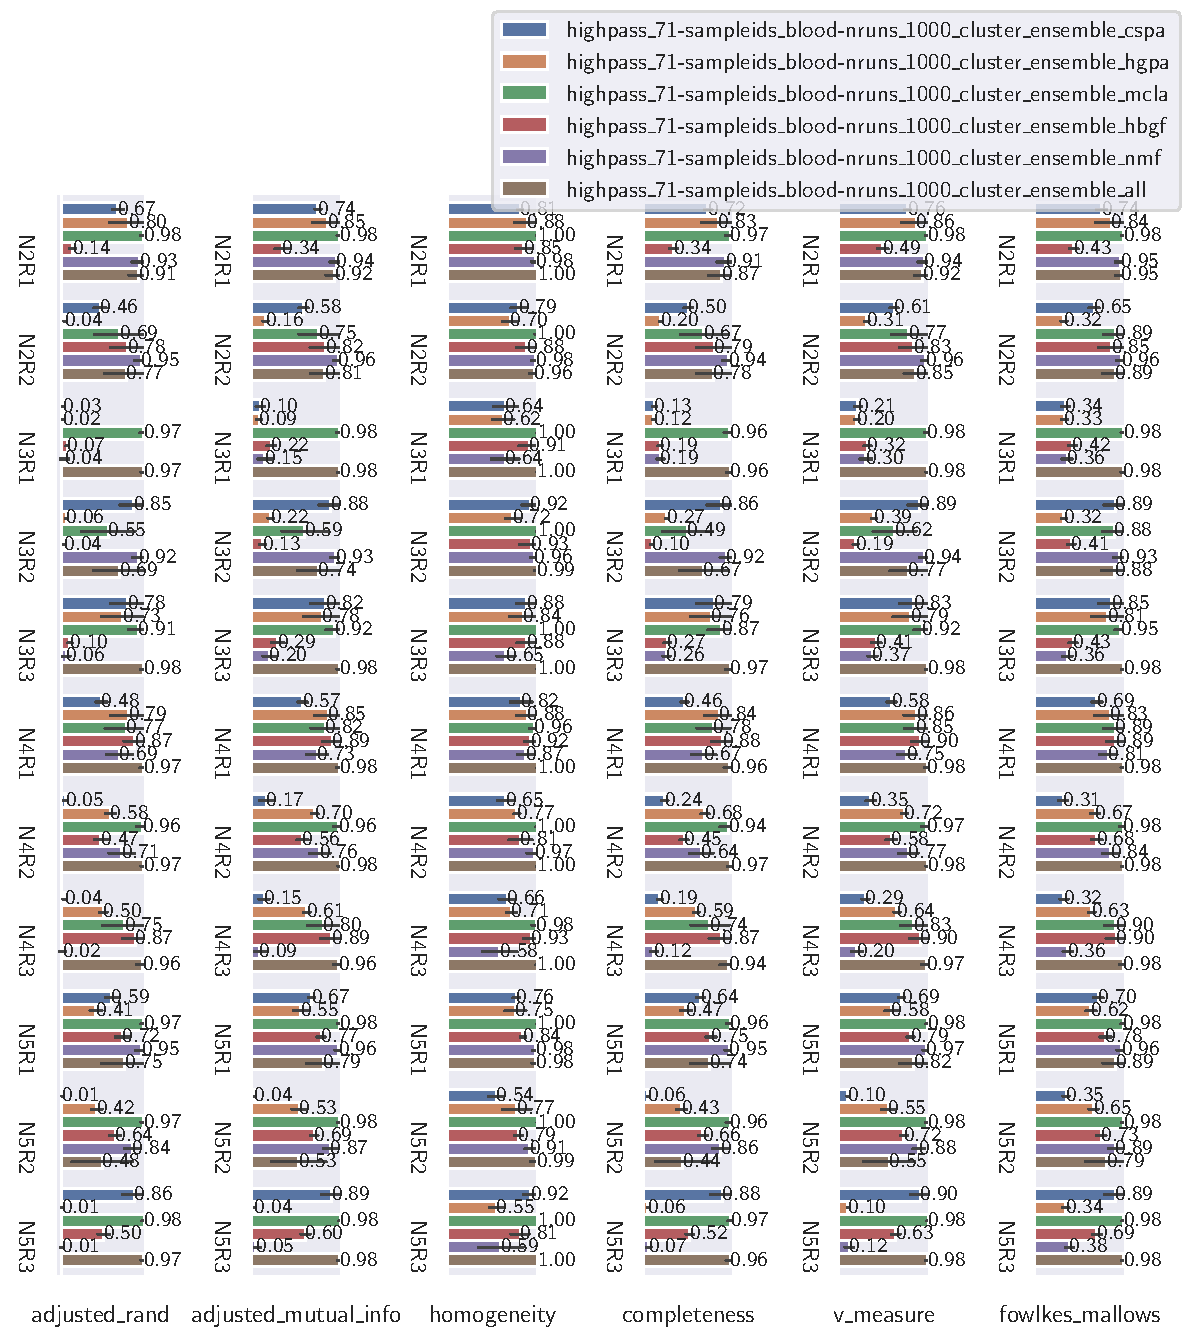
\includegraphics[width=\textwidth]{./figures/clust_comparison/highpass_71-sampleids_blood-nruns_1000_cluster_ensembles.pdf}
\caption{Cluster ensembles clustering performance metrics using 1000 trials sampled from EPGs from only blood samples with high-pass filtering}
\label{fig:highpass_71-sampleids_blood-nruns_1000_cluster_ensembles}
\end{figure}

\begin{table}[H]
\centering
\maxsizebox{\textwidth}{0.65\textwidth}{
\begin{tabular}{llrrrrrrrrrrrr}
\toprule
     & {} & \multicolumn{6}{l}{homogeneity} & \multicolumn{6}{l}{completeness} \\
     & clusterer &           1 &      2 &      3 &      4 &      5 &      6 &            1 &      2 &      3 &      4 &      5 &      6 \\
\midrule
N2R1 & ci\_upp &       0.38\% & 58.55\% & 97.72\% & 10.28\% & 84.35\% & 99.95\% &        0.38\% & 58.55\% & 68.97\% &  0.38\% & 55.28\% & 54.69\% \\
     & success &       0.00\% & 55.50\% & 96.80\% &  8.40\% & 82.10\% & 99.80\% &        0.00\% & 55.50\% & 66.10\% &  0.00\% & 52.20\% & 51.60\% \\
     & ci\_low &       0.00\% & 52.40\% & 95.52\% &  6.84\% & 79.60\% & 99.27\% &        0.00\% & 52.40\% & 63.11\% &  0.00\% & 49.10\% & 48.50\% \\
N2R2 & ci\_upp &       0.38\% &  0.38\% & 98.30\% & 49.80\% & 79.12\% & 63.19\% &        0.38\% &  0.38\% & 21.76\% & 49.80\% & 55.08\% & 17.03\% \\
     & success &       0.00\% &  0.00\% & 97.50\% & 46.70\% & 76.60\% & 60.20\% &        0.00\% &  0.00\% & 19.20\% & 46.70\% & 52.00\% & 14.70\% \\
     & ci\_low &       0.00\% &  0.00\% & 96.34\% & 43.63\% & 73.88\% & 57.13\% &        0.00\% &  0.00\% & 16.88\% & 43.63\% & 48.90\% & 12.64\% \\
N3R1 & ci\_upp &       0.38\% &  0.38\% & 98.70\% & 52.59\% &  0.38\% & 91.80\% &        0.38\% &  0.38\% & 69.36\% &  0.38\% &  0.38\% & 53.49\% \\
     & success &       0.00\% &  0.00\% & 98.00\% & 49.50\% &  0.00\% & 90.10\% &        0.00\% &  0.00\% & 66.50\% &  0.00\% &  0.00\% & 50.40\% \\
     & ci\_low &       0.00\% &  0.00\% & 96.93\% & 46.41\% &  0.00\% & 88.09\% &        0.00\% &  0.00\% & 63.52\% &  0.00\% &  0.00\% & 47.31\% \\
N3R2 & ci\_upp &      56.97\% &  0.38\% & 99.95\% & 74.21\% & 43.57\% & 97.39\% &       56.97\% &  0.38\% & 15.33\% &  0.38\% & 34.85\% & 21.76\% \\
     & success &      53.90\% &  0.00\% & 99.80\% & 71.50\% & 40.50\% & 96.40\% &       53.90\% &  0.00\% & 13.10\% &  0.00\% & 31.90\% & 19.20\% \\
     & ci\_low &      50.80\% &  0.00\% & 99.27\% & 68.62\% & 37.50\% & 95.06\% &       50.80\% &  0.00\% & 11.15\% &  0.00\% & 29.09\% & 16.88\% \\
N3R3 & ci\_upp &      49.80\% & 49.90\% & 99.95\% & 31.27\% &  0.38\% & 97.81\% &       49.80\% & 49.80\% & 54.39\% &  0.38\% &  0.38\% & 69.16\% \\
     & success &      46.70\% & 46.80\% & 99.80\% & 28.40\% &  0.00\% & 96.90\% &       46.70\% & 46.70\% & 51.30\% &  0.00\% &  0.00\% & 66.30\% \\
     & ci\_low &      43.63\% & 43.73\% & 99.27\% & 25.69\% &  0.00\% & 95.63\% &       43.63\% & 43.63\% & 48.20\% &  0.00\% &  0.00\% & 63.31\% \\
N4R1 & ci\_upp &      30.14\% & 53.89\% & 63.48\% & 38.72\% & 19.77\% & 98.70\% &        0.38\% & 53.89\% & 17.03\% & 38.72\% &  8.20\% & 69.36\% \\
     & success &      27.30\% & 50.80\% & 60.50\% & 35.70\% & 17.30\% & 98.00\% &        0.00\% & 50.80\% & 14.70\% & 35.70\% &  6.50\% & 66.50\% \\
     & ci\_low &      24.63\% & 47.70\% & 57.44\% & 32.79\% & 15.08\% & 96.93\% &        0.00\% & 47.70\% & 12.64\% & 32.79\% &  5.13\% & 63.52\% \\
N4R2 & ci\_upp &       0.38\% &  0.38\% & 97.64\% & 29.12\% & 88.20\% & 94.24\% &        0.38\% &  0.38\% & 72.37\% &  0.38\% &  5.06\% & 51.70\% \\
     & success &       0.00\% &  0.00\% & 96.70\% & 26.30\% & 86.20\% & 92.80\% &        0.00\% &  0.00\% & 69.60\% &  0.00\% &  3.70\% & 48.60\% \\
     & ci\_low &       0.00\% &  0.00\% & 95.40\% & 23.67\% & 83.92\% & 91.03\% &        0.00\% &  0.00\% & 66.68\% &  0.00\% &  2.70\% & 45.51\% \\
N4R3 & ci\_upp &       0.56\% &  0.38\% & 83.50\% & 56.97\% &  1.44\% & 97.64\% &        0.38\% &  0.38\% & 18.09\% & 56.97\% &  0.38\% & 72.47\% \\
     & success &       0.10\% &  0.00\% & 81.20\% & 53.90\% &  0.70\% & 96.70\% &        0.00\% &  0.00\% & 15.70\% & 53.90\% &  0.00\% & 69.70\% \\
     & ci\_low &       0.02\% &  0.00\% & 78.66\% & 50.80\% &  0.34\% & 95.40\% &        0.00\% &  0.00\% & 13.58\% & 50.80\% &  0.00\% & 66.78\% \\
N5R1 & ci\_upp &       0.38\% &  0.38\% & 91.89\% &  0.38\% & 74.89\% & 82.84\% &        0.38\% &  0.38\% & 53.29\% &  0.38\% & 46.49\% & 18.09\% \\
     & success &       0.00\% &  0.00\% & 90.20\% &  0.00\% & 72.20\% & 80.50\% &        0.00\% &  0.00\% & 50.20\% &  0.00\% & 43.40\% & 15.70\% \\
     & ci\_low &       0.00\% &  0.00\% & 88.20\% &  0.00\% & 69.34\% & 77.93\% &        0.00\% &  0.00\% & 47.11\% &  0.00\% & 40.36\% & 13.58\% \\
N5R2 & ci\_upp &       0.38\% & 31.89\% & 97.47\% &  0.38\% & 20.71\% & 96.88\% &        0.38\% &  0.38\% & 57.96\% &  0.38\% & 22.70\% & 14.80\% \\
     & success &       0.00\% & 29.00\% & 96.50\% &  0.00\% & 18.20\% & 95.80\% &        0.00\% &  0.00\% & 54.90\% &  0.00\% & 20.10\% & 12.60\% \\
     & ci\_low &       0.00\% & 26.27\% & 95.17\% &  0.00\% & 15.93\% & 94.37\% &        0.00\% &  0.00\% & 51.80\% &  0.00\% & 17.73\% & 10.69\% \\
N5R3 & ci\_upp &      51.70\% &  0.38\% & 97.22\% &  7.76\% & 26.23\% & 97.47\% &       51.70\% &  0.38\% & 52.10\% &  0.38\% &  0.38\% & 57.86\% \\
     & success &      48.60\% &  0.00\% & 96.20\% &  6.10\% & 23.50\% & 96.50\% &       48.60\% &  0.00\% & 49.00\% &  0.00\% &  0.00\% & 54.80\% \\
     & ci\_low &      45.51\% &  0.00\% & 94.83\% &  4.78\% & 20.98\% & 95.17\% &       45.51\% &  0.00\% & 45.91\% &  0.00\% &  0.00\% & 51.70\% \\
\bottomrule
\end{tabular}


}
\caption{Cluster ensembles clustering percentages of trials where no error occurs using 1000 trials sampled from EPGs from only blood samples with high-pass filtering}
\label{table:highpass_71-sampleids_blood-nruns_1000_cluster_ensembles}
\end{table}

\subsection{All Samples, without High-Pass Filtering}

\begin{figure}[H]
\centering
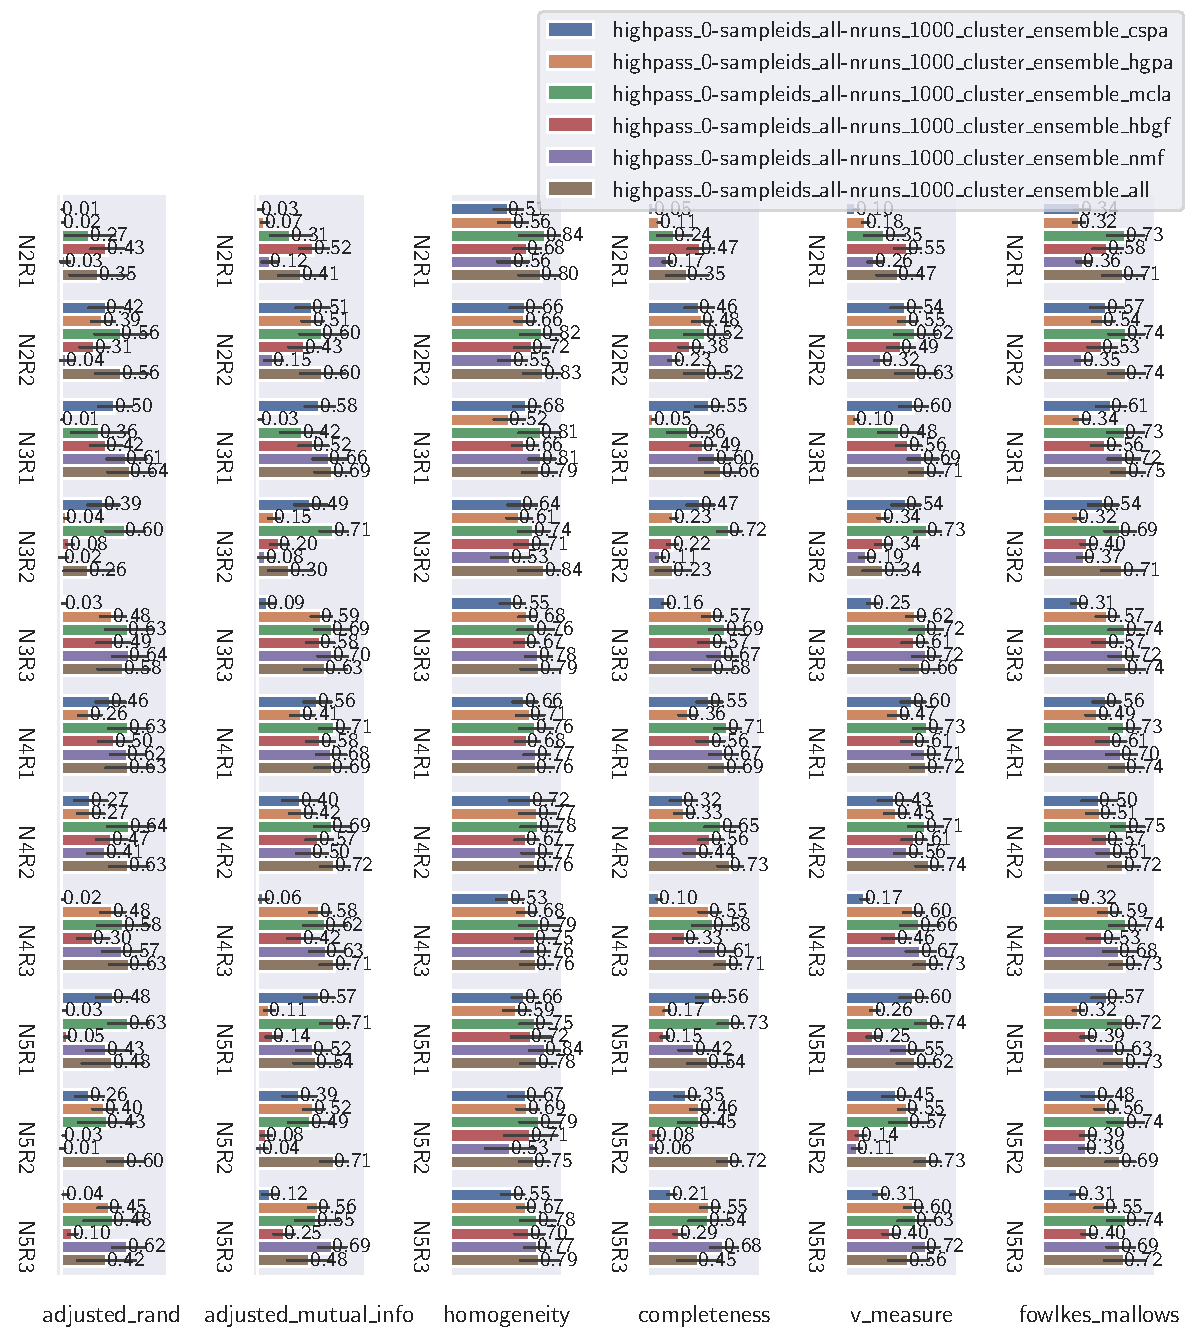
\includegraphics[width=\textwidth]{./figures/clust_comparison/highpass_0-sampleids_all-nruns_1000_cluster_ensembles.pdf}
\caption{Cluster ensembles clustering performance metrics using 1000 trials sampled from all EPGs without high-pass filtering}
\label{fig:highpass_0-sampleids_all-nruns_1000_cluster_ensembles}
\end{figure}

\begin{table}[H]
\centering
\maxsizebox{\textwidth}{0.65\textwidth}{
\begin{tabular}{llrrrrrrrrrrrr}
\toprule
     & {} & \multicolumn{6}{l}{homogeneity} & \multicolumn{6}{l}{completeness} \\
     & clusterer &           1 &      2 &      3 &      4 &      5 &      6 &            1 &     2 &     3 &     4 &     5 &     6 \\
\midrule
N2R1 & ci\_upp &       0.73\% &  1.02\% & 65.84\% &  0.73\% &  0.38\% & 37.40\% &        0.38\% & 0.38\% & 0.73\% & 0.38\% & 0.38\% & 1.02\% \\
     & success &       0.20\% &  0.40\% & 62.90\% &  0.20\% &  0.00\% & 34.40\% &        0.00\% & 0.00\% & 0.20\% & 0.00\% & 0.00\% & 0.40\% \\
     & ci\_low &       0.05\% &  0.16\% & 59.86\% &  0.05\% &  0.00\% & 31.52\% &        0.00\% & 0.00\% & 0.05\% & 0.00\% & 0.00\% & 0.16\% \\
N2R2 & ci\_upp &       0.88\% &  0.38\% & 32.91\% &  4.02\% &  0.38\% & 33.01\% &        0.38\% & 0.38\% & 3.31\% & 0.38\% & 0.38\% & 3.43\% \\
     & success &       0.30\% &  0.00\% & 30.00\% &  2.80\% &  0.00\% & 30.10\% &        0.00\% & 0.00\% & 2.20\% & 0.00\% & 0.00\% & 2.30\% \\
     & ci\_low &       0.10\% &  0.00\% & 27.24\% &  1.94\% &  0.00\% & 27.34\% &        0.00\% & 0.00\% & 1.46\% & 0.00\% & 0.00\% & 1.54\% \\
N3R1 & ci\_upp &       0.73\% &  2.58\% & 38.11\% &  0.56\% &  6.42\% &  7.09\% &        0.73\% & 0.38\% & 1.02\% & 0.38\% & 0.73\% & 1.17\% \\
     & success &       0.20\% &  1.60\% & 35.10\% &  0.10\% &  4.90\% &  5.50\% &        0.20\% & 0.00\% & 0.40\% & 0.00\% & 0.20\% & 0.50\% \\
     & ci\_low &       0.05\% &  0.99\% & 32.20\% &  0.02\% &  3.73\% &  4.25\% &        0.05\% & 0.00\% & 0.16\% & 0.00\% & 0.05\% & 0.21\% \\
N3R2 & ci\_upp &       0.38\% &  0.38\% &  0.38\% &  2.83\% &  1.83\% & 64.17\% &        0.38\% & 0.38\% & 0.38\% & 0.38\% & 0.38\% & 0.73\% \\
     & success &       0.00\% &  0.00\% &  0.00\% &  1.80\% &  1.00\% & 61.20\% &        0.00\% & 0.00\% & 0.00\% & 0.00\% & 0.00\% & 0.20\% \\
     & ci\_low &       0.00\% &  0.00\% &  0.00\% &  1.14\% &  0.54\% & 58.14\% &        0.00\% & 0.00\% & 0.00\% & 0.00\% & 0.00\% & 0.05\% \\
N3R3 & ci\_upp &       0.56\% &  0.38\% &  3.90\% &  0.38\% &  0.88\% & 18.19\% &        0.38\% & 0.38\% & 1.57\% & 0.38\% & 0.56\% & 4.25\% \\
     & success &       0.10\% &  0.00\% &  2.70\% &  0.00\% &  0.30\% & 15.80\% &        0.00\% & 0.00\% & 0.80\% & 0.00\% & 0.10\% & 3.00\% \\
     & ci\_low &       0.02\% &  0.00\% &  1.86\% &  0.00\% &  0.10\% & 13.67\% &        0.00\% & 0.00\% & 0.41\% & 0.00\% & 0.02\% & 2.11\% \\
N4R1 & ci\_upp &       0.38\% &  0.38\% &  1.02\% &  0.73\% &  0.73\% &  3.90\% &        0.56\% & 0.38\% & 0.73\% & 0.73\% & 0.56\% & 1.57\% \\
     & success &       0.00\% &  0.00\% &  0.40\% &  0.20\% &  0.20\% &  2.70\% &        0.10\% & 0.00\% & 0.20\% & 0.20\% & 0.10\% & 0.80\% \\
     & ci\_low &       0.00\% &  0.00\% &  0.16\% &  0.05\% &  0.05\% &  1.86\% &        0.02\% & 0.00\% & 0.05\% & 0.05\% & 0.02\% & 0.41\% \\
N4R2 & ci\_upp &      16.08\% & 21.76\% &  7.09\% &  0.38\% &  5.51\% &  0.88\% &        0.38\% & 0.38\% & 1.17\% & 0.56\% & 0.88\% & 0.73\% \\
     & success &      13.80\% & 19.20\% &  5.50\% &  0.00\% &  4.10\% &  0.30\% &        0.00\% & 0.00\% & 0.50\% & 0.10\% & 0.30\% & 0.20\% \\
     & ci\_low &      11.80\% & 16.88\% &  4.25\% &  0.00\% &  3.04\% &  0.10\% &        0.00\% & 0.00\% & 0.21\% & 0.02\% & 0.10\% & 0.05\% \\
N4R3 & ci\_upp &       0.38\% &  0.73\% & 18.19\% & 14.80\% &  1.83\% &  1.02\% &        0.38\% & 0.73\% & 4.25\% & 0.38\% & 0.56\% & 0.73\% \\
     & success &       0.00\% &  0.20\% & 15.80\% & 12.60\% &  1.00\% &  0.40\% &        0.00\% & 0.20\% & 3.00\% & 0.00\% & 0.10\% & 0.20\% \\
     & ci\_low &       0.00\% &  0.05\% & 13.67\% & 10.69\% &  0.54\% &  0.16\% &        0.00\% & 0.05\% & 2.11\% & 0.00\% & 0.02\% & 0.05\% \\
N5R1 & ci\_upp &       0.38\% &  0.38\% &  0.88\% & 11.69\% & 29.22\% & 11.91\% &        0.38\% & 0.38\% & 0.73\% & 0.38\% & 0.88\% & 1.57\% \\
     & success &       0.00\% &  0.00\% &  0.30\% &  9.70\% & 26.40\% &  9.90\% &        0.00\% & 0.00\% & 0.20\% & 0.00\% & 0.30\% & 0.80\% \\
     & ci\_low &       0.00\% &  0.00\% &  0.10\% &  8.02\% & 23.76\% &  8.20\% &        0.00\% & 0.00\% & 0.05\% & 0.00\% & 0.10\% & 0.41\% \\
N5R2 & ci\_upp &       0.38\% &  1.96\% & 19.77\% & 33.12\% & 15.65\% &  0.38\% &        0.38\% & 0.38\% & 0.88\% & 0.38\% & 0.38\% & 0.38\% \\
     & success &       0.00\% &  1.10\% & 17.30\% & 30.20\% & 13.40\% &  0.00\% &        0.00\% & 0.00\% & 0.30\% & 0.00\% & 0.00\% & 0.00\% \\
     & ci\_low &       0.00\% &  0.62\% & 15.08\% & 27.43\% & 11.43\% &  0.00\% &        0.00\% & 0.00\% & 0.10\% & 0.00\% & 0.00\% & 0.00\% \\
N5R3 & ci\_upp &       0.38\% &  0.38\% & 12.02\% &  1.57\% &  0.38\% & 18.82\% &        0.38\% & 0.56\% & 1.57\% & 0.38\% & 0.38\% & 0.88\% \\
     & success &       0.00\% &  0.00\% & 10.00\% &  0.80\% &  0.00\% & 16.40\% &        0.00\% & 0.10\% & 0.80\% & 0.00\% & 0.00\% & 0.30\% \\
     & ci\_low &       0.00\% &  0.00\% &  8.29\% &  0.41\% &  0.00\% & 14.23\% &        0.00\% & 0.02\% & 0.41\% & 0.00\% & 0.00\% & 0.10\% \\
\bottomrule
\end{tabular}


}
\caption{Cluster ensembles clustering percentages of trials where no error occurs using 1000 trials sampled from all EPGs without high-pass filtering}
\label{table:highpass_0-sampleids_all-nruns_1000_cluster_ensembles}
\end{table}

\subsection{All Samples, with High-Pass Filtering}

\begin{figure}[H]
\centering
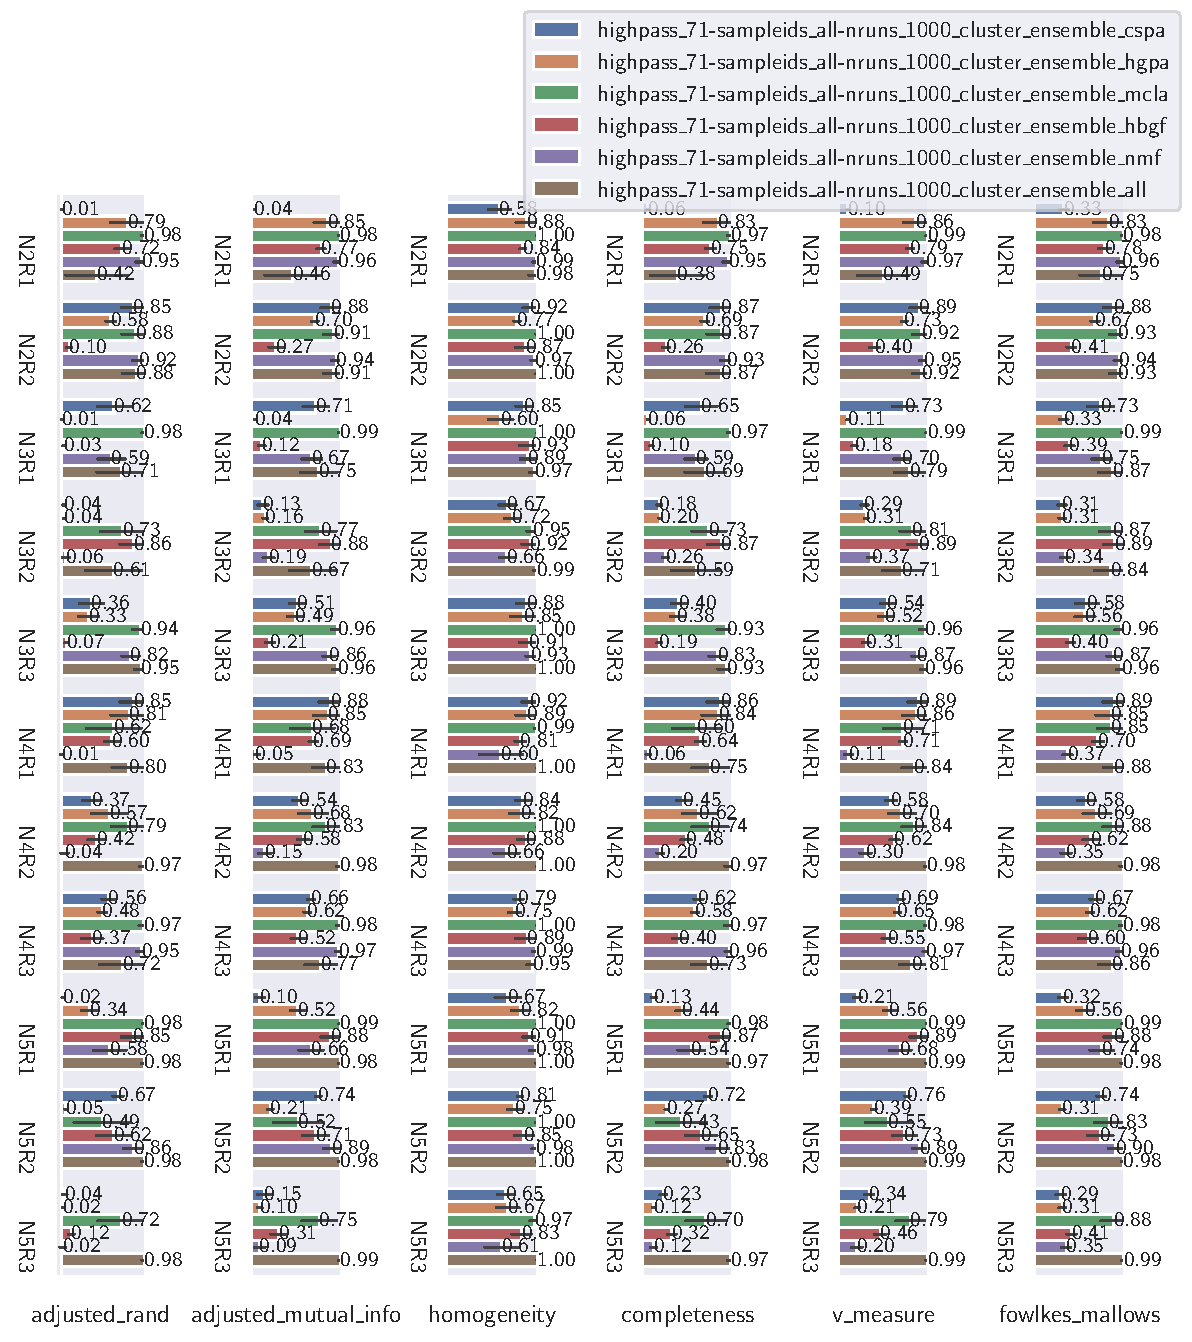
\includegraphics[width=\textwidth]{./figures/clust_comparison/highpass_71-sampleids_all-nruns_1000_cluster_ensembles.pdf}
\caption{Cluster ensembles clustering performance metrics using 1000 trials sampled from all EPGs with high-pass filtering}
\label{fig:highpass_71-sampleids_all-nruns_1000_cluster_ensembles}
\end{figure}

\begin{table}[H]
\centering
\maxsizebox{\textwidth}{0.65\textwidth}{
\begin{tabular}{llrrrrrrrrrrrr}
\toprule
     & {} & \multicolumn{6}{l}{homogeneity} & \multicolumn{6}{l}{completeness} \\
     & clusterer &           1 &      2 &      3 &      4 &      5 &      6 &            1 &      2 &      3 &      4 &      5 &      6 \\
\midrule
N2R1 & ci\_upp &       4.37\% & 51.40\% & 94.60\% &  0.38\% & 86.70\% & 95.05\% &        0.38\% & 51.40\% & 67.99\% &  0.38\% & 58.06\% & 10.72\% \\
     & success &       3.10\% & 48.30\% & 93.20\% &  0.00\% & 84.60\% & 93.70\% &        0.00\% & 48.30\% & 65.10\% &  0.00\% & 55.00\% &  8.80\% \\
     & ci\_low &       2.19\% & 45.22\% & 91.47\% &  0.00\% & 82.23\% & 92.02\% &        0.00\% & 45.22\% & 62.09\% &  0.00\% & 51.90\% &  7.20\% \\
N2R2 & ci\_upp &      50.20\% &  0.38\% & 98.78\% & 27.16\% & 53.69\% & 98.70\% &       50.20\% &  0.38\% & 56.27\% &  0.38\% & 36.48\% & 56.27\% \\
     & success &      47.10\% &  0.00\% & 98.10\% & 24.40\% & 50.60\% & 98.00\% &       47.10\% &  0.00\% & 53.20\% &  0.00\% & 33.50\% & 53.20\% \\
     & ci\_low &      44.02\% &  0.00\% & 97.05\% & 21.84\% & 47.50\% & 96.93\% &       44.02\% &  0.00\% & 50.10\% &  0.00\% & 30.64\% & 50.10\% \\
N3R1 & ci\_upp &      23.01\% &  8.09\% & 98.30\% & 75.18\% & 30.97\% & 71.79\% &       20.92\% &  0.38\% & 70.82\% &  0.38\% &  2.83\% & 10.39\% \\
     & success &      20.40\% &  6.40\% & 97.50\% & 72.50\% & 28.10\% & 69.00\% &       18.40\% &  0.00\% & 68.00\% &  0.00\% &  1.80\% &  8.50\% \\
     & ci\_low &      18.02\% &  5.04\% & 96.34\% & 69.65\% & 25.40\% & 66.07\% &       16.12\% &  0.00\% & 65.04\% &  0.00\% &  1.14\% &  6.93\% \\
N3R2 & ci\_upp &       0.38\% &  0.38\% & 52.89\% & 58.16\% &  0.38\% & 95.75\% &        0.38\% &  0.38\% &  8.53\% & 58.16\% &  0.38\% & 13.73\% \\
     & success &       0.00\% &  0.00\% & 49.80\% & 55.10\% &  0.00\% & 94.50\% &        0.00\% &  0.00\% &  6.80\% & 55.10\% &  0.00\% & 11.60\% \\
     & ci\_low &       0.00\% &  0.00\% & 46.71\% & 52.00\% &  0.00\% & 92.91\% &        0.00\% &  0.00\% &  5.40\% & 52.00\% &  0.00\% &  9.76\% \\
N3R3 & ci\_upp &      46.79\% & 43.57\% & 99.59\% & 52.30\% & 33.42\% & 99.59\% &        0.38\% &  0.38\% & 61.42\% &  0.38\% & 12.34\% & 61.61\% \\
     & success &      43.70\% & 40.50\% & 99.20\% & 49.20\% & 30.50\% & 99.20\% &        0.00\% &  0.00\% & 58.40\% &  0.00\% & 10.30\% & 58.60\% \\
     & ci\_low &      40.66\% & 37.50\% & 98.43\% & 46.11\% & 27.73\% & 98.43\% &        0.00\% &  0.00\% & 55.32\% &  0.00\% &  8.57\% & 55.52\% \\
N4R1 & ci\_upp &      58.16\% & 59.05\% & 96.88\% &  4.37\% & 25.09\% & 99.90\% &       58.16\% & 59.05\% & 13.73\% &  0.38\% &  0.38\% & 32.09\% \\
     & success &      55.10\% & 56.00\% & 95.80\% &  3.10\% & 22.40\% & 99.70\% &       55.10\% & 56.00\% & 11.60\% &  0.00\% &  0.00\% & 29.20\% \\
     & ci\_low &      52.00\% & 52.91\% & 94.37\% &  2.19\% & 19.92\% & 99.12\% &       52.00\% & 52.91\% &  9.76\% &  0.00\% &  0.00\% & 26.47\% \\
N4R2 & ci\_upp &       0.56\% & 34.45\% & 99.90\% & 25.81\% &  0.38\% & 97.89\% &        0.38\% & 20.92\% & 31.99\% &  0.38\% &  0.38\% & 72.66\% \\
     & success &       0.10\% & 31.50\% & 99.70\% & 23.10\% &  0.00\% & 97.00\% &        0.00\% & 18.40\% & 29.10\% &  0.00\% &  0.00\% & 69.90\% \\
     & ci\_low &       0.02\% & 28.70\% & 99.12\% & 20.59\% &  0.00\% & 95.75\% &        0.00\% & 16.12\% & 26.37\% &  0.00\% &  0.00\% & 66.99\% \\
N4R3 & ci\_upp &       0.38\% &  0.38\% & 97.72\% & 50.30\% & 82.36\% & 52.50\% &        0.38\% &  0.38\% & 72.57\% &  0.38\% & 47.70\% &  8.53\% \\
     & success &       0.00\% &  0.00\% & 96.80\% & 47.20\% & 80.00\% & 49.40\% &        0.00\% &  0.00\% & 69.80\% &  0.00\% & 44.60\% &  6.80\% \\
     & ci\_low &       0.00\% &  0.00\% & 95.52\% & 44.12\% & 77.41\% & 46.31\% &        0.00\% &  0.00\% & 66.88\% &  0.00\% & 41.55\% &  5.40\% \\
N5R1 & ci\_upp &       2.09\% &  1.02\% & 97.39\% & 36.08\% & 92.89\% & 94.60\% &        0.38\% &  0.38\% & 61.81\% & 36.08\% &  2.58\% & 61.52\% \\
     & success &       1.20\% &  0.40\% & 96.40\% & 33.10\% & 91.30\% & 93.20\% &        0.00\% &  0.00\% & 58.80\% & 33.10\% &  1.60\% & 58.50\% \\
     & ci\_low &       0.69\% &  0.16\% & 95.06\% & 30.25\% & 89.39\% & 91.47\% &        0.00\% &  0.00\% & 55.72\% & 30.25\% &  0.99\% & 55.42\% \\
N5R2 & ci\_upp &       0.38\% &  0.38\% & 99.90\% & 25.61\% & 88.20\% & 94.87\% &        0.38\% &  0.38\% & 10.93\% & 20.92\% & 25.19\% & 68.19\% \\
     & success &       0.00\% &  0.00\% & 99.70\% & 22.90\% & 86.20\% & 93.50\% &        0.00\% &  0.00\% &  9.00\% & 18.40\% & 22.50\% & 65.30\% \\
     & ci\_low &       0.00\% &  0.00\% & 99.12\% & 20.40\% & 83.92\% & 91.80\% &        0.00\% &  0.00\% &  7.38\% & 16.12\% & 20.02\% & 62.30\% \\
N5R3 & ci\_upp &       0.38\% &  1.70\% & 72.66\% &  9.41\% &  2.58\% & 98.46\% &        0.38\% &  0.38\% & 10.39\% &  0.38\% &  0.38\% & 71.11\% \\
     & success &       0.00\% &  0.90\% & 69.90\% &  7.60\% &  1.60\% & 97.70\% &        0.00\% &  0.00\% &  8.50\% &  0.00\% &  0.00\% & 68.30\% \\
     & ci\_low &       0.00\% &  0.47\% & 66.99\% &  6.11\% &  0.99\% & 96.57\% &        0.00\% &  0.00\% &  6.93\% &  0.00\% &  0.00\% & 65.35\% \\
\bottomrule
\end{tabular}


}
\caption{Cluster ensembles clustering percentages of trials where no error occurs using 1000 trials sampled from all EPGs with high-pass filtering}
\label{table:highpass_71-sampleids_all-nruns_1000_cluster_ensembles}
\end{table}

%--------------------------------------------------------------------------------------------------------------------------------------------
\section{Experiments Results---Overall}

\subsection{Saliva Samples Only, without High-Pass Filtering}

\begin{table}[H]
\centering
\maxsizebox{\textwidth}{0.65\textwidth}{
\begin{tabular}{lrr}
\toprule
{} &      mean &       std \\
clusterer                                          &           &           \\
\midrule
affinity\_l2\_norm                                   &  0.537845 &  0.193364 \\
hdbscan\_cosine\_epsilon\_0.0\_eom\_per\_locus\_norm      &  0.494584 &  0.274283 \\
hdbscan\_cosine\_epsilon\_0.0\_eom\_per\_locus\_quantize  &  0.486221 &  0.265297 \\
hdbscan\_cosine\_epsilon\_0.5\_leaf\_per\_locus\_norm     &  0.484973 &  0.267075 \\
hdbscan\_cosine\_epsilon\_0.5\_eom\_per\_locus\_norm      &  0.484847 &  0.271220 \\
affinity\_l1\_norm                                   &  0.473349 &  0.236314 \\
hdbscan\_euclidean\_epsilon\_0.5\_eom\_l2\_norm          &  0.464676 &  0.261550 \\
hdbscan\_euclidean\_epsilon\_0.0\_eom\_l2\_norm          &  0.464474 &  0.261570 \\
birch\_per\_locus\_norm                               &  0.461531 &  0.176776 \\
birch\_per\_locus\_quantize                           &  0.461388 &  0.176951 \\
hdbscan\_cosine\_epsilon\_0.0\_eom                     &  0.457188 &  0.258795 \\
birch\_l2\_norm                                      &  0.450668 &  0.201137 \\
hdbscan\_cosine\_epsilon\_0.0\_leaf\_per\_locus\_norm     &  0.447478 &  0.262407 \\
hdbscan\_euclidean\_epsilon\_0.5\_leaf\_l2\_norm         &  0.444169 &  0.259896 \\
cluster\_ensemble\_all                               &  0.438486 &  0.169205 \\
affinity\_per\_locus\_quantize                        &  0.438395 &  0.174343 \\
cluster\_ensemble\_mcla                              &  0.437384 &  0.166572 \\
meanshift\_per\_locus\_norm                           &  0.431335 &  0.263610 \\
affinity\_per\_locus\_norm                            &  0.429782 &  0.173224 \\
meanshift\_per\_locus\_quantize                       &  0.429451 &  0.259660 \\
hdbscan\_cosine\_epsilon\_0.0\_leaf\_per\_locus\_quantize &  0.429403 &  0.250309 \\
hdbscan\_euclidean\_epsilon\_0.0\_leaf\_l2\_norm         &  0.428211 &  0.254899 \\
optics\_l2\_norm                                     &  0.414122 &  0.255132 \\
hdbscan\_cosine\_epsilon\_0.0\_leaf                    &  0.409896 &  0.247945 \\
hdbscan\_euclidean\_epsilon\_1.0\_leaf\_l2\_norm         &  0.401358 &  0.250626 \\
\bottomrule
\end{tabular}


}
\caption{Top 25 clusterers, including ensembles, by arithmetic mean of clustering metric scores, using admixtures sampled from only saliva EPG data without highpass filter}
\label{table:top_25_clusterers_by_metrics_highpass_0-sampleids_saliva-nruns_1000}
\end{table}

\begin{figure}[H]
\centering
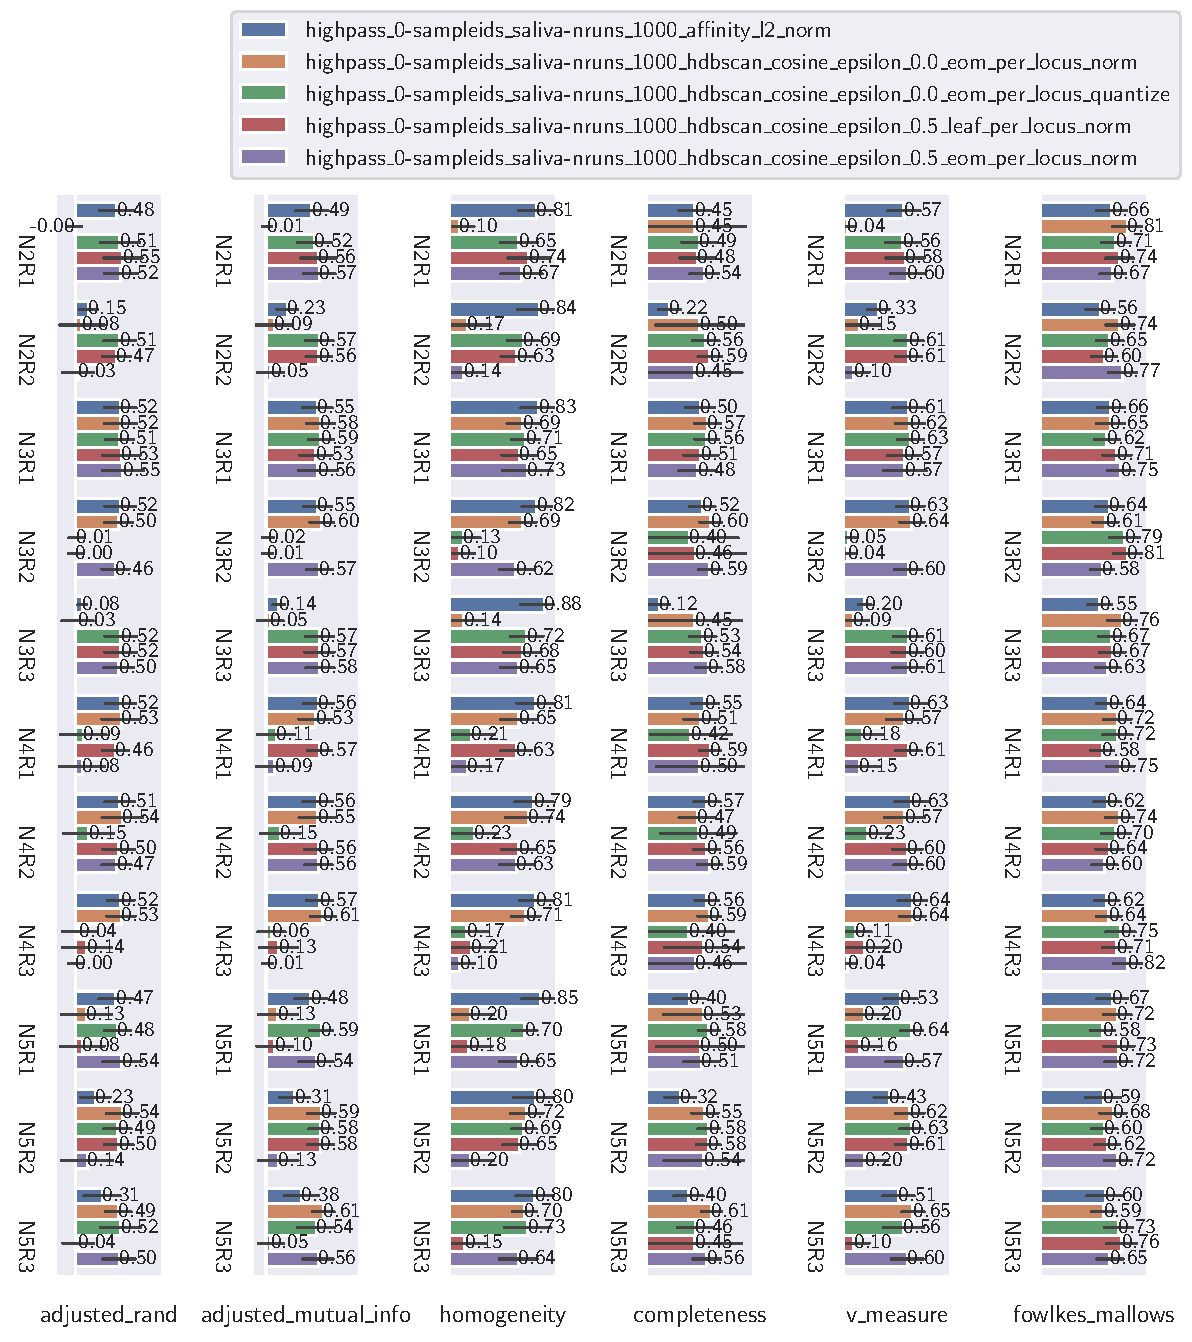
\includegraphics[width=\textwidth]{./figures/clust_comparison/highpass_0-sampleids_saliva-nruns_1000_top_5_clusterers_including_ensembles_by_metrics.pdf}
\caption{Top 5 clusterers, including ensembles, clustering performance metrics using 1000 trials sampled from EPGs from only saliva samples without high-pass filtering}
\label{fig:highpass_0-sampleids_saliva-nruns_1000_top_5_clusterers_including_ensembles_by_metrics}
\end{figure}

\begin{table}[H]
\centering
\maxsizebox{\textwidth}{0.65\textwidth}{
\begin{tabular}{lrr}
\toprule
{} &  mean &   std \\
clusterer                                         &       &       \\
\midrule
meanshift\_per\_locus\_norm                          & 1.13\% & 2.13\% \\
meanshift\_per\_locus\_quantize                      & 1.03\% & 2.05\% \\
birch\_l2\_norm                                     & 0.21\% & 0.27\% \\
hdbscan\_cosine\_epsilon\_1.0\_eom\_per\_locus\_norm     & 0.18\% & 0.25\% \\
hdbscan\_cosine\_epsilon\_1.0\_leaf\_per\_locus\_norm    & 0.18\% & 0.25\% \\
mclust\_l2\_norm                                    & 0.18\% & 0.28\% \\
hdbscan\_cosine\_epsilon\_0.0\_eom\_per\_locus\_norm     & 0.17\% & 0.24\% \\
hdbscan\_cosine\_epsilon\_0.5\_eom\_per\_locus\_norm     & 0.17\% & 0.24\% \\
hdbscan\_cosine\_epsilon\_0.5\_leaf\_per\_locus\_norm    & 0.17\% & 0.24\% \\
optics\_l2\_norm                                    & 0.16\% & 0.22\% \\
hdbscan\_cosine\_epsilon\_0.5\_eom                    & 0.16\% & 0.24\% \\
hdbscan\_cosine\_epsilon\_0.5\_leaf                   & 0.16\% & 0.24\% \\
hdbscan\_cosine\_epsilon\_1.0\_eom                    & 0.16\% & 0.24\% \\
hdbscan\_cosine\_epsilon\_1.0\_leaf                   & 0.16\% & 0.24\% \\
hdbscan\_euclidean\_epsilon\_1.0\_eom\_l2\_norm         & 0.16\% & 0.24\% \\
hdbscan\_euclidean\_epsilon\_1.0\_leaf\_l2\_norm        & 0.16\% & 0.24\% \\
hdbscan\_cosine\_epsilon\_0.0\_eom\_per\_locus\_quantize & 0.15\% & 0.21\% \\
hdbscan\_cosine\_epsilon\_0.0\_leaf\_per\_locus\_norm    & 0.15\% & 0.21\% \\
hdbscan\_cosine\_epsilon\_0.0\_eom                    & 0.15\% & 0.22\% \\
hdbscan\_euclidean\_epsilon\_0.0\_eom\_l2\_norm         & 0.15\% & 0.22\% \\
hdbscan\_euclidean\_epsilon\_0.5\_eom\_l2\_norm         & 0.15\% & 0.22\% \\
optics\_per\_locus\_norm                             & 0.15\% & 0.22\% \\
optics\_per\_locus\_quantize                         & 0.15\% & 0.22\% \\
hdbscan\_cosine\_epsilon\_0.0\_leaf                   & 0.15\% & 0.20\% \\
hdbscan\_euclidean\_epsilon\_0.0\_leaf\_l2\_norm        & 0.15\% & 0.20\% \\
\bottomrule
\end{tabular}


}
\caption{Top 25 clusterers by arithmetic mean of percentages of perfect clustering, using admixtures sampled from only saliva EPG data without highpass filter}
\label{table:top_25_clusterers_by_binomial_confidence_highpass_0-sampleids_saliva-nruns_1000}
\end{table}

\begin{table}[H]
\centering
\maxsizebox{\textwidth}{0.65\textwidth}{
\begin{tabular}{llrrrrrrrrrr}
\toprule
     & {} & \multicolumn{5}{l}{homogeneity} & \multicolumn{5}{l}{completeness} \\
     & clusterer &           1 &      2 &      3 &      4 &      5 &            1 &      2 &     3 &      4 &      5 \\
\midrule
N2R1 & ci\_upp &       0.38\% &  3.19\% &  0.38\% &  0.38\% &  0.38\% &       42.67\% & 14.16\% & 0.73\% & 39.43\% &  0.38\% \\
     & success &       0.00\% &  2.10\% &  0.00\% &  0.00\% &  0.00\% &       39.60\% & 12.00\% & 0.20\% & 36.40\% &  0.00\% \\
     & ci\_low &       0.00\% &  1.38\% &  0.00\% &  0.00\% &  0.00\% &       36.61\% & 10.13\% & 0.05\% & 33.48\% &  0.00\% \\
N2R2 & ci\_upp &       0.38\% &  0.38\% &  0.38\% &  0.38\% & 10.83\% &       56.18\% & 32.61\% & 1.30\% &  0.38\% &  0.88\% \\
     & success &       0.00\% &  0.00\% &  0.00\% &  0.00\% &  8.90\% &       53.10\% & 29.70\% & 0.60\% &  0.00\% &  0.30\% \\
     & ci\_low &       0.00\% &  0.00\% &  0.00\% &  0.00\% &  7.29\% &       50.00\% & 26.95\% & 0.28\% &  0.00\% &  0.10\% \\
N3R1 & ci\_upp &       0.38\% & 22.07\% &  0.38\% &  0.56\% &  0.38\% &       35.16\% & 10.28\% & 0.38\% & 45.99\% & 40.85\% \\
     & success &       0.00\% & 19.50\% &  0.00\% &  0.10\% &  0.00\% &       32.20\% &  8.40\% & 0.00\% & 42.90\% & 37.80\% \\
     & ci\_low &       0.00\% & 17.16\% &  0.00\% &  0.02\% &  0.00\% &       29.38\% &  6.84\% & 0.00\% & 39.87\% & 34.85\% \\
N3R2 & ci\_upp &       0.38\% &  0.38\% &  0.38\% &  1.02\% &  1.02\% &       54.88\% & 52.40\% & 0.38\% &  1.57\% &  1.57\% \\
     & success &       0.00\% &  0.00\% &  0.00\% &  0.40\% &  0.40\% &       51.80\% & 49.30\% & 0.00\% &  0.80\% &  0.80\% \\
     & ci\_low &       0.00\% &  0.00\% &  0.00\% &  0.16\% &  0.16\% &       48.70\% & 46.21\% & 0.00\% &  0.41\% &  0.41\% \\
N3R3 & ci\_upp &       6.98\% &  1.57\% &  1.02\% &  0.38\% &  0.38\% &        8.53\% & 12.66\% & 1.02\% &  0.38\% &  0.38\% \\
     & success &       5.40\% &  0.80\% &  0.40\% &  0.00\% &  0.00\% &        6.80\% & 10.60\% & 0.40\% &  0.00\% &  0.00\% \\
     & ci\_low &       4.16\% &  0.41\% &  0.16\% &  0.00\% &  0.00\% &        5.40\% &  8.84\% & 0.16\% &  0.00\% &  0.00\% \\
N4R1 & ci\_upp &       3.31\% &  0.38\% &  0.88\% &  0.38\% &  0.38\% &       19.24\% & 40.54\% & 0.88\% &  0.38\% &  0.38\% \\
     & success &       2.20\% &  0.00\% &  0.30\% &  0.00\% &  0.00\% &       16.80\% & 37.50\% & 0.30\% &  0.00\% &  0.00\% \\
     & ci\_low &       1.46\% &  0.00\% &  0.10\% &  0.00\% &  0.00\% &       14.61\% & 34.55\% & 0.10\% &  0.00\% &  0.00\% \\
N4R2 & ci\_upp &       1.02\% &  0.38\% &  0.38\% & 10.83\% &  0.56\% &       13.84\% & 43.17\% & 0.38\% &  0.88\% & 45.99\% \\
     & success &       0.40\% &  0.00\% &  0.00\% &  8.90\% &  0.10\% &       11.70\% & 40.10\% & 0.00\% &  0.30\% & 42.90\% \\
     & ci\_low &       0.16\% &  0.00\% &  0.00\% &  7.29\% &  0.02\% &        9.85\% & 37.11\% & 0.00\% &  0.10\% & 39.87\% \\
N4R3 & ci\_upp &       0.38\% &  5.40\% &  0.38\% &  0.38\% &  0.38\% &       43.88\% &  4.71\% & 0.38\% & 40.85\% & 36.18\% \\
     & success &       0.00\% &  4.00\% &  0.00\% &  0.00\% &  0.00\% &       40.80\% &  3.40\% & 0.00\% & 37.80\% & 33.20\% \\
     & ci\_low &       0.00\% &  2.95\% &  0.00\% &  0.00\% &  0.00\% &       37.79\% &  2.44\% & 0.00\% & 34.85\% & 30.35\% \\
N5R1 & ci\_upp &       2.09\% & 10.50\% &  9.30\% &  0.38\% &  0.38\% &        6.08\% &  7.20\% & 0.38\% & 36.18\% & 39.43\% \\
     & success &       1.20\% &  8.60\% &  7.50\% &  0.00\% &  0.00\% &        4.60\% &  5.60\% & 0.00\% & 33.20\% & 36.40\% \\
     & ci\_low &       0.69\% &  7.02\% &  6.03\% &  0.00\% &  0.00\% &        3.47\% &  4.34\% & 0.00\% & 30.35\% & 33.48\% \\
N5R2 & ci\_upp &      19.45\% &  0.38\% &  0.38\% &  0.38\% &  0.38\% &       12.45\% & 54.19\% & 0.56\% &  0.38\% &  0.38\% \\
     & success &      17.00\% &  0.00\% &  0.00\% &  0.00\% &  0.00\% &       10.40\% & 51.10\% & 0.10\% &  0.00\% &  0.00\% \\
     & ci\_low &      14.80\% &  0.00\% &  0.00\% &  0.00\% &  0.00\% &        8.66\% & 48.00\% & 0.02\% &  0.00\% &  0.00\% \\
N5R3 & ci\_upp &      44.08\% & 47.60\% & 12.77\% &  0.38\% &  0.38\% &       15.12\% & 14.37\% & 0.73\% &  0.38\% &  0.38\% \\
     & success &      41.00\% & 44.50\% & 10.70\% &  0.00\% &  0.00\% &       12.90\% & 12.20\% & 0.20\% &  0.00\% &  0.00\% \\
     & ci\_low &      37.99\% & 41.45\% &  8.93\% &  0.00\% &  0.00\% &       10.96\% & 10.31\% & 0.05\% &  0.00\% &  0.00\% \\
\bottomrule
\end{tabular}


}
\caption{Top 5 clusterers, including ensembles, clustering percentages of trials where no error occurs using 1000 trials sampled from EPGs from only saliva samples without high-pass filtering}
\label{table:highpass_0-sampleids_saliva-nruns_1000_top_5_clusterers_including_ensembles_by_binomial_confidence}
\end{table}

\subsection{Saliva Samples Only, with High-Pass Filtering}

\begin{table}[H]
\centering
\maxsizebox{\textwidth}{0.65\textwidth}{
\begin{tabular}{lrr}
\toprule
{} &      mean &       std \\
clusterer                                          &           &           \\
\midrule
mclust\_l2\_norm                                     &  0.896614 &  0.186136 \\
mclust\_l1\_norm                                     &  0.872849 &  0.196642 \\
birch\_per\_locus\_quantize                           &  0.869840 &  0.170125 \\
birch\_per\_locus\_norm                               &  0.869058 &  0.173117 \\
cluster\_ensemble\_mcla                              &  0.838775 &  0.235953 \\
birch\_l2\_norm                                      &  0.835254 &  0.195881 \\
affinity\_per\_locus\_quantize                        &  0.834774 &  0.260209 \\
cluster\_ensemble\_all                               &  0.832766 &  0.247135 \\
affinity\_per\_locus\_norm                            &  0.812169 &  0.271186 \\
affinity\_l1\_norm                                   &  0.805911 &  0.269273 \\
affinity\_l2\_norm                                   &  0.804455 &  0.281211 \\
hdbscan\_euclidean\_epsilon\_0.5\_eom\_l2\_norm          &  0.797744 &  0.354691 \\
hdbscan\_euclidean\_epsilon\_0.0\_eom\_l2\_norm          &  0.797697 &  0.354794 \\
hdbscan\_euclidean\_epsilon\_0.5\_leaf\_l2\_norm         &  0.794639 &  0.353828 \\
hdbscan\_cosine\_epsilon\_0.0\_eom                     &  0.793644 &  0.356433 \\
hdbscan\_euclidean\_epsilon\_0.0\_eom\_per\_locus\_qua... &  0.784172 &  0.366174 \\
hdbscan\_cosine\_epsilon\_0.0\_eom\_per\_locus\_norm      &  0.777161 &  0.374257 \\
hdbscan\_euclidean\_epsilon\_1.0\_eom\_per\_locus\_norm   &  0.775940 &  0.375626 \\
hdbscan\_euclidean\_epsilon\_0.5\_eom\_per\_locus\_norm   &  0.775929 &  0.375646 \\
hdbscan\_euclidean\_epsilon\_0.0\_eom\_per\_locus\_norm   &  0.775929 &  0.375646 \\
hdbscan\_euclidean\_epsilon\_0.0\_eom\_l1\_norm          &  0.759145 &  0.373824 \\
hdbscan\_euclidean\_epsilon\_0.0\_leaf\_l2\_norm         &  0.740871 &  0.356075 \\
hdbscan\_euclidean\_epsilon\_0.0\_leaf\_per\_locus\_qu... &  0.728092 &  0.361066 \\
hdbscan\_cosine\_epsilon\_0.5\_eom\_per\_locus\_norm      &  0.718517 &  0.358609 \\
hdbscan\_cosine\_epsilon\_0.5\_leaf\_per\_locus\_norm     &  0.718512 &  0.358615 \\
\bottomrule
\end{tabular}


}
\caption{Top 25 clusterers, including ensembles, by arithmetic mean of clustering metric scores, using admixtures sampled from only saliva EPG data with highpass filter}
\label{table:top_25_clusterers_by_metrics_highpass_71-sampleids_saliva-nruns_1000}
\end{table}

\begin{figure}[H]
\centering
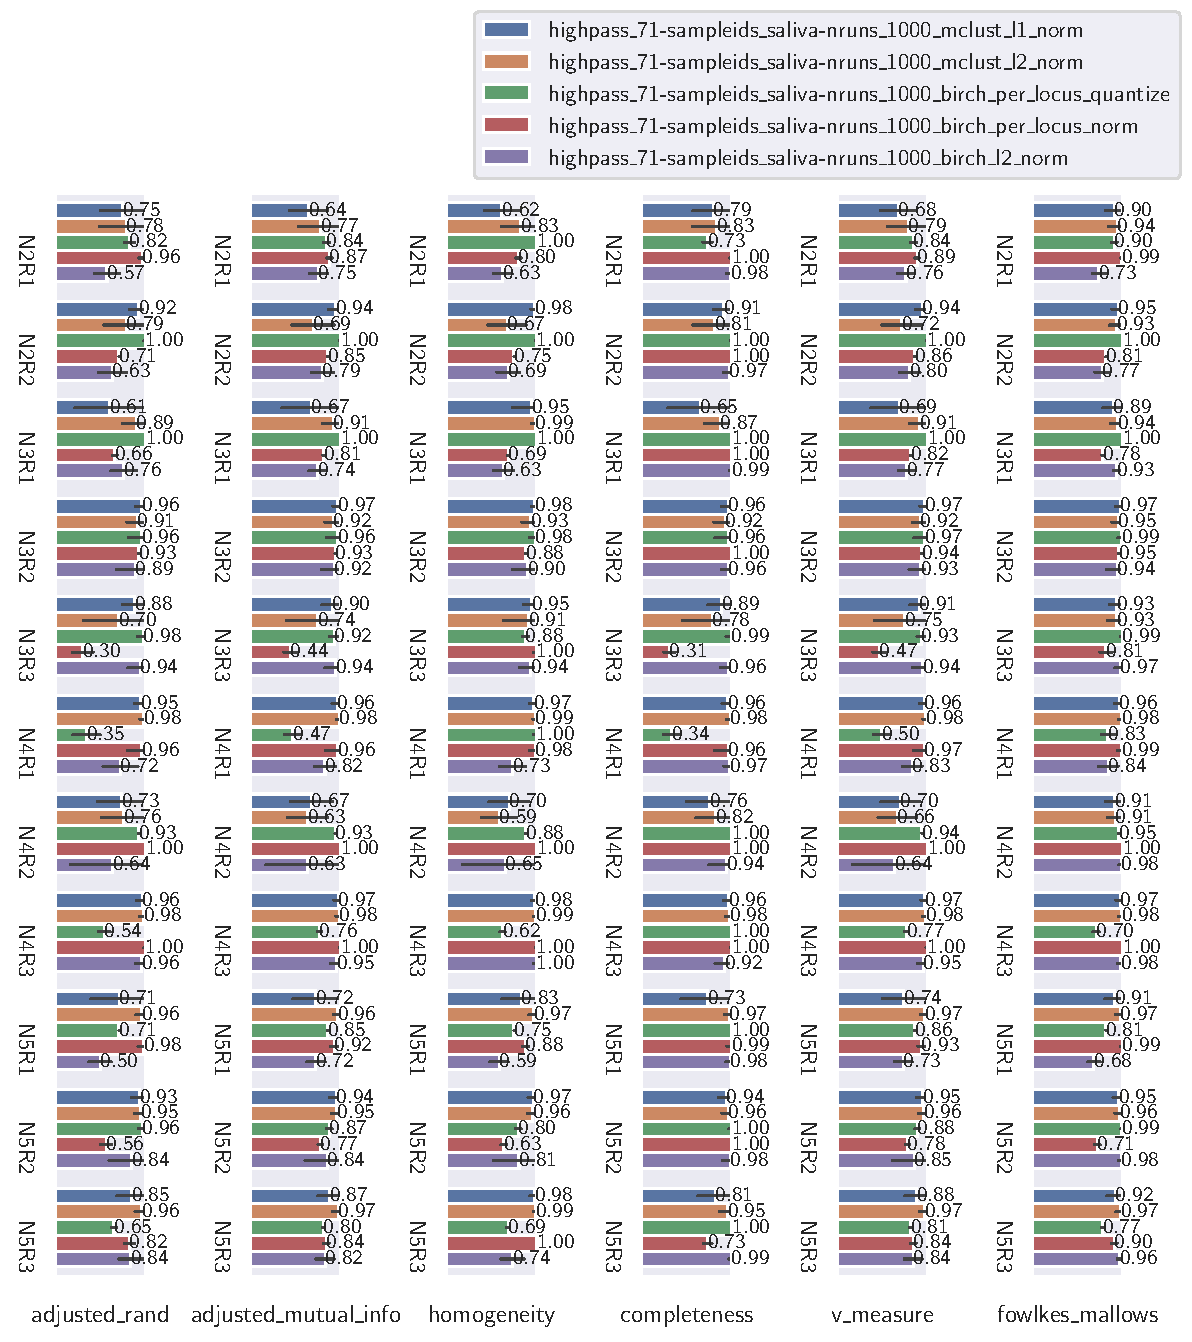
\includegraphics[width=\textwidth]{./figures/clust_comparison/highpass_71-sampleids_saliva-nruns_1000_top_5_clusterers_including_ensembles_by_metrics.pdf}
\caption{Top 5 clusterers, including ensembles, clustering performance metrics using 1000 trials sampled from EPGs from only saliva samples with high-pass filtering}
\label{fig:highpass_71-sampleids_saliva-nruns_1000_top_5_clusterers_including_ensembles_by_metrics}
\end{figure}

\begin{table}[H]
\centering
\maxsizebox{\textwidth}{0.65\textwidth}{
\begin{tabular}{lrr}
\toprule
{} &   mean &    std \\
clusterer                                          &        &        \\
\midrule
hdbscan\_euclidean\_epsilon\_0.0\_eom\_per\_locus\_norm   & 59.08\% & 46.44\% \\
hdbscan\_euclidean\_epsilon\_1.0\_eom\_per\_locus\_norm   & 59.08\% & 46.44\% \\
hdbscan\_euclidean\_epsilon\_0.5\_eom\_per\_locus\_norm   & 59.08\% & 46.44\% \\
hdbscan\_cosine\_epsilon\_0.0\_eom\_per\_locus\_norm      & 58.84\% & 46.75\% \\
hdbscan\_euclidean\_epsilon\_0.0\_eom\_per\_locus\_qua... & 57.91\% & 45.62\% \\
hdbscan\_euclidean\_epsilon\_0.5\_eom\_l2\_norm          & 52.04\% & 41.79\% \\
hdbscan\_euclidean\_epsilon\_0.0\_eom\_l2\_norm          & 52.04\% & 41.79\% \\
hdbscan\_cosine\_epsilon\_0.0\_eom                     & 50.17\% & 40.41\% \\
affinity\_per\_locus\_quantize                        & 49.54\% & 38.19\% \\
hdbscan\_euclidean\_epsilon\_0.5\_leaf\_l2\_norm         & 49.15\% & 39.64\% \\
affinity\_l2\_norm                                   & 48.82\% & 37.70\% \\
mclust\_l2\_norm                                     & 47.68\% & 24.86\% \\
affinity\_per\_locus\_norm                            & 46.21\% & 35.75\% \\
cluster\_ensemble\_all                               & 45.55\% & 40.34\% \\
cluster\_ensemble\_mcla                              & 45.28\% & 40.03\% \\
mclust\_l1\_norm                                     & 41.23\% & 20.33\% \\
affinity\_l1\_norm                                   & 38.91\% & 30.07\% \\
optics\_per\_locus\_quantize                          & 35.55\% & 28.93\% \\
hdbscan\_cosine\_epsilon\_0.5\_leaf\_per\_locus\_norm     & 35.12\% & 32.36\% \\
hdbscan\_cosine\_epsilon\_0.5\_eom\_per\_locus\_norm      & 35.12\% & 32.36\% \\
hdbscan\_cosine\_epsilon\_0.0\_eom\_per\_locus\_quantize  & 33.74\% & 27.15\% \\
hdbscan\_euclidean\_epsilon\_0.0\_leaf\_per\_locus\_qu... & 30.83\% & 24.99\% \\
hdbscan\_euclidean\_epsilon\_0.0\_eom\_l1\_norm          & 30.71\% & 27.52\% \\
hdbscan\_euclidean\_epsilon\_0.0\_leaf\_l2\_norm         & 30.69\% & 25.85\% \\
birch\_l2\_norm                                      & 29.69\% & 33.32\% \\
\bottomrule
\end{tabular}


}
\caption{Top 25 clusterers by arithmetic mean of percentages of perfect clustering, using admixtures sampled from only saliva EPG data with highpass filter}
\label{table:top_25_clusterers_by_binomial_confidence_highpass_71-sampleids_saliva-nruns_1000}
\end{table}

\begin{table}[H]
\centering
\maxsizebox{\textwidth}{0.65\textwidth}{
\begin{tabular}{llrrrrrrrrrr}
\toprule
     & {} & \multicolumn{5}{l}{homogeneity} & \multicolumn{5}{l}{completeness} \\
     & clusterer &           1 &       2 &       3 &       4 &       5 &            1 &      2 &      3 &      4 &      5 \\
\midrule
N2R1 & ci\_upp &     100.00\% & 100.00\% &  98.70\% &  98.70\% &   0.38\% &       99.72\% & 99.09\% & 98.86\% & 99.53\% & 66.04\% \\
     & success &     100.00\% & 100.00\% &  98.00\% &  98.00\% &   0.00\% &       99.40\% & 98.50\% & 98.20\% & 99.10\% & 63.10\% \\
     & ci\_low &      99.62\% &  99.62\% &  96.93\% &  96.93\% &   0.00\% &       98.70\% & 97.54\% & 97.17\% & 98.30\% & 60.06\% \\
N2R2 & ci\_upp &       0.38\% & 100.00\% &   0.38\% &  98.86\% & 100.00\% &       52.10\% & 99.38\% & 38.41\% & 99.95\% & 97.30\% \\
     & success &       0.00\% & 100.00\% &   0.00\% &  98.20\% & 100.00\% &       49.00\% & 98.90\% & 35.40\% & 99.80\% & 96.30\% \\
     & ci\_low &       0.00\% &  99.62\% &   0.00\% &  97.17\% &  99.62\% &       45.91\% & 98.04\% & 32.50\% & 99.27\% & 94.94\% \\
N3R1 & ci\_upp &     100.00\% &  99.01\% &   0.38\% & 100.00\% &  99.98\% &       99.09\% & 99.53\% & 47.60\% & 99.53\% & 97.47\% \\
     & success &     100.00\% &  98.40\% &   0.00\% & 100.00\% &  99.90\% &       98.50\% & 99.10\% & 44.50\% & 99.10\% & 96.50\% \\
     & ci\_low &      99.62\% &  97.42\% &   0.00\% &  99.62\% &  99.44\% &       97.54\% & 98.30\% & 41.45\% & 98.30\% & 95.17\% \\
N3R2 & ci\_upp &      99.01\% &   0.38\% & 100.00\% & 100.00\% &   0.38\% &       99.53\% & 52.89\% & 99.38\% & 99.95\% & 53.99\% \\
     & success &      98.40\% &   0.00\% & 100.00\% & 100.00\% &   0.00\% &       99.10\% & 49.80\% & 98.90\% & 99.80\% & 50.90\% \\
     & ci\_low &      97.42\% &   0.00\% &  99.62\% &  99.62\% &   0.00\% &       98.30\% & 46.71\% & 98.04\% & 99.27\% & 47.80\% \\
N3R3 & ci\_upp &       0.38\% &   0.38\% &  64.56\% &  58.06\% & 100.00\% &       38.41\% & 38.41\% & 80.17\% & 82.27\% & 98.30\% \\
     & success &       0.00\% &   0.00\% &  61.60\% &  55.00\% & 100.00\% &       35.40\% & 35.40\% & 77.70\% & 79.90\% & 97.50\% \\
     & ci\_low &       0.00\% &   0.00\% &  58.55\% &  51.90\% &  99.62\% &       32.50\% & 32.50\% & 75.02\% & 77.30\% & 96.34\% \\
N4R1 & ci\_upp &     100.00\% &   0.38\% &   0.38\% &   0.38\% & 100.00\% &       98.78\% & 47.60\% & 52.89\% & 36.18\% & 99.53\% \\
     & success &     100.00\% &   0.00\% &   0.00\% &   0.00\% & 100.00\% &       98.10\% & 44.50\% & 49.80\% & 33.20\% & 99.10\% \\
     & ci\_low &      99.62\% &   0.00\% &   0.00\% &   0.00\% &  99.62\% &       97.05\% & 41.45\% & 46.71\% & 30.35\% & 98.30\% \\
N4R2 & ci\_upp &      98.70\% & 100.00\% & 100.00\% &   0.38\% &  62.01\% &       98.86\% & 98.78\% & 98.78\% & 50.90\% & 79.98\% \\
     & success &      98.00\% & 100.00\% & 100.00\% &   0.00\% &  59.00\% &       98.20\% & 98.10\% & 98.10\% & 47.80\% & 77.50\% \\
     & ci\_low &      96.93\% &  99.62\% &  99.62\% &   0.00\% &  55.92\% &       97.17\% & 97.05\% & 97.05\% & 44.72\% & 74.81\% \\
N4R3 & ci\_upp &     100.00\% &  98.70\% & 100.00\% & 100.00\% &  98.78\% &       99.38\% & 98.86\% & 99.72\% & 99.84\% & 98.38\% \\
     & success &     100.00\% &  98.00\% & 100.00\% & 100.00\% &  98.10\% &       98.90\% & 98.20\% & 99.40\% & 99.60\% & 97.60\% \\
     & ci\_low &      99.62\% &  96.93\% &  99.62\% &  99.62\% &  97.05\% &       98.04\% & 97.17\% & 98.70\% & 98.98\% & 96.45\% \\
N5R1 & ci\_upp &      64.56\% & 100.00\% & 100.00\% &   0.38\% &  98.70\% &       80.17\% & 99.72\% & 99.09\% & 43.88\% & 96.19\% \\
     & success &      61.60\% & 100.00\% & 100.00\% &   0.00\% &  98.00\% &       77.70\% & 99.40\% & 98.50\% & 40.80\% & 95.00\% \\
     & ci\_low &      58.55\% &  99.62\% &  99.62\% &   0.00\% &  96.93\% &       75.02\% & 98.70\% & 97.54\% & 37.79\% & 93.47\% \\
N5R2 & ci\_upp &       0.38\% &   0.38\% &  99.01\% &   0.38\% &   0.38\% &       47.60\% & 52.10\% & 99.53\% & 50.70\% & 44.98\% \\
     & success &       0.00\% &   0.00\% &  98.40\% &   0.00\% &   0.00\% &       44.50\% & 49.00\% & 99.10\% & 47.60\% & 41.90\% \\
     & ci\_low &       0.00\% &   0.00\% &  97.42\% &   0.00\% &   0.00\% &       41.45\% & 45.91\% & 98.30\% & 44.52\% & 38.88\% \\
N5R3 & ci\_upp &       0.38\% &  64.56\% &   0.38\% & 100.00\% &   0.56\% &       52.89\% & 80.17\% & 52.10\% & 99.38\% & 64.66\% \\
     & success &       0.00\% &  61.60\% &   0.00\% & 100.00\% &   0.10\% &       49.80\% & 77.70\% & 49.00\% & 98.90\% & 61.70\% \\
     & ci\_low &       0.00\% &  58.55\% &   0.00\% &  99.62\% &   0.02\% &       46.71\% & 75.02\% & 45.91\% & 98.04\% & 58.65\% \\
\bottomrule
\end{tabular}


}
\caption{Top 5 clusterers, including ensembles, clustering percentages of trials where no error occurs using 1000 trials sampled from EPGs from only saliva samples with high-pass filtering}
\label{table:highpass_71-sampleids_saliva-nruns_1000_top_5_clusterers_including_ensembles_by_binomial_confidence}
\end{table}

\subsection{Blood Samples Only, without High-Pass Filtering}

\begin{table}[H]
\centering
\maxsizebox{\textwidth}{0.65\textwidth}{
\begin{tabular}{lrr}
\toprule
{} &      mean &       std \\
clusterer                                          &           &           \\
\midrule
mclust\_l1\_norm                                     &  0.793301 &  0.184282 \\
mclust\_l2\_norm                                     &  0.787556 &  0.192270 \\
cluster\_ensemble\_mcla                              &  0.783506 &  0.181843 \\
cluster\_ensemble\_all                               &  0.782045 &  0.184286 \\
affinity\_per\_locus\_quantize                        &  0.746803 &  0.229369 \\
birch\_per\_locus\_norm                               &  0.745169 &  0.188504 \\
birch\_per\_locus\_quantize                           &  0.745103 &  0.188918 \\
hdbscan\_euclidean\_epsilon\_0.0\_eom\_per\_locus\_qua... &  0.731431 &  0.270606 \\
hdbscan\_euclidean\_epsilon\_0.0\_eom\_per\_locus\_norm   &  0.726765 &  0.274433 \\
hdbscan\_euclidean\_epsilon\_1.0\_eom\_per\_locus\_norm   &  0.726765 &  0.274433 \\
hdbscan\_euclidean\_epsilon\_0.5\_eom\_per\_locus\_norm   &  0.726765 &  0.274433 \\
affinity\_per\_locus\_norm                            &  0.707305 &  0.254611 \\
meanshift\_per\_locus\_norm                           &  0.668951 &  0.320025 \\
meanshift\_per\_locus\_quantize                       &  0.665926 &  0.316630 \\
affinity\_l2\_norm                                   &  0.665036 &  0.265615 \\
affinity\_l1\_norm                                   &  0.647765 &  0.287850 \\
hdbscan\_euclidean\_epsilon\_0.5\_eom\_l2\_norm          &  0.641548 &  0.334339 \\
hdbscan\_euclidean\_epsilon\_0.0\_eom\_l2\_norm          &  0.641004 &  0.335262 \\
hdbscan\_euclidean\_epsilon\_0.5\_leaf\_l2\_norm         &  0.639636 &  0.333490 \\
hdbscan\_cosine\_epsilon\_0.0\_eom\_per\_locus\_norm      &  0.634984 &  0.338594 \\
hdbscan\_euclidean\_epsilon\_0.0\_eom\_l1\_norm          &  0.634290 &  0.346668 \\
hdbscan\_cosine\_epsilon\_0.0\_eom                     &  0.634045 &  0.336107 \\
hdbscan\_euclidean\_epsilon\_0.0\_leaf\_per\_locus\_qu... &  0.629668 &  0.290115 \\
hdbscan\_cosine\_epsilon\_0.0\_eom\_per\_locus\_quantize  &  0.618541 &  0.323269 \\
hdbscan\_cosine\_epsilon\_0.5\_leaf\_per\_locus\_norm     &  0.608243 &  0.325469 \\
\bottomrule
\end{tabular}


}
\caption{Top 25 clusterers, including ensembles, by arithmetic mean of clustering metric scores, using admixtures sampled from only blood EPG data without highpass filter}
\label{table:top_25_clusterers_by_metrics_highpass_0-sampleids_blood-nruns_1000}
\end{table}

\begin{figure}[H]
\centering
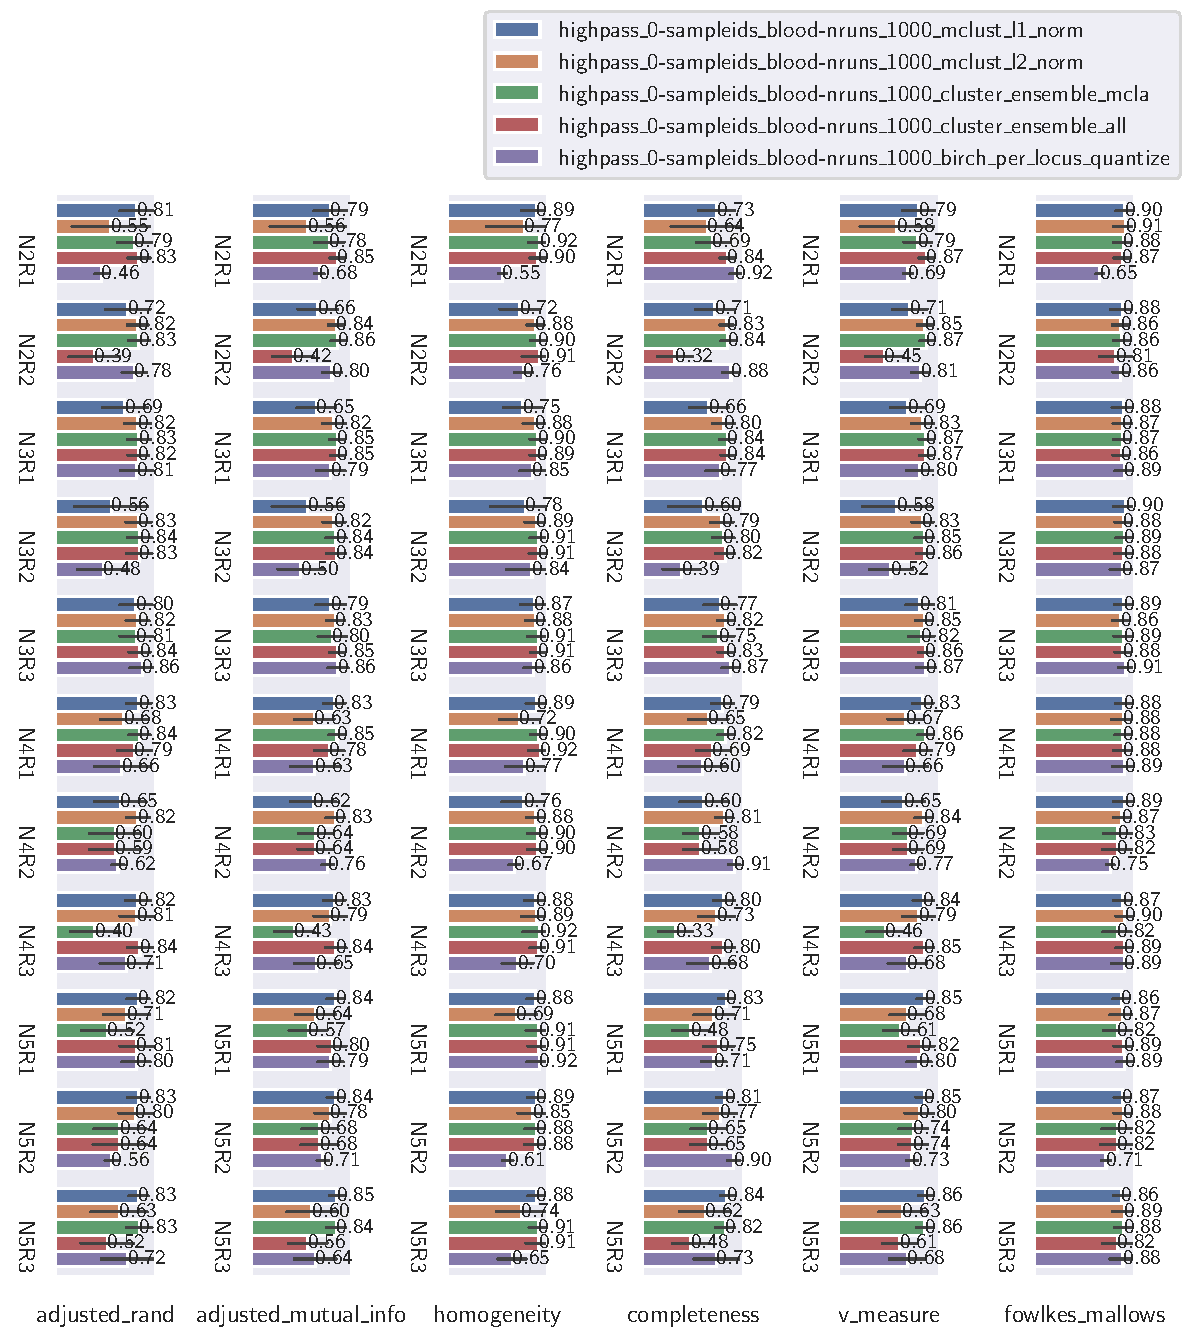
\includegraphics[width=\textwidth]{./figures/clust_comparison/highpass_0-sampleids_blood-nruns_1000_top_5_clusterers_including_ensembles_by_metrics.pdf}
\caption{Top 5 clusterers, including ensembles, clustering performance metrics using 1000 trials sampled from EPGs from only blood samples without high-pass filtering}
\label{fig:highpass_0-sampleids_blood-nruns_1000_top_5_clusterers_including_ensembles_by_metrics}
\end{figure}

\begin{table}[H]
\centering
\maxsizebox{\textwidth}{0.65\textwidth}{
\begin{tabular}{lrr}
\toprule
{} &  mean &    std \\
clusterer                                          &       &        \\
\midrule
mclust\_l2\_norm                                     & 9.10\% & 10.15\% \\
mclust\_l1\_norm                                     & 8.92\% &  9.30\% \\
hdbscan\_euclidean\_epsilon\_0.0\_eom\_per\_locus\_qua... & 4.98\% &  7.95\% \\
hdbscan\_euclidean\_epsilon\_0.5\_eom\_per\_locus\_norm   & 4.90\% &  7.89\% \\
hdbscan\_euclidean\_epsilon\_0.0\_eom\_per\_locus\_norm   & 4.90\% &  7.89\% \\
hdbscan\_euclidean\_epsilon\_1.0\_eom\_per\_locus\_norm   & 4.90\% &  7.89\% \\
affinity\_per\_locus\_quantize                        & 3.75\% &  4.93\% \\
affinity\_per\_locus\_norm                            & 3.61\% &  5.16\% \\
birch\_per\_locus\_norm                               & 3.39\% &  5.53\% \\
birch\_per\_locus\_quantize                           & 3.35\% &  5.47\% \\
birch\_l2\_norm                                      & 3.07\% &  3.95\% \\
cluster\_ensemble\_mcla                              & 3.02\% &  3.20\% \\
cluster\_ensemble\_all                               & 3.01\% &  3.21\% \\
hdbscan\_euclidean\_epsilon\_0.0\_leaf\_per\_locus\_qu... & 2.49\% &  4.09\% \\
meanshift\_per\_locus\_norm                           & 2.10\% &  1.82\% \\
hdbscan\_euclidean\_epsilon\_0.0\_leaf\_per\_locus\_norm  & 1.99\% &  3.50\% \\
hdbscan\_euclidean\_epsilon\_0.5\_leaf\_per\_locus\_norm  & 1.99\% &  3.50\% \\
hdbscan\_euclidean\_epsilon\_1.0\_leaf\_per\_locus\_norm  & 1.99\% &  3.50\% \\
hdbscan\_euclidean\_epsilon\_0.0\_eom\_l2\_norm          & 1.75\% &  2.73\% \\
hdbscan\_euclidean\_epsilon\_0.5\_eom\_l2\_norm          & 1.75\% &  2.73\% \\
hdbscan\_cosine\_epsilon\_0.0\_eom                     & 1.75\% &  2.73\% \\
hdbscan\_euclidean\_epsilon\_0.5\_leaf\_l2\_norm         & 1.72\% &  2.70\% \\
affinity\_l2\_norm                                   & 1.72\% &  2.81\% \\
hdbscan\_euclidean\_epsilon\_0.0\_eom\_l1\_norm          & 1.68\% &  2.32\% \\
optics\_per\_locus\_quantize                          & 1.67\% &  2.79\% \\
\bottomrule
\end{tabular}


}
\caption{Top 25 clusterers by arithmetic mean of percentages of perfect clustering, using admixtures sampled from only blood EPG data without highpass filter}
\label{table:top_25_clusterers_by_binomial_confidence_highpass_0-sampleids_blood-nruns_1000}
\end{table}

\begin{table}[H]
\centering
\maxsizebox{\textwidth}{0.65\textwidth}{
\begin{tabular}{llrrrrrrrrrr}
\toprule
     & {} & \multicolumn{5}{l}{homogeneity} & \multicolumn{5}{l}{completeness} \\
     & clusterer &           1 &      2 &      3 &      4 &      5 &            1 &      2 &      3 &      4 &      5 \\
\midrule
N2R1 & ci\_upp &      69.84\% & 40.95\% &  0.38\% &  4.37\% & 48.00\% &       50.30\% & 21.44\% & 23.22\% &  1.83\% & 29.01\% \\
     & success &      67.00\% & 37.90\% &  0.00\% &  3.10\% & 44.90\% &       47.20\% & 18.90\% & 20.60\% &  1.00\% & 26.20\% \\
     & ci\_low &      64.03\% & 34.94\% &  0.00\% &  2.19\% & 41.84\% &       44.12\% & 16.59\% & 18.21\% &  0.54\% & 23.57\% \\
N2R2 & ci\_upp &       1.02\% & 16.61\% &  2.21\% & 33.53\% & 15.01\% &        0.73\% & 16.08\% & 26.95\% & 23.94\% &  7.65\% \\
     & success &       0.40\% & 14.30\% &  1.30\% & 30.60\% & 12.80\% &        0.20\% & 13.80\% & 24.20\% & 21.30\% &  6.00\% \\
     & ci\_low &       0.16\% & 12.27\% &  0.76\% & 27.82\% & 10.87\% &        0.05\% & 11.80\% & 21.65\% & 18.87\% &  4.69\% \\
N3R1 & ci\_upp &       8.64\% & 23.53\% & 12.12\% &  1.44\% & 12.23\% &        4.83\% & 13.41\% &  7.54\% &  0.56\% &  7.54\% \\
     & success &       6.90\% & 20.90\% & 10.10\% &  0.70\% & 10.20\% &        3.50\% & 11.30\% &  5.90\% &  0.10\% &  5.90\% \\
     & ci\_low &       5.49\% & 18.49\% &  8.38\% &  0.34\% &  8.47\% &        2.53\% &  9.48\% &  4.60\% &  0.02\% &  4.60\% \\
N3R2 & ci\_upp &      10.61\% & 67.01\% & 48.30\% & 22.49\% & 33.53\% &        6.64\% & 44.38\% & 29.42\% & 18.61\% & 23.94\% \\
     & success &       8.70\% & 64.10\% & 45.20\% & 19.90\% & 30.60\% &        5.10\% & 41.30\% & 26.60\% & 16.20\% & 21.30\% \\
     & ci\_low &       7.11\% & 61.08\% & 42.14\% & 17.54\% & 27.82\% &        3.90\% & 38.29\% & 23.95\% & 14.05\% & 18.87\% \\
N3R3 & ci\_upp &       2.95\% & 29.84\% &  5.29\% &  0.56\% &  0.56\% &        1.83\% & 20.08\% &  2.34\% & 19.24\% & 19.24\% \\
     & success &       1.90\% & 27.00\% &  3.90\% &  0.10\% &  0.10\% &        1.00\% & 17.60\% &  1.40\% & 16.80\% & 16.80\% \\
     & ci\_low &       1.22\% & 24.34\% &  2.87\% &  0.02\% &  0.02\% &        0.54\% & 15.36\% &  0.84\% & 14.61\% & 14.61\% \\
N4R1 & ci\_upp &      20.19\% & 11.26\% & 14.91\% & 12.23\% &  0.38\% &       12.45\% &  6.19\% &  7.98\% &  7.54\% & 18.82\% \\
     & success &      17.70\% &  9.30\% & 12.70\% & 10.20\% &  0.00\% &       10.40\% &  4.70\% &  6.30\% &  5.90\% & 16.40\% \\
     & ci\_low &      15.46\% &  7.65\% & 10.78\% &  8.47\% &  0.00\% &        8.66\% &  3.55\% &  4.95\% &  4.60\% & 14.23\% \\
N4R2 & ci\_upp &       3.78\% & 35.67\% &  4.25\% &  0.38\% &  4.37\% &        2.46\% & 19.56\% &  1.96\% & 18.82\% &  1.83\% \\
     & success &       2.60\% & 32.70\% &  3.00\% &  0.00\% &  3.10\% &        1.50\% & 17.10\% &  1.10\% & 16.40\% &  1.00\% \\
     & ci\_low &       1.78\% & 29.86\% &  2.11\% &  0.00\% &  2.19\% &        0.91\% & 14.89\% &  0.62\% & 14.23\% &  0.54\% \\
N4R3 & ci\_upp &      41.35\% &  9.19\% & 33.01\% & 48.00\% &  5.74\% &       22.49\% &  4.83\% & 31.17\% & 29.01\% &  2.58\% \\
     & success &      38.30\% &  7.40\% & 30.10\% & 44.90\% &  4.30\% &       19.90\% &  3.50\% & 28.30\% & 26.20\% &  1.60\% \\
     & ci\_low &      35.34\% &  5.94\% & 27.34\% & 41.84\% &  3.21\% &       17.54\% &  2.53\% & 25.60\% & 23.57\% &  0.99\% \\
N5R1 & ci\_upp &      13.95\% &  3.31\% &  1.70\% &  0.38\% &  0.38\% &       16.82\% &  1.83\% &  0.38\% & 18.19\% & 18.19\% \\
     & success &      11.80\% &  2.20\% &  0.90\% &  0.00\% &  0.00\% &       14.50\% &  1.00\% &  0.00\% & 15.80\% & 15.80\% \\
     & ci\_low &       9.95\% &  1.46\% &  0.47\% &  0.00\% &  0.00\% &       12.45\% &  0.54\% &  0.00\% & 13.67\% & 13.67\% \\
N5R2 & ci\_upp &      29.12\% &  3.66\% &  0.38\% &  5.74\% & 22.49\% &       20.92\% &  1.83\% & 22.28\% &  2.58\% & 18.61\% \\
     & success &      26.30\% &  2.50\% &  0.00\% &  4.30\% & 19.90\% &       18.40\% &  1.00\% & 19.70\% &  1.60\% & 16.20\% \\
     & ci\_low &      23.67\% &  1.70\% &  0.00\% &  3.21\% & 17.54\% &       16.12\% &  0.54\% & 17.35\% &  0.99\% & 14.05\% \\
N5R3 & ci\_upp &      35.57\% &  1.30\% & 22.70\% & 15.01\% &  1.44\% &       22.49\% &  0.73\% & 18.19\% &  7.65\% &  0.56\% \\
     & success &      32.60\% &  0.60\% & 20.10\% & 12.80\% &  0.70\% &       19.90\% &  0.20\% & 15.80\% &  6.00\% &  0.10\% \\
     & ci\_low &      29.77\% &  0.28\% & 17.73\% & 10.87\% &  0.34\% &       17.54\% &  0.05\% & 13.67\% &  4.69\% &  0.02\% \\
\bottomrule
\end{tabular}


}
\caption{Top 5 clusterers, including ensembles, clustering percentages of trials where no error occurs using 1000 trials sampled from EPGs from only blood samples without high-pass filtering}
\label{table:highpass_0-sampleids_blood-nruns_1000_top_5_clusterers_including_ensembles_by_binomial_confidence}
\end{table}

\subsection{Blood Samples Only, with High-Pass Filtering}

\begin{table}[H]
\centering
\maxsizebox{\textwidth}{0.65\textwidth}{
\begin{tabular}{lrr}
\toprule
{} &      mean &       std \\
clusterer                                          &           &           \\
\midrule
mclust\_l1\_norm                                     &  0.960895 &  0.098183 \\
mclust\_l2\_norm                                     &  0.953501 &  0.107068 \\
cluster\_ensemble\_mcla                              &  0.906558 &  0.168099 \\
cluster\_ensemble\_all                               &  0.900609 &  0.183406 \\
birch\_per\_locus\_quantize                           &  0.849550 &  0.173975 \\
affinity\_per\_locus\_quantize                        &  0.844791 &  0.250112 \\
birch\_per\_locus\_norm                               &  0.842968 &  0.184070 \\
affinity\_per\_locus\_norm                            &  0.792776 &  0.294350 \\
affinity\_l1\_norm                                   &  0.791961 &  0.290986 \\
affinity\_l2\_norm                                   &  0.787894 &  0.297917 \\
birch\_l2\_norm                                      &  0.779446 &  0.227425 \\
hdbscan\_euclidean\_epsilon\_0.0\_eom\_per\_locus\_qua... &  0.777033 &  0.348583 \\
meanshift\_per\_locus\_norm                           &  0.768090 &  0.356926 \\
hdbscan\_euclidean\_epsilon\_0.5\_eom\_l2\_norm          &  0.767799 &  0.354855 \\
hdbscan\_euclidean\_epsilon\_0.0\_eom\_l2\_norm          &  0.767208 &  0.356015 \\
hdbscan\_euclidean\_epsilon\_0.5\_leaf\_l2\_norm         &  0.765516 &  0.354534 \\
meanshift\_l2\_norm                                  &  0.765354 &  0.356738 \\
hdbscan\_cosine\_epsilon\_0.0\_eom                     &  0.764884 &  0.356171 \\
hdbscan\_euclidean\_epsilon\_0.0\_eom\_l1\_norm          &  0.763600 &  0.359556 \\
hdbscan\_cosine\_epsilon\_0.0\_eom\_per\_locus\_norm      &  0.759901 &  0.362087 \\
hdbscan\_euclidean\_epsilon\_0.0\_eom\_per\_locus\_norm   &  0.757295 &  0.366148 \\
hdbscan\_euclidean\_epsilon\_1.0\_eom\_per\_locus\_norm   &  0.757295 &  0.366148 \\
hdbscan\_euclidean\_epsilon\_0.5\_eom\_per\_locus\_norm   &  0.757295 &  0.366148 \\
meanshift\_l1\_norm                                  &  0.754057 &  0.354813 \\
meanshift\_per\_locus\_quantize                       &  0.748134 &  0.354944 \\
\bottomrule
\end{tabular}


}
\caption{Top 25 clusterers, including ensembles, by arithmetic mean of clustering metric scores, using admixtures sampled from only blood EPG data with highpass filter}
\label{table:top_25_clusterers_by_metrics_highpass_71-sampleids_blood-nruns_1000}
\end{table}

\begin{figure}[H]
\centering
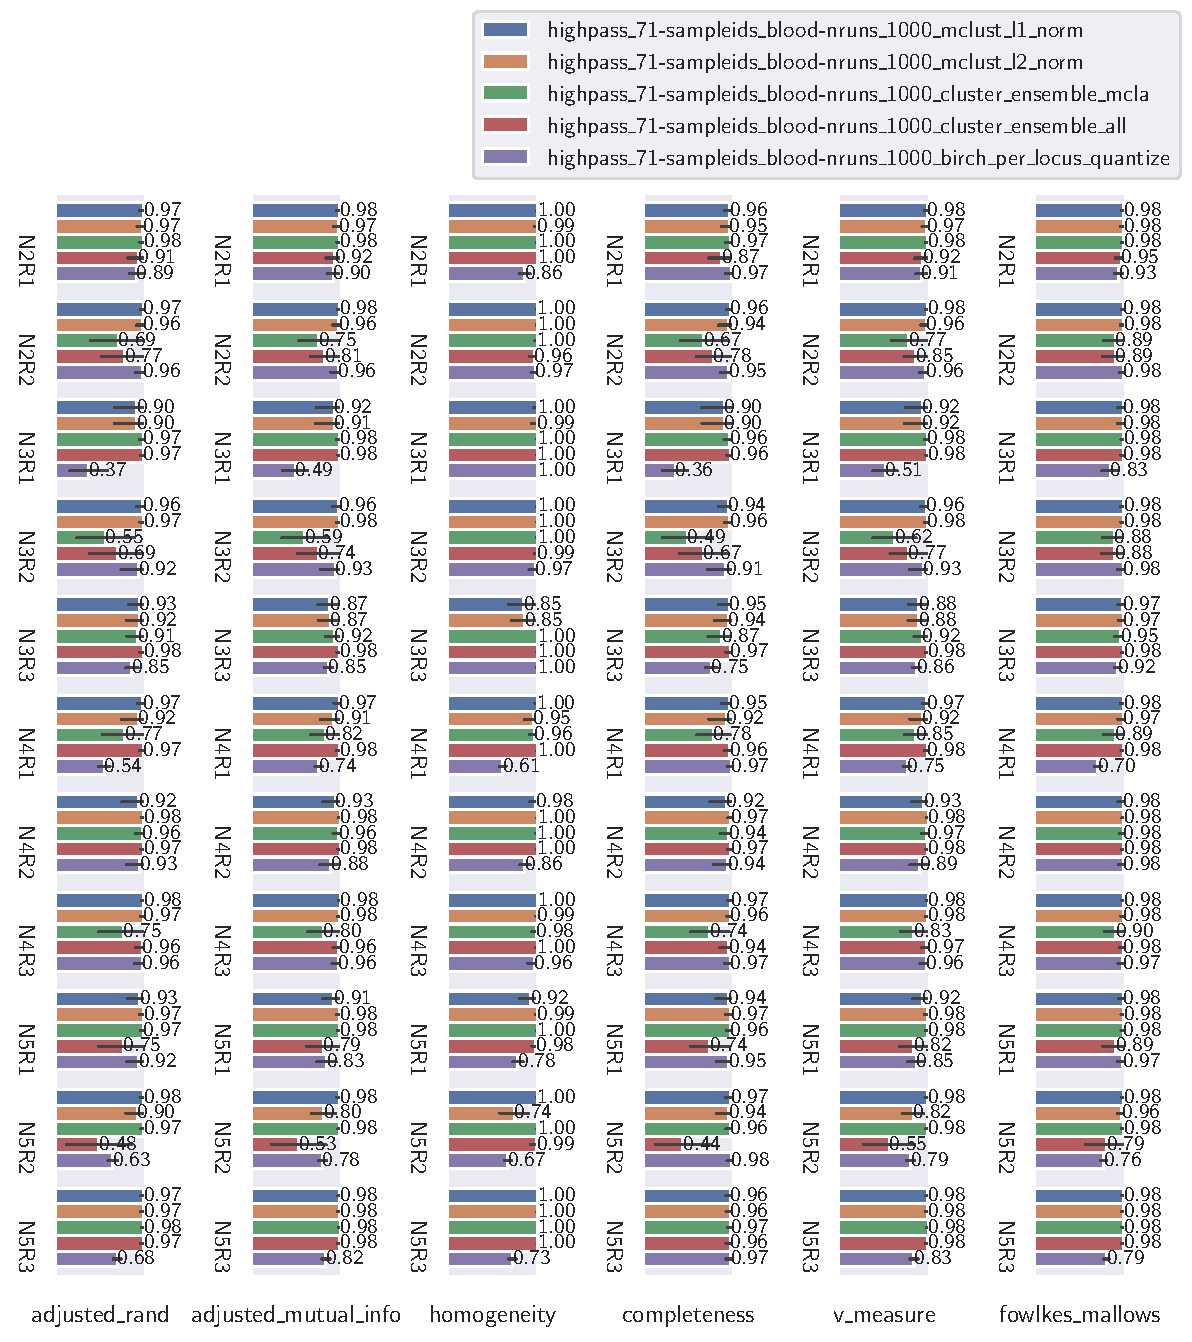
\includegraphics[width=\textwidth]{./figures/clust_comparison/highpass_71-sampleids_blood-nruns_1000_top_5_clusterers_including_ensembles_by_metrics.pdf}
\caption{Top 5 clusterers, including ensembles, clustering performance metrics using 1000 trials sampled from EPGs from only blood samples with high-pass filtering}
\label{fig:highpass_71-sampleids_blood-nruns_1000_top_5_clusterers_including_ensembles_by_metrics}
\end{figure}

\begin{table}[H]
\centering
\maxsizebox{\textwidth}{0.65\textwidth}{
\begin{tabular}{lrr}
\toprule
{} &   mean &    std \\
clusterer                                          &        &        \\
\midrule
mclust\_l1\_norm                                     & 64.13\% & 12.62\% \\
mclust\_l2\_norm                                     & 59.02\% & 18.32\% \\
cluster\_ensemble\_mcla                              & 42.46\% & 22.34\% \\
cluster\_ensemble\_all                               & 42.43\% & 22.43\% \\
affinity\_per\_locus\_quantize                        & 39.18\% & 29.74\% \\
affinity\_per\_locus\_norm                            & 39.05\% & 30.77\% \\
affinity\_l1\_norm                                   & 38.79\% & 30.49\% \\
affinity\_l2\_norm                                   & 38.67\% & 30.44\% \\
hdbscan\_euclidean\_epsilon\_0.0\_eom\_per\_locus\_norm   & 36.66\% & 29.52\% \\
hdbscan\_euclidean\_epsilon\_0.5\_eom\_per\_locus\_norm   & 36.66\% & 29.52\% \\
hdbscan\_euclidean\_epsilon\_1.0\_eom\_per\_locus\_norm   & 36.66\% & 29.52\% \\
hdbscan\_cosine\_epsilon\_0.0\_eom\_per\_locus\_norm      & 36.57\% & 29.50\% \\
hdbscan\_euclidean\_epsilon\_0.0\_eom\_per\_locus\_qua... & 36.15\% & 29.37\% \\
hdbscan\_euclidean\_epsilon\_0.0\_eom\_l2\_norm          & 36.15\% & 29.42\% \\
hdbscan\_euclidean\_epsilon\_0.5\_eom\_l2\_norm          & 36.15\% & 29.42\% \\
hdbscan\_cosine\_epsilon\_0.0\_eom                     & 36.15\% & 29.42\% \\
hdbscan\_euclidean\_epsilon\_0.0\_eom\_l1\_norm          & 36.06\% & 29.25\% \\
hdbscan\_euclidean\_epsilon\_0.5\_leaf\_l2\_norm         & 35.25\% & 28.76\% \\
hdbscan\_cosine\_epsilon\_0.0\_eom\_per\_locus\_quantize  & 30.66\% & 25.33\% \\
meanshift\_per\_locus\_norm                           & 30.12\% & 21.63\% \\
meanshift\_l2\_norm                                  & 28.52\% & 21.48\% \\
hdbscan\_cosine\_epsilon\_0.5\_eom\_per\_locus\_norm      & 26.82\% & 24.40\% \\
hdbscan\_cosine\_epsilon\_0.5\_leaf\_per\_locus\_norm     & 26.82\% & 24.40\% \\
birch\_l2\_norm                                      & 23.59\% & 28.61\% \\
meanshift\_l1\_norm                                  & 22.28\% & 18.21\% \\
\bottomrule
\end{tabular}


}
\caption{Top 25 clusterers by arithmetic mean of percentages of perfect clustering, using admixtures sampled from only blood EPG data with highpass filter}
\label{table:top_25_clusterers_by_binomial_confidence_highpass_71-sampleids_blood-nruns_1000}
\end{table}

\begin{table}[H]
\centering
\maxsizebox{\textwidth}{0.65\textwidth}{
\begin{tabular}{llrrrrrrrrrr}
\toprule
     & {} & \multicolumn{5}{l}{homogeneity} & \multicolumn{5}{l}{completeness} \\
     & clusterer &           1 &      2 &      3 &      4 &      5 &            1 &      2 &      3 &      4 &      5 \\
\midrule
N2R1 & ci\_upp &      98.62\% & 94.69\% & 97.72\% & 99.95\% & 95.93\% &       70.33\% & 78.74\% & 68.97\% & 54.69\% & 68.38\% \\
     & success &      97.90\% & 93.30\% & 96.80\% & 99.80\% & 94.70\% &       67.50\% & 76.20\% & 66.10\% & 51.60\% & 65.50\% \\
     & ci\_low &      96.81\% & 91.58\% & 95.52\% & 99.27\% & 93.13\% &       64.53\% & 73.46\% & 63.11\% & 48.50\% & 62.50\% \\
N2R2 & ci\_upp &      92.17\% & 99.24\% & 98.30\% & 63.19\% & 99.66\% &       55.58\% & 78.45\% & 21.76\% & 17.03\% & 74.50\% \\
     & success &      90.50\% & 98.70\% & 97.50\% & 60.20\% & 99.30\% &       52.50\% & 75.90\% & 19.20\% & 14.70\% & 71.80\% \\
     & ci\_low &      88.52\% & 97.79\% & 96.34\% & 57.13\% & 98.56\% &       49.40\% & 73.15\% & 16.88\% & 12.64\% & 68.93\% \\
N3R1 & ci\_upp &      99.90\% & 99.66\% & 98.70\% & 91.80\% & 97.39\% &       86.61\% & 86.80\% & 69.36\% & 53.49\% & 57.37\% \\
     & success &      99.70\% & 99.30\% & 98.00\% & 90.10\% & 96.40\% &       84.50\% & 84.70\% & 66.50\% & 50.40\% & 54.30\% \\
     & ci\_low &      99.12\% & 98.56\% & 96.93\% & 88.09\% & 95.06\% &       82.13\% & 82.34\% & 63.52\% & 47.31\% & 51.20\% \\
N3R2 & ci\_upp &      99.16\% & 98.62\% & 99.95\% & 97.39\% & 97.39\% &       78.35\% & 70.62\% & 15.33\% & 21.76\% & 51.60\% \\
     & success &      98.60\% & 97.90\% & 99.80\% & 96.40\% & 96.40\% &       75.80\% & 67.80\% & 13.10\% & 19.20\% & 48.50\% \\
     & ci\_low &      97.66\% & 96.81\% & 99.27\% & 95.06\% & 95.06\% &       73.05\% & 64.84\% & 11.15\% & 16.88\% & 45.41\% \\
N3R3 & ci\_upp &      54.49\% & 48.10\% & 99.95\% & 97.81\% & 98.54\% &       86.61\% & 87.83\% & 54.39\% & 69.16\% & 68.77\% \\
     & success &      51.40\% & 45.00\% & 99.80\% & 96.90\% & 97.80\% &       84.50\% & 85.80\% & 51.30\% & 66.30\% & 65.90\% \\
     & ci\_low &      48.30\% & 41.94\% & 99.27\% & 95.63\% & 96.69\% &       82.13\% & 83.50\% & 48.20\% & 63.31\% & 62.91\% \\
N4R1 & ci\_upp &      96.45\% & 77.68\% & 63.48\% & 98.70\% & 91.07\% &       78.45\% & 86.42\% & 17.03\% & 69.36\% &  7.54\% \\
     & success &      95.30\% & 75.10\% & 60.50\% & 98.00\% & 89.30\% &       75.90\% & 84.30\% & 14.70\% & 66.50\% &  5.90\% \\
     & ci\_low &      93.81\% & 72.33\% & 57.44\% & 96.93\% & 87.23\% &       73.15\% & 81.91\% & 12.64\% & 63.52\% &  4.60\% \\
N4R2 & ci\_upp &      89.13\% & 95.05\% & 97.64\% & 94.24\% & 95.13\% &       86.42\% & 53.39\% & 72.37\% & 51.70\% & 74.98\% \\
     & success &      87.20\% & 93.70\% & 96.70\% & 92.80\% & 93.80\% &       84.30\% & 50.30\% & 69.60\% & 48.60\% & 72.30\% \\
     & ci\_low &      84.99\% & 92.02\% & 95.40\% & 91.03\% & 92.13\% &       81.91\% & 47.21\% & 66.68\% & 45.51\% & 69.44\% \\
N4R3 & ci\_upp &      96.88\% & 87.73\% & 83.50\% & 97.64\% & 92.44\% &       53.29\% & 55.48\% & 18.09\% & 72.47\% & 52.00\% \\
     & success &      95.80\% & 85.70\% & 81.20\% & 96.70\% & 90.80\% &       50.20\% & 52.40\% & 15.70\% & 69.70\% & 48.90\% \\
     & ci\_low &      94.37\% & 83.39\% & 78.66\% & 95.40\% & 88.85\% &       47.11\% & 49.30\% & 13.58\% & 66.78\% & 45.81\% \\
N5R1 & ci\_upp &      71.89\% & 92.35\% & 91.89\% & 82.84\% & 83.31\% &       87.64\% & 71.60\% & 53.29\% & 18.09\% & 14.59\% \\
     & success &      69.10\% & 90.70\% & 90.20\% & 80.50\% & 81.00\% &       85.60\% & 68.80\% & 50.20\% & 15.70\% & 12.40\% \\
     & ci\_low &      66.17\% & 88.74\% & 88.20\% & 77.93\% & 78.45\% &       83.29\% & 65.86\% & 47.11\% & 13.58\% & 10.50\% \\
N5R2 & ci\_upp &      95.66\% & 25.71\% & 97.47\% & 96.88\% & 96.36\% &       71.89\% & 86.80\% & 57.96\% & 14.80\% &  5.51\% \\
     & success &      94.40\% & 23.00\% & 96.50\% & 95.80\% & 95.20\% &       69.10\% & 84.70\% & 54.90\% & 12.60\% &  4.10\% \\
     & ci\_low &      92.80\% & 20.50\% & 95.17\% & 94.37\% & 93.69\% &       66.17\% & 82.34\% & 51.80\% & 10.69\% &  3.04\% \\
N5R3 & ci\_upp &      97.30\% & 96.19\% & 97.22\% & 97.47\% & 86.89\% &       59.05\% & 59.05\% & 52.10\% & 57.86\% &  9.19\% \\
     & success &      96.30\% & 95.00\% & 96.20\% & 96.50\% & 84.80\% &       56.00\% & 56.00\% & 49.00\% & 54.80\% &  7.40\% \\
     & ci\_low &      94.94\% & 93.47\% & 94.83\% & 95.17\% & 82.44\% &       52.91\% & 52.91\% & 45.91\% & 51.70\% &  5.94\% \\
\bottomrule
\end{tabular}


}
\caption{Top 5 clusterers, including ensembles, clustering percentages of trials where no error occurs using 1000 trials sampled from EPGs from only blood samples with high-pass filtering}
\label{table:highpass_71-sampleids_blood-nruns_1000_top_5_clusterers_including_ensembles_by_binomial_confidence}
\end{table}

\subsection{All Samples, without High-Pass Filtering}

\begin{table}[H]
\centering
\maxsizebox{\textwidth}{0.65\textwidth}{
\begin{tabular}{lrr}
\toprule
{} &      mean &       std \\
clusterer                                          &           &           \\
\midrule
birch\_per\_locus\_quantize                           &  0.641797 &  0.211116 \\
birch\_per\_locus\_norm                               &  0.641290 &  0.211306 \\
cluster\_ensemble\_mcla                              &  0.639000 &  0.209602 \\
cluster\_ensemble\_all                               &  0.637556 &  0.212475 \\
mclust\_l1\_norm                                     &  0.632317 &  0.234902 \\
mclust\_l2\_norm                                     &  0.628675 &  0.240790 \\
affinity\_per\_locus\_quantize                        &  0.626572 &  0.227781 \\
affinity\_l2\_norm                                   &  0.616125 &  0.234093 \\
hdbscan\_euclidean\_epsilon\_0.0\_eom\_per\_locus\_qua... &  0.606724 &  0.259711 \\
hdbscan\_euclidean\_epsilon\_0.5\_eom\_per\_locus\_norm   &  0.606178 &  0.262164 \\
hdbscan\_euclidean\_epsilon\_0.0\_eom\_per\_locus\_norm   &  0.606178 &  0.262164 \\
hdbscan\_euclidean\_epsilon\_1.0\_eom\_per\_locus\_norm   &  0.606178 &  0.262164 \\
affinity\_per\_locus\_norm                            &  0.601773 &  0.234468 \\
meanshift\_per\_locus\_norm                           &  0.588258 &  0.305518 \\
meanshift\_per\_locus\_quantize                       &  0.583719 &  0.298994 \\
hdbscan\_cosine\_epsilon\_0.0\_eom\_per\_locus\_norm      &  0.579221 &  0.314593 \\
hdbscan\_euclidean\_epsilon\_0.5\_eom\_l2\_norm          &  0.576326 &  0.308595 \\
hdbscan\_euclidean\_epsilon\_0.0\_eom\_l2\_norm          &  0.575876 &  0.309118 \\
hdbscan\_cosine\_epsilon\_0.0\_eom                     &  0.569691 &  0.308828 \\
hdbscan\_cosine\_epsilon\_0.0\_eom\_per\_locus\_quantize  &  0.567093 &  0.303365 \\
hdbscan\_euclidean\_epsilon\_0.5\_leaf\_l2\_norm         &  0.563626 &  0.308553 \\
hdbscan\_cosine\_epsilon\_0.5\_eom\_per\_locus\_norm      &  0.562861 &  0.307425 \\
hdbscan\_cosine\_epsilon\_0.5\_leaf\_per\_locus\_norm     &  0.562268 &  0.305130 \\
affinity\_l1\_norm                                   &  0.561750 &  0.265127 \\
hdbscan\_euclidean\_epsilon\_0.0\_eom\_l1\_norm          &  0.536147 &  0.311479 \\
\bottomrule
\end{tabular}


}
\caption{Top 25 clusterers, including ensembles, by arithmetic mean of clustering metric scores, using admixtures sampled from all EPG data without highpass filter}
\label{table:top_25_clusterers_by_metrics_highpass_0-sampleids_all-nruns_1000}
\end{table}

\begin{figure}[H]
\centering
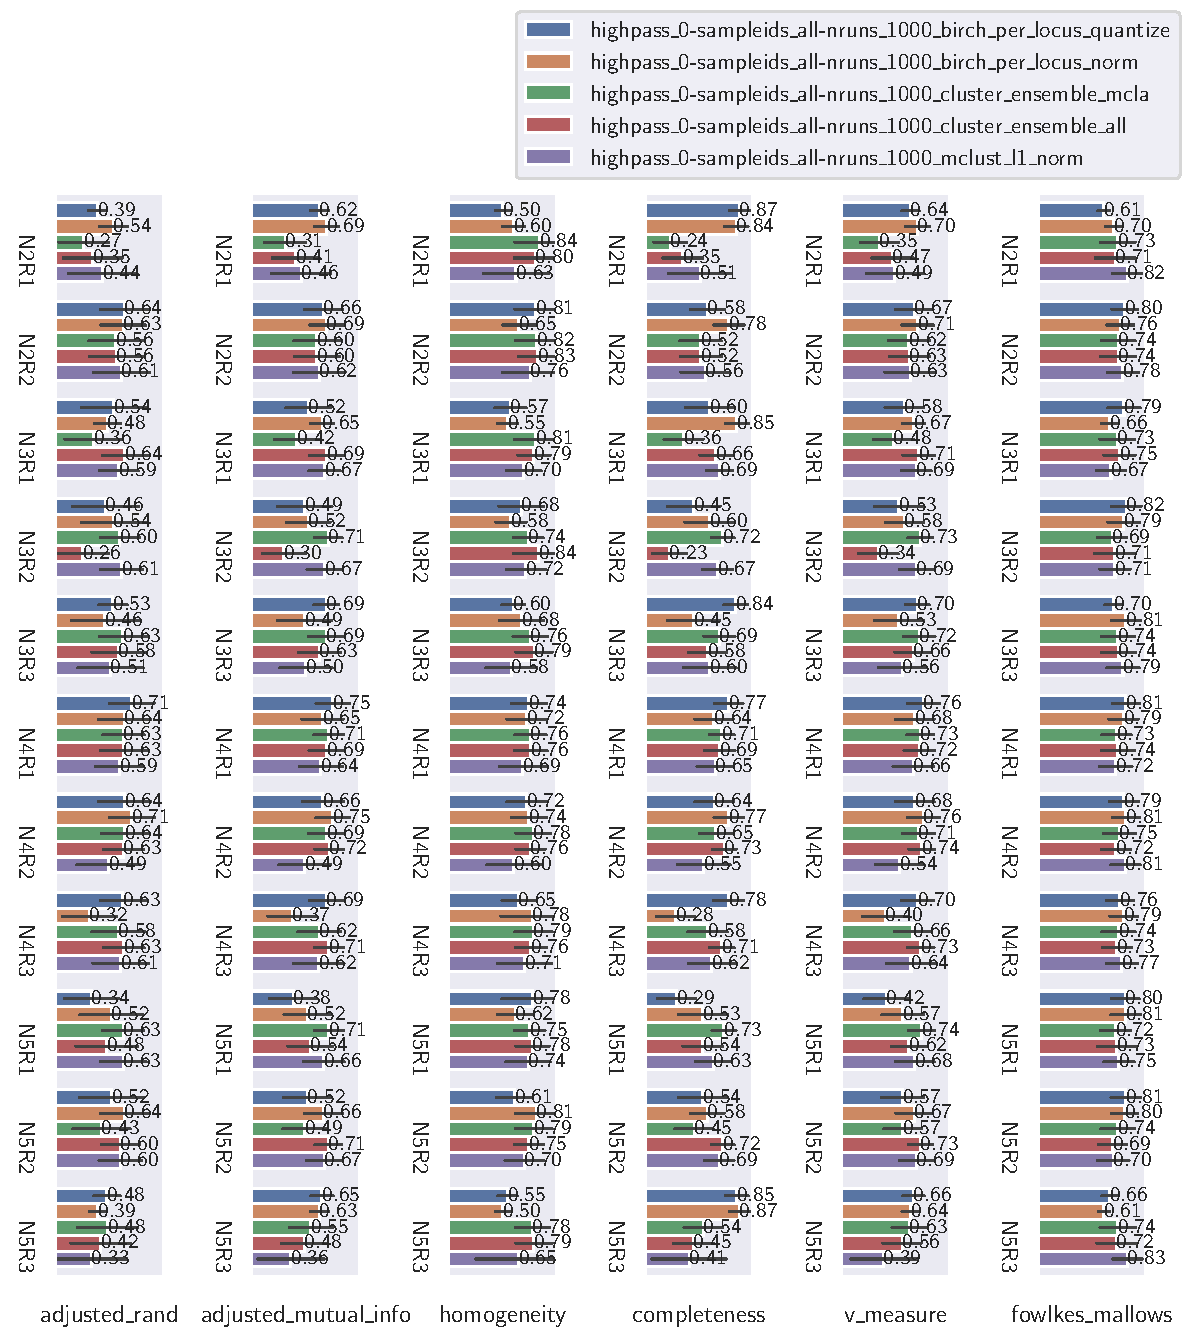
\includegraphics[width=\textwidth]{./figures/clust_comparison/highpass_0-sampleids_all-nruns_1000_top_5_clusterers_including_ensembles_by_metrics.pdf}
\caption{Top 5 clusterers, including ensembles, clustering performance metrics using 1000 trials sampled from all EPGs without high-pass filtering}
\label{fig:highpass_0-sampleids_all-nruns_1000_top_5_clusterers_including_ensembles_by_metrics}
\end{figure}

\begin{table}[H]
\centering
\maxsizebox{\textwidth}{0.65\textwidth}{
\begin{tabular}{lrr}
\toprule
{} &  mean &   std \\
clusterer                                          &       &       \\
\midrule
mclust\_l2\_norm                                     & 3.09\% & 4.12\% \\
mclust\_l1\_norm                                     & 2.97\% & 3.75\% \\
meanshift\_per\_locus\_norm                           & 2.66\% & 2.49\% \\
hdbscan\_euclidean\_epsilon\_1.0\_eom\_per\_locus\_norm   & 2.39\% & 4.63\% \\
hdbscan\_euclidean\_epsilon\_0.0\_eom\_per\_locus\_norm   & 2.39\% & 4.63\% \\
hdbscan\_euclidean\_epsilon\_0.5\_eom\_per\_locus\_norm   & 2.39\% & 4.63\% \\
hdbscan\_euclidean\_epsilon\_0.0\_eom\_per\_locus\_qua... & 2.23\% & 4.47\% \\
meanshift\_per\_locus\_quantize                       & 1.91\% & 1.98\% \\
birch\_per\_locus\_quantize                           & 1.78\% & 2.88\% \\
birch\_per\_locus\_norm                               & 1.73\% & 2.79\% \\
birch\_l2\_norm                                      & 1.25\% & 1.63\% \\
affinity\_per\_locus\_norm                            & 1.22\% & 2.13\% \\
affinity\_per\_locus\_quantize                        & 1.18\% & 1.97\% \\
optics\_per\_locus\_quantize                          & 1.18\% & 2.40\% \\
optics\_per\_locus\_norm                              & 1.14\% & 2.16\% \\
hdbscan\_euclidean\_epsilon\_0.0\_leaf\_per\_locus\_qu... & 0.99\% & 2.03\% \\
hdbscan\_euclidean\_epsilon\_1.0\_leaf\_per\_locus\_norm  & 0.95\% & 1.79\% \\
hdbscan\_euclidean\_epsilon\_0.0\_leaf\_per\_locus\_norm  & 0.95\% & 1.79\% \\
hdbscan\_euclidean\_epsilon\_0.5\_leaf\_per\_locus\_norm  & 0.95\% & 1.79\% \\
hdbscan\_euclidean\_epsilon\_0.0\_eom\_l2\_norm          & 0.81\% & 1.41\% \\
hdbscan\_euclidean\_epsilon\_0.5\_eom\_l2\_norm          & 0.81\% & 1.41\% \\
cluster\_ensemble\_all                               & 0.80\% & 1.05\% \\
hdbscan\_cosine\_epsilon\_0.0\_eom                     & 0.80\% & 1.38\% \\
cluster\_ensemble\_mcla                              & 0.79\% & 1.04\% \\
hdbscan\_euclidean\_epsilon\_0.5\_leaf\_l2\_norm         & 0.74\% & 1.27\% \\
\bottomrule
\end{tabular}


}
\caption{Top 25 clusterers by arithmetic mean of percentages of perfect clustering, using admixtures sampled from all EPG data without highpass filter}
\label{table:top_25_clusterers_by_binomial_confidence_highpass_0-sampleids_all-nruns_1000}
\end{table}

\begin{table}[H]
\centering
\maxsizebox{\textwidth}{0.65\textwidth}{
\begin{tabular}{llrrrrrrrrrr}
\toprule
     & {} & \multicolumn{5}{l}{homogeneity} & \multicolumn{5}{l}{completeness} \\
     & clusterer &           1 &      2 &      3 &      4 &      5 &            1 &      2 &      3 &      4 &      5 \\
\midrule
N2R1 & ci\_upp &       2.46\% & 23.63\% & 21.23\% &  3.66\% &  0.88\% &        1.57\% & 19.66\% &  8.86\% &  4.71\% &  1.44\% \\
     & success &       1.50\% & 21.00\% & 18.70\% &  2.50\% &  0.30\% &        0.80\% & 17.20\% &  7.10\% &  3.40\% &  0.70\% \\
     & ci\_low &       0.91\% & 18.59\% & 16.40\% &  1.70\% &  0.10\% &        0.41\% & 14.99\% &  5.67\% &  2.44\% &  0.34\% \\
N2R2 & ci\_upp &       4.48\% & 27.57\% & 27.16\% &  0.38\% &  6.64\% &        1.57\% &  9.30\% &  7.76\% &  0.38\% &  4.83\% \\
     & success &       3.20\% & 24.80\% & 24.40\% &  0.00\% &  5.10\% &        0.80\% &  7.50\% &  6.10\% &  0.00\% &  3.50\% \\
     & ci\_low &       2.28\% & 22.22\% & 21.84\% &  0.00\% &  3.90\% &        0.41\% &  6.03\% &  4.78\% &  0.00\% &  2.53\% \\
N3R1 & ci\_upp &      22.70\% &  0.38\% &  0.38\% &  1.02\% &  3.66\% &       23.94\% &  0.38\% & 75.18\% &  1.44\% &  4.71\% \\
     & success &      20.10\% &  0.00\% &  0.00\% &  0.40\% &  2.50\% &       21.30\% &  0.00\% & 72.50\% &  0.70\% &  3.40\% \\
     & ci\_low &      17.73\% &  0.00\% &  0.00\% &  0.16\% &  1.70\% &       18.87\% &  0.00\% & 69.65\% &  0.34\% &  2.44\% \\
N3R2 & ci\_upp &       0.73\% &  0.88\% &  0.38\% &  6.64\% &  0.38\% &        0.73\% &  0.73\% & 76.24\% &  4.83\% &  0.38\% \\
     & success &       0.20\% &  0.30\% &  0.00\% &  5.10\% &  0.00\% &        0.20\% &  0.20\% & 73.60\% &  3.50\% &  0.00\% \\
     & ci\_low &       0.05\% &  0.10\% &  0.00\% &  3.90\% &  0.00\% &        0.05\% &  0.05\% & 70.78\% &  2.53\% &  0.00\% \\
N3R3 & ci\_upp &       0.38\% &  5.17\% & 17.45\% & 11.04\% &  0.38\% &        0.38\% & 14.27\% &  9.19\% & 12.77\% & 12.02\% \\
     & success &       0.00\% &  3.80\% & 15.10\% &  9.10\% &  0.00\% &        0.00\% & 12.10\% &  7.40\% & 10.70\% & 10.00\% \\
     & ci\_low &       0.00\% &  2.78\% & 13.01\% &  7.47\% &  0.00\% &        0.00\% & 10.22\% &  5.94\% &  8.93\% &  8.29\% \\
N4R1 & ci\_upp &      53.59\% &  2.58\% & 68.09\% &  0.38\% & 11.04\% &       29.73\% &  1.70\% &  9.52\% & 12.98\% & 12.77\% \\
     & success &      50.50\% &  1.60\% & 65.20\% &  0.00\% &  9.10\% &       26.90\% &  0.90\% &  7.70\% & 10.90\% & 10.70\% \\
     & ci\_low &      47.41\% &  0.99\% & 62.19\% &  0.00\% &  7.47\% &       24.24\% &  0.47\% &  6.20\% &  9.12\% &  8.93\% \\
N4R2 & ci\_upp &       8.75\% &  9.08\% & 33.73\% &  0.38\% &  0.38\% &       14.59\% & 11.04\% &  7.65\% & 12.45\% & 12.45\% \\
     & success &       7.00\% &  7.30\% & 30.80\% &  0.00\% &  0.00\% &       12.40\% &  9.10\% &  6.00\% & 10.40\% & 10.40\% \\
     & ci\_low &       5.58\% &  5.85\% & 28.02\% &  0.00\% &  0.00\% &       10.50\% &  7.47\% &  4.69\% &  8.66\% &  8.66\% \\
N4R3 & ci\_upp &       0.73\% & 14.59\% &  7.31\% & 30.56\% & 30.56\% &        0.88\% &  8.64\% & 13.73\% & 20.19\% & 20.19\% \\
     & success &       0.20\% & 12.40\% &  5.70\% & 27.70\% & 27.70\% &        0.30\% &  6.90\% & 11.60\% & 17.70\% & 17.70\% \\
     & ci\_low &       0.05\% & 10.50\% &  4.43\% & 25.02\% & 25.02\% &        0.10\% &  5.49\% &  9.76\% & 15.46\% & 15.46\% \\
N5R1 & ci\_upp &      14.59\% &  5.06\% & 43.27\% &  0.88\% & 19.56\% &       10.28\% &  1.96\% & 12.12\% &  1.44\% & 13.09\% \\
     & success &      12.40\% &  3.70\% & 40.20\% &  0.30\% & 17.10\% &        8.40\% &  1.10\% & 10.10\% &  0.70\% & 11.00\% \\
     & ci\_low &      10.50\% &  2.70\% & 37.20\% &  0.10\% & 14.89\% &        6.84\% &  0.62\% &  8.38\% &  0.34\% &  9.21\% \\
N5R2 & ci\_upp &      27.36\% &  0.56\% &  0.38\% &  0.38\% &  1.02\% &        9.63\% &  0.73\% & 72.95\% & 12.02\% &  1.44\% \\
     & success &      24.60\% &  0.10\% &  0.00\% &  0.00\% &  0.40\% &        7.80\% &  0.20\% & 70.20\% & 10.00\% &  0.70\% \\
     & ci\_low &      22.03\% &  0.02\% &  0.00\% &  0.00\% &  0.16\% &        6.29\% &  0.05\% & 67.29\% &  8.29\% &  0.34\% \\
N5R3 & ci\_upp &       4.25\% & 52.69\% &  4.48\% & 19.56\% &  0.38\% &       16.08\% & 24.78\% & 22.80\% & 13.09\% & 12.98\% \\
     & success &       3.00\% & 49.60\% &  3.20\% & 17.10\% &  0.00\% &       13.80\% & 22.10\% & 20.20\% & 11.00\% & 10.90\% \\
     & ci\_low &       2.11\% & 46.51\% &  2.28\% & 14.89\% &  0.00\% &       11.80\% & 19.64\% & 17.83\% &  9.21\% &  9.12\% \\
\bottomrule
\end{tabular}


}
\caption{Top 5 clusterers, including ensembles, clustering percentages of trials where no error occurs using 1000 trials sampled from all EPGs without high-pass filtering}
\label{table:highpass_0-sampleids_all-nruns_1000_top_5_clusterers_including_ensembles_by_binomial_confidence}
\end{table}

\subsection{All Samples, with High-Pass Filtering}

\begin{table}[H]
\centering
\maxsizebox{\textwidth}{0.65\textwidth}{
\begin{tabular}{lrr}
\toprule
{} &      mean &       std \\
clusterer                                          &           &           \\
\midrule
mclust\_l2\_norm                                     &  0.937051 &  0.136490 \\
mclust\_l1\_norm                                     &  0.936063 &  0.136644 \\
cluster\_ensemble\_mcla                              &  0.879164 &  0.193338 \\
cluster\_ensemble\_all                               &  0.873449 &  0.206286 \\
birch\_per\_locus\_quantize                           &  0.854580 &  0.173664 \\
birch\_per\_locus\_norm                               &  0.849947 &  0.181758 \\
affinity\_per\_locus\_quantize                        &  0.844803 &  0.251359 \\
affinity\_per\_locus\_norm                            &  0.799051 &  0.288982 \\
affinity\_l1\_norm                                   &  0.794859 &  0.285157 \\
birch\_l2\_norm                                      &  0.794308 &  0.221001 \\
affinity\_l2\_norm                                   &  0.792998 &  0.293253 \\
hdbscan\_euclidean\_epsilon\_0.0\_eom\_per\_locus\_qua... &  0.783795 &  0.349510 \\
hdbscan\_euclidean\_epsilon\_0.5\_eom\_l2\_norm          &  0.775748 &  0.356960 \\
hdbscan\_euclidean\_epsilon\_0.0\_eom\_l2\_norm          &  0.775295 &  0.357852 \\
hdbscan\_euclidean\_epsilon\_0.5\_leaf\_l2\_norm         &  0.773604 &  0.356486 \\
hdbscan\_cosine\_epsilon\_0.0\_eom                     &  0.772793 &  0.358049 \\
hdbscan\_euclidean\_epsilon\_0.0\_eom\_per\_locus\_norm   &  0.768608 &  0.364612 \\
hdbscan\_euclidean\_epsilon\_1.0\_eom\_per\_locus\_norm   &  0.768608 &  0.364612 \\
hdbscan\_euclidean\_epsilon\_0.5\_eom\_per\_locus\_norm   &  0.768608 &  0.364612 \\
hdbscan\_cosine\_epsilon\_0.0\_eom\_per\_locus\_norm      &  0.766125 &  0.364961 \\
hdbscan\_euclidean\_epsilon\_0.0\_eom\_l1\_norm          &  0.758128 &  0.367898 \\
meanshift\_per\_locus\_norm                           &  0.745347 &  0.356026 \\
meanshift\_l2\_norm                                  &  0.742328 &  0.355377 \\
hdbscan\_cosine\_epsilon\_0.0\_eom\_per\_locus\_quantize  &  0.738500 &  0.352178 \\
hdbscan\_cosine\_epsilon\_0.5\_eom\_per\_locus\_norm      &  0.719829 &  0.354080 \\
\bottomrule
\end{tabular}


}
\caption{Top 25 clusterers, including ensembles, by arithmetic mean of clustering metric scores, using admixtures sampled from all EPG data with highpass filter}
\label{table:top_25_clusterers_by_metrics_highpass_71-sampleids_all-nruns_1000}
\end{table}

\begin{figure}[H]
\centering
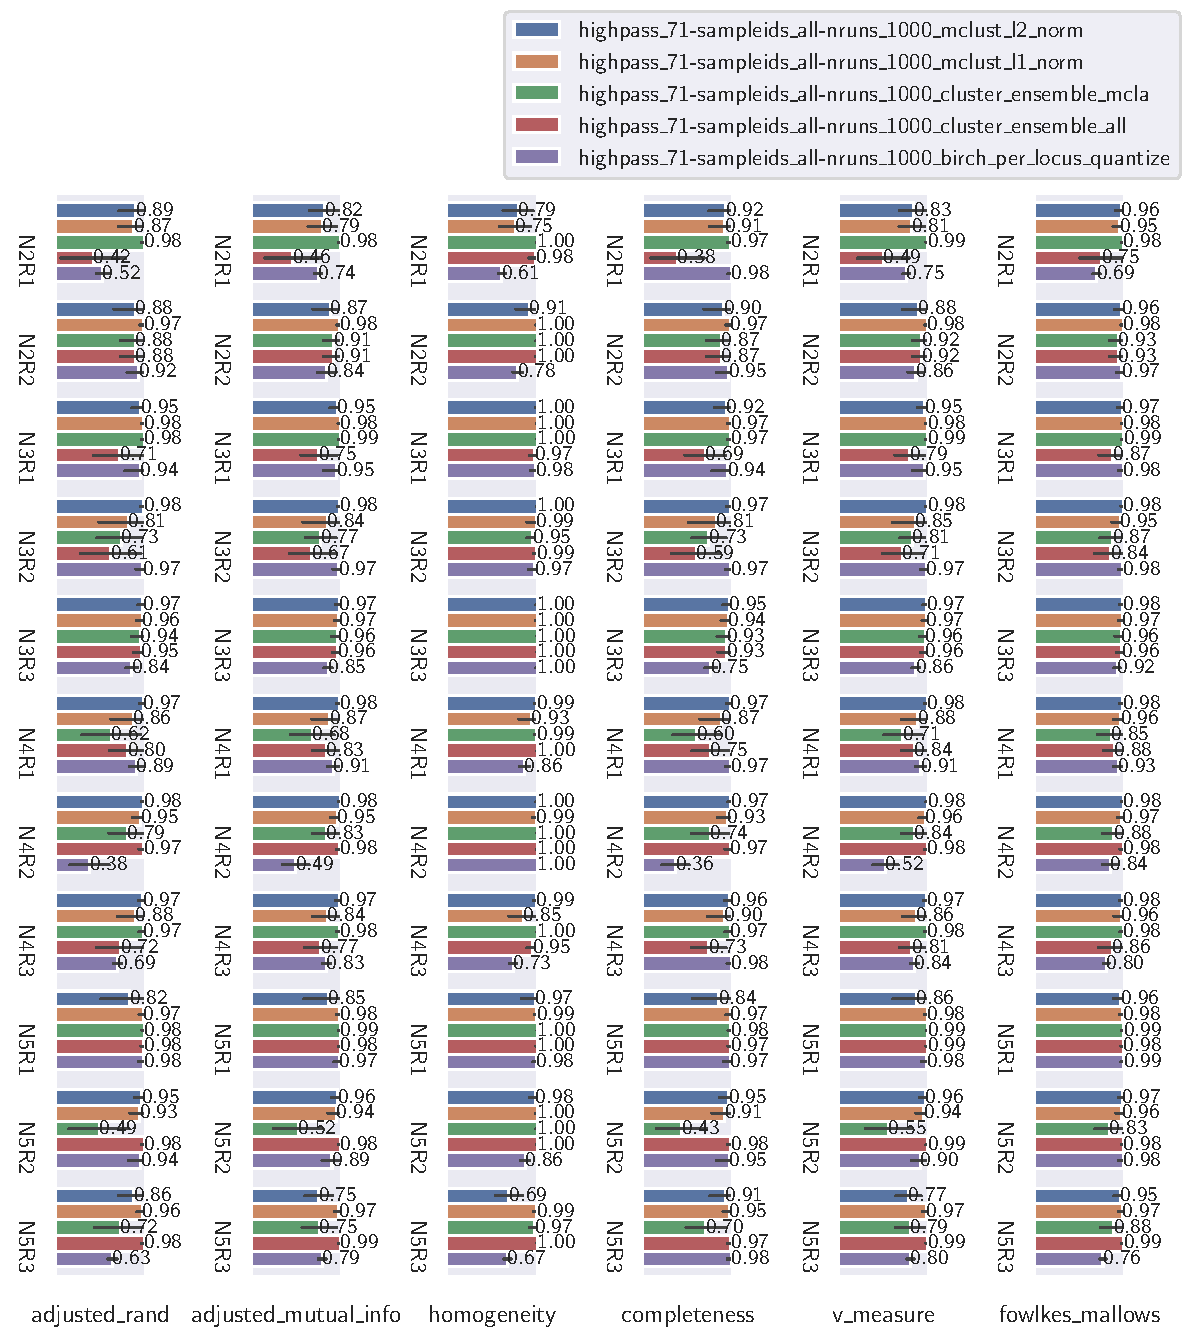
\includegraphics[width=\textwidth]{./figures/clust_comparison/highpass_71-sampleids_all-nruns_1000_top_5_clusterers_including_ensembles_by_metrics.pdf}
\caption{Top 5 clusterers, including ensembles, clustering performance metrics using 1000 trials sampled from all EPGs with high-pass filtering}
\label{fig:highpass_71-sampleids_all-nruns_1000_top_5_clusterers_including_ensembles_by_metrics}
\end{figure}

\begin{table}[H]
\centering
\maxsizebox{\textwidth}{0.65\textwidth}{
\begin{tabular}{lrr}
\toprule
{} &   mean &    std \\
clusterer                                          &        &        \\
\midrule
mclust\_l1\_norm                                     & 55.81\% & 16.52\% \\
mclust\_l2\_norm                                     & 55.11\% & 21.59\% \\
affinity\_per\_locus\_quantize                        & 43.65\% & 33.43\% \\
hdbscan\_cosine\_epsilon\_0.0\_eom\_per\_locus\_norm      & 43.43\% & 34.65\% \\
hdbscan\_euclidean\_epsilon\_0.0\_eom\_per\_locus\_norm   & 43.29\% & 34.62\% \\
hdbscan\_euclidean\_epsilon\_0.5\_eom\_per\_locus\_norm   & 43.29\% & 34.62\% \\
hdbscan\_euclidean\_epsilon\_1.0\_eom\_per\_locus\_norm   & 43.29\% & 34.62\% \\
affinity\_l2\_norm                                   & 42.88\% & 33.43\% \\
affinity\_per\_locus\_norm                            & 42.69\% & 33.26\% \\
hdbscan\_euclidean\_epsilon\_0.0\_eom\_per\_locus\_qua... & 42.66\% & 34.18\% \\
hdbscan\_euclidean\_epsilon\_0.0\_eom\_l2\_norm          & 42.08\% & 33.79\% \\
hdbscan\_euclidean\_epsilon\_0.5\_eom\_l2\_norm          & 42.08\% & 33.79\% \\
hdbscan\_cosine\_epsilon\_0.0\_eom                     & 41.60\% & 33.41\% \\
hdbscan\_euclidean\_epsilon\_0.5\_leaf\_l2\_norm         & 40.84\% & 32.82\% \\
cluster\_ensemble\_all                               & 39.63\% & 26.34\% \\
cluster\_ensemble\_mcla                              & 39.59\% & 26.27\% \\
affinity\_l1\_norm                                   & 38.79\% & 30.17\% \\
hdbscan\_euclidean\_epsilon\_0.0\_eom\_l1\_norm          & 32.90\% & 27.37\% \\
hdbscan\_cosine\_epsilon\_0.0\_eom\_per\_locus\_quantize  & 31.86\% & 25.94\% \\
hdbscan\_cosine\_epsilon\_0.5\_eom\_per\_locus\_norm      & 29.40\% & 27.16\% \\
hdbscan\_cosine\_epsilon\_0.5\_leaf\_per\_locus\_norm     & 29.40\% & 27.16\% \\
birch\_l2\_norm                                      & 25.36\% & 29.54\% \\
birch\_per\_locus\_norm                               & 23.08\% & 38.11\% \\
birch\_per\_locus\_quantize                           & 23.01\% & 38.01\% \\
optics\_per\_locus\_quantize                          & 18.10\% & 16.29\% \\
\bottomrule
\end{tabular}


}
\caption{Top 25 clusterers by arithmetic mean of percentages of perfect clustering, using admixtures sampled from all EPG data with highpass filter}
\label{table:top_25_clusterers_by_binomial_confidence_highpass_71-sampleids_all-nruns_1000}
\end{table}

\begin{table}[H]
\centering
\maxsizebox{\textwidth}{0.65\textwidth}{
\begin{tabular}{llrrrrrrrrrr}
\toprule
     & {} & \multicolumn{5}{l}{homogeneity} & \multicolumn{5}{l}{completeness} \\
     & clusterer &           1 &      2 &      3 &      4 &      5 &            1 &      2 &      3 &      4 &      5 \\
\midrule
N2R1 & ci\_upp &      23.94\% & 27.16\% & 97.39\% & 98.62\% &  4.02\% &       77.87\% & 83.97\% & 82.93\% & 86.33\% & 32.09\% \\
     & success &      21.30\% & 24.40\% & 96.40\% & 97.90\% &  2.80\% &       75.30\% & 81.70\% & 80.60\% & 84.20\% & 29.20\% \\
     & ci\_low &      18.87\% & 21.84\% & 95.06\% & 96.81\% &  1.94\% &       72.53\% & 79.18\% & 78.03\% & 81.81\% & 26.47\% \\
N2R2 & ci\_upp &      94.06\% & 64.27\% & 89.31\% & 98.78\% &  0.38\% &       65.06\% & 83.31\% &  9.85\% & 79.02\% & 31.07\% \\
     & success &      92.60\% & 61.30\% & 87.40\% & 98.10\% &  0.00\% &       62.10\% & 81.00\% &  8.00\% & 76.50\% & 28.20\% \\
     & ci\_low &      90.81\% & 58.24\% & 85.20\% & 97.05\% &  0.00\% &       59.05\% & 78.45\% &  6.47\% & 73.77\% & 25.50\% \\
N3R1 & ci\_upp &      90.88\% & 99.01\% & 94.96\% & 98.46\% & 50.60\% &       59.05\% & 76.24\% & 65.64\% & 72.57\% & 70.43\% \\
     & success &      89.10\% & 98.40\% & 93.60\% & 97.70\% & 47.50\% &       56.00\% & 73.60\% & 62.70\% & 69.80\% & 67.60\% \\
     & ci\_low &      87.02\% & 97.42\% & 91.91\% & 96.57\% & 44.42\% &       52.91\% & 70.78\% & 59.66\% & 66.88\% & 64.64\% \\
N3R2 & ci\_upp &      98.94\% & 94.87\% & 94.78\% &  0.38\% & 98.94\% &       75.85\% & 68.09\% &  6.08\% & 32.20\% & 65.55\% \\
     & success &      98.30\% & 93.50\% & 93.40\% &  0.00\% & 98.30\% &       73.20\% & 65.20\% &  4.60\% & 29.30\% & 62.60\% \\
     & ci\_low &      97.29\% & 91.80\% & 91.69\% &  0.00\% & 97.29\% &       70.37\% & 62.19\% &  3.47\% & 26.56\% & 59.56\% \\
N3R3 & ci\_upp &      96.71\% & 97.05\% & 96.27\% &  5.06\% &  0.38\% &       66.33\% & 71.21\% & 72.76\% & 29.01\% & 35.97\% \\
     & success &      95.60\% & 96.00\% & 95.10\% &  3.70\% &  0.00\% &       63.40\% & 68.40\% & 70.00\% & 26.20\% & 33.00\% \\
     & ci\_low &      94.14\% & 94.60\% & 93.58\% &  2.70\% &  0.00\% &       60.37\% & 65.45\% & 67.09\% & 23.57\% & 30.16\% \\
N4R1 & ci\_upp &      74.60\% & 82.74\% & 96.96\% & 98.14\% & 98.62\% &       78.54\% & 62.11\% &  4.25\% & 69.65\% & 72.37\% \\
     & success &      71.90\% & 80.40\% & 95.90\% & 97.30\% & 97.90\% &       76.00\% & 59.10\% &  3.00\% & 66.80\% & 69.60\% \\
     & ci\_low &      69.03\% & 77.83\% & 94.49\% & 96.10\% & 96.81\% &       73.26\% & 56.02\% &  2.11\% & 63.82\% & 66.68\% \\
N4R2 & ci\_upp &      93.53\% & 89.31\% & 98.78\% &  0.38\% &  0.38\% &       74.89\% & 60.63\% & 73.44\% & 26.12\% & 33.22\% \\
     & success &      92.00\% & 87.40\% & 98.10\% &  0.00\% &  0.00\% &       72.20\% & 57.60\% & 70.70\% & 23.40\% & 30.30\% \\
     & ci\_low &      90.15\% & 85.20\% & 97.05\% &  0.00\% &  0.00\% &       69.34\% & 54.51\% & 67.80\% & 20.88\% & 27.53\% \\
N4R3 & ci\_upp &      45.49\% & 87.17\% & 98.70\% &  0.38\% & 97.56\% &       80.65\% & 69.94\% & 66.62\% & 32.40\% & 76.72\% \\
     & success &      42.40\% & 85.10\% & 98.00\% &  0.00\% & 96.60\% &       78.20\% & 67.10\% & 63.70\% & 29.50\% & 74.10\% \\
     & ci\_low &      39.37\% & 82.76\% & 96.93\% &  0.00\% & 95.29\% &       75.54\% & 64.13\% & 60.67\% & 26.76\% & 71.30\% \\
N5R1 & ci\_upp &      85.39\% & 97.89\% & 97.81\% & 97.89\% & 99.16\% &       61.12\% & 79.69\% & 59.15\% & 65.55\% & 78.93\% \\
     & success &      83.20\% & 97.00\% & 96.90\% & 97.00\% & 98.60\% &       58.10\% & 77.20\% & 56.10\% & 62.60\% & 76.40\% \\
     & ci\_low &      80.76\% & 95.75\% & 95.63\% & 95.75\% & 97.66\% &       55.02\% & 74.50\% & 53.01\% & 59.56\% & 73.67\% \\
N5R2 & ci\_upp &      98.62\% & 89.31\% & 99.59\% & 51.90\% & 98.38\% &       71.89\% & 79.41\% & 79.41\% & 71.11\% & 69.65\% \\
     & success &      97.90\% & 87.40\% & 99.20\% & 48.80\% & 97.60\% &       69.10\% & 76.90\% & 76.90\% & 68.30\% & 66.80\% \\
     & ci\_low &      96.81\% & 85.20\% & 98.43\% & 45.71\% & 96.45\% &       66.17\% & 74.19\% & 74.19\% & 65.35\% & 63.82\% \\
N5R3 & ci\_upp &      88.94\% & 11.04\% & 91.98\% & 96.88\% & 99.01\% &       65.84\% & 79.69\% &  8.64\% & 76.43\% & 86.14\% \\
     & success &      87.00\% &  9.10\% & 90.30\% & 95.80\% & 98.40\% &       62.90\% & 77.20\% &  6.90\% & 73.80\% & 84.00\% \\
     & ci\_low &      84.77\% &  7.47\% & 88.31\% & 94.37\% & 97.42\% &       59.86\% & 74.50\% &  5.49\% & 70.99\% & 81.60\% \\
\bottomrule
\end{tabular}


}
\caption{Top 5 clusterers, including ensembles, clustering percentages of trials where no error occurs using 1000 trials sampled from all EPGs with high-pass filtering}
\label{table:highpass_71-sampleids_all-nruns_1000_top_5_clusterers_including_ensembles_by_binomial_confidence}
\end{table}

%--------------------------------------------------------------------------------------------------------------------------------------------
\chapter{Software Work}
\thispagestyle{myheadings}
\label{appendix:Software Work}

A large amount of work involved in this thesis is under the surface in the software.

\section{Software Setup}

\subsection{Code Repositories}

A copy of the software code for this thesis is in the following locations:

\begin{itemize}
  \item \url{https://github.com/dougjih/thesis-code-ms-cs-rutgers}: code for experiments presented in the thesis
  \item \url{https://github.com/dougjih/thesis-doc-ms-cs-rutgers}: code for the thesis document
  \item \url{https://github.com/dougjih/single-cell-cluster}: early experimental and exploratory code for various ideas
\end{itemize}

These repositories currently allow only private access at the direction of the LFTDI, which owns the input data for the experiments.

\subsection{Programming Environment}

The software code of this project is written in the Python programming language. Python 3.9.2 is used with a venv. Some supporting functions are implemented in makefile and shell scripts.

For mclust, R version 4.0.4 is used. Mclust version 5.4.7 is used. The Python package rpy2 is used to run R and mclust in a Python process \cite{noauthor_rpy2_nodate}.

For software development, Git and Visual Studio Code, GNU Make, and GNU Bash are used.

For reference management, Zotero is used.

For thesis production, Miktex and TeXworks are used.

\subsection{Python Packages}

The software code in this thesis imports the Python packages shown in Table \ref{table:Python Packages}. Transitive dependencies are not shown. Pip, a package-management system for Python, is used.

\begin{table}
\centering
\begin{tabular}{ll}
\toprule
         Package & Version \\
\midrule
ClusterEnsembles &   1.0.1 \\
         hdbscan &  0.8.28 \\
          joblib &   1.1.0 \\
      matplotlib &   3.5.1 \\
           numpy &  1.22.3 \\
          pandas &   1.4.1 \\
            rpy2 &   3.4.5 \\
    scikit-learn &   1.0.2 \\
         seaborn &  0.11.2 \\
     statsmodels &  0.13.2 \\
\bottomrule
\end{tabular}
\caption{Python packages used in the thesis software code}
\label{table:Python Packages}
\end{table}

\section{Hardware Setup}

The computational experiments in this thesis were done on a personal computer with the components shown in Table \ref{table:Computer Configuration}.

\begin{table}
\centering
\begin{tabular}{ll}
\toprule
                     Component &                                        Model \\
\midrule
                           CPU &                            AMD Ryzen 9 5900X \\
                           RAM &                              32 GB DDR4 3200 \\
                           GPU &                        AMD Radeon RX 5700 XT \\
       Operating System (Host) & Windows 11 (original release, latest update) \\
               Virtual Machine &                Windows Subsystem for Linux 2 \\
Operating System (Development) &                                  Debian 11.2 \\
\bottomrule
\end{tabular}
\caption{Computer Configuration}
\label{table:Computer Configuration}
\end{table}

\section{Known Issues}

\subsection{Parallelization}

Many of the various software libraries cannot or do not automatically parallelize their computational workloads. In particular, mclust is time-consuming and appears to saturate only two threads. Pandas also does not parallelize much of its work.

Where feasible, easy parallelization is done by using Joblib in Python and running multiple processes with GNU Make and in Bash scripts.

For a solution that is truly distributed and more flexible, Dask is promising.

\subsection{Memory Limitation}

Computer memory limitation is a problem for running computation work on the data sets in this project, especially when multiple workloads are run in parallel. Much of this is due to the simplistic implementation of the code that loads all the data into memory. A more sophisticated implementation that streams the data, or one that uses a backend with a ``lazy execution'' approach such as that Dask provides, can mitigate much of the problem.


\end{theappendices}